\chapter{$H \to ZZ \to 4\ell$ search \& Production/Decay Fractions}
\label{sec:4l_Experiment}
\chaptermark{$H \to ZZ \to 4\ell$ search \& Production/Decay Fractions}


In this section we discuss the search for a Higgs boson decaying to the 4 lepton final state at CMS. First, we will provide a general overview of the analysis. Next, we will discuss additional requirements that are made on the physics objects we have already introduced. Using this information we will present the event selection, simulation, and categorization for the search and a summary of the expected signal and background estimations. Next, we will introduce the kinematic distributions that are used to enhance our signal against the background processes. Specifically, the $m_{4\ell}$ mass shape, the \textit{Matrix Element Likelihood Approach} (MELA) kinematic discriminant, the $p_{T}^{4\ell}$, and the jet kinematic discriminant. Finally we will present the results of this search and first major characterization study: The production and decay fraction measurements. The studies presented in this section have been published in reference \cite{Chatrchyan:2013mxa}.

\section{General overview of $H \to ZZ \to 4l$}
\label{sec:General_H_ZZ_4l}

While some of this information was introduced earlier in order to discuss specific theoretical and phenomenological aspects of this work, here we will summarize the $H \to ZZ \to 4\ell$ search. This analysis searches for a scalar Higgs boson which would be the smoking gun that the Higgs Mechanism is responsible for electroweak symmetry breaking. This search covers the range of $m_{4\ell} \in \unit{110--1000}{\GeV}$ because the mass of the Higgs boson $\left(m_{H}\right)$ is a free parameter in the theoretical basis for the theory. General theoretical considerations suggest that $m_{H}$ should be less than $\approx \unit{1}{\TeV}$ \cite{PhysRevD.10.1145, PhysRevD.16.1519, PhysRevLett.30.1268, LlewellynSmith1973233}, while precision electroweak measurements imply that $m_{H} < \unit{152}{\GeV}$ \cite{ALEPH:2010aa}. Previously, direct searches for the Higgs boson have been made at the LEP collider setting the limit that $m_{H} > \unit{114.4}{\GeV}$ \cite{Barate:2003sz}, and the Tevatron collider, excluding $m_{H} \notin \unit{90--109}{\GeV}\cup\unit{149--182}{\GeV}$ \cite{Aaltonen:2013xpo, Aaltonen:2012qt}.

In this thesis, the analysis of the $H \to ZZ \to 4\ell$ channel is presented using the entire dataset collected by the CMS experiment during the 2011-2012 LHC running period. The data correspond to an integrated luminosity of $\unit{5.1}{\invfemtobarn}$ of proton-proton collisions at a center of mass energy of $\sqrt{s} = \unit{7}{\TeV}$, and $\unit{19.7}{\invfemtobarn}$ at $\sqrt{s} = \unit{8}{\TeV}$. The search looks for a signal consisting of two pairs of same-flavor, opposite-charge, well-identified and isolated leptons compatible with a $ZZ$-system, appearing as a narrow resonance on top of a smooth background in the four-lepton invariant mass distribution.

\section{Object Selection}
\label{sec:Obj_select}

Given the very low branching fraction of the $H \to ZZ \to 4\ell$ decay, it is important to maintain a very high lepton selection efficiency in a wide range of momenta, to maximize the sensitivity for a Higgs boson in the full range $m_{4\ell} \in \unit{110--1000}{\GeV}$. Additionally, because the signal sensitivity depends on the $4\ell$ mass resolution it is crucial to calibrate the individual lepton momentum scale and resolution to a level such that the systematic uncertainties are small. A summary of the lepton identification, scale, and resolution is presented in section \ref{sec:TriggerANDreconstruction}. Additional object selections including lepton isolation and vertex compatibility are presented here.

Lepton isolation is used to discriminate leptons originating from high-$p_{T}$ boson decay, as in the case of the signal, from those arising from hadronic processes, which are typically immersed in a jet of other hadrons. The isolation of individual leptons, measured relative to their
transverse momentum $p_{T}^{\ell}$, is defined by:

\begin{equation}
\label{eqn:pfiso}
R_\text{Iso}^{\ell} \equiv \Big( \sum p_{T}^\text{charged} +
                                 \max\big[ 0, \sum p_{T}^\text{neutral}
                                 +
                                  \sum p_{T}^{\gamma}
                                 - p_{T}^\mathrm{PU}(\ell) \big] \Big)
                                 / p_{T}^{\ell},
\end{equation}

where the sums are over the charged, neutral, and photon particle candidates in a cone $\Delta R = \sqrt{\left(\Delta\eta\right)^{2} + \left(\Delta\phi\right)^{2}} < 0.4$ around the lepton direction at the interaction vertex (where $\Delta\eta\text{ \& }\Delta\phi$ quantify the angular distance between the candidate from the lepton). In equation \eqref{eqn:pfiso}, the sums are computed for particles that originate from the primary vertex of the event (defined as the vertex with the the highest  $\sum p_{T}^{2}$ of associated tracks). In this expression, the contribution from pileup $\left(p_{T}^{PU}\left(\ell\right)\right)$ is explicitly subtracted. This pileup contribution is computed separately for electrons and muons and outlined in \cite{Chatrchyan:2013mxa}. In this isolation calculation, photons that qualify for FSR reconstruction are omitted from the $p_{T}^{\gamma}$ sum. FSR is outlined in the muon reconstruction section \ref{sec:Muons}.

In order to suppress leptons originating from in-flight decays of hadrons and muons from cosmic rays, all leptons are required to come from the same primary vertex. This is achieved by requiring that the significance of the interaction parameter in three dimensions is $\text{SIP}_{\text{3D}} < 4$, where $\text{SIP}_{\text{3D}} \equiv \text{IP}_{\text{3D}}/\sigma_{\text{IP}_{\text{3D}}}$ is the ratio of the impact parameter of the lepton track in three dimensions, with respect to the chosen primary vertex position, and its uncertainty.

The combined efficiency for the reconstruction, identification, and isolation (and conversion rejection for electrons) of prompt electrons or muons is measured in data using a �tag and probe� method based on an inclusive sample of Z-boson events, separately for 7 and $\unit{8}{\TeV}$ data. The efficiency is measured by fitting the Z line shape plus a background model to the dilepton mass distributions where the probe lepton passes or fails the selection criteria. This efficiency is calculated in both simulation and data and used to correct the simulation accordingly. These efficiencies are shown in figure \ref{fig:lepeff} for both electrons and muons.

\begin{figure}
  \begin{center}
      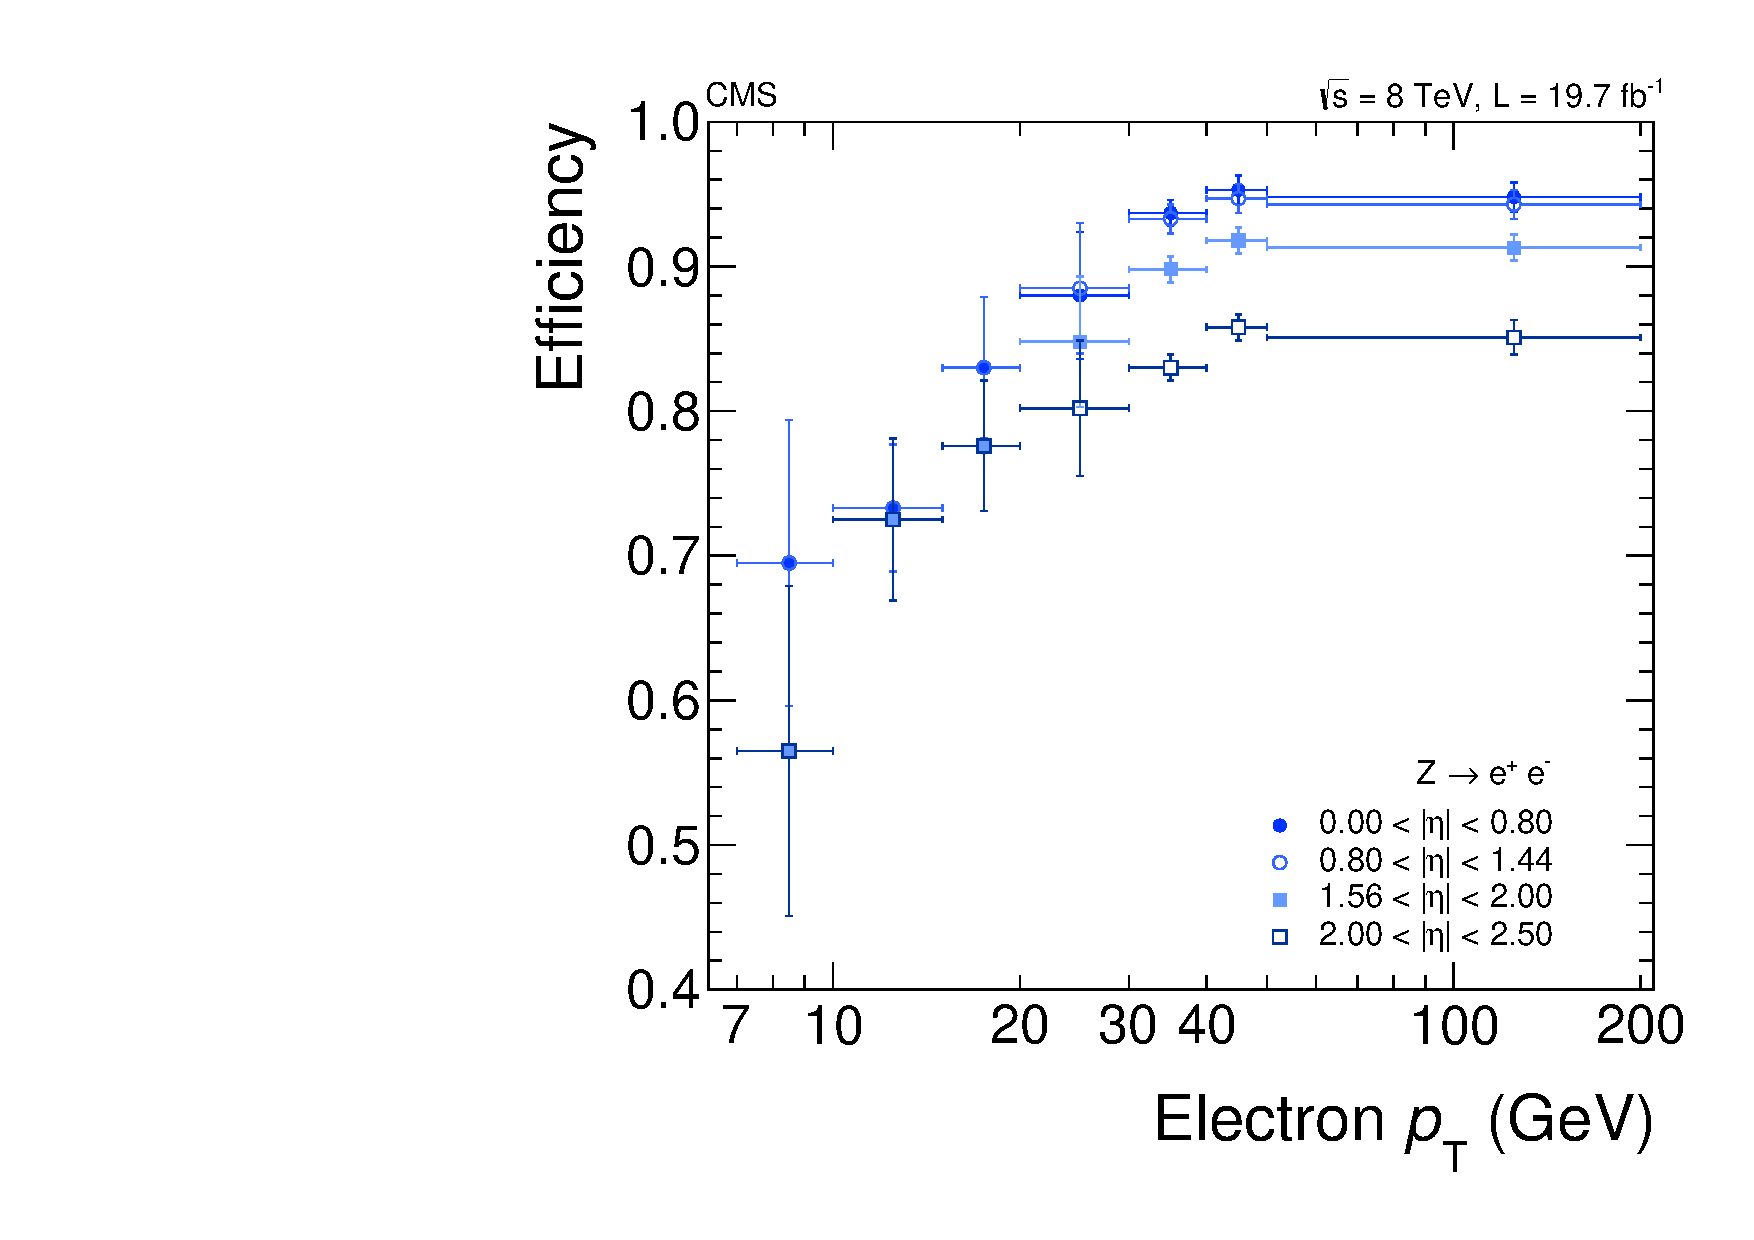
\includegraphics[width=0.45\linewidth]{{HZZ4l_search/electron_efficiency}.pdf}
      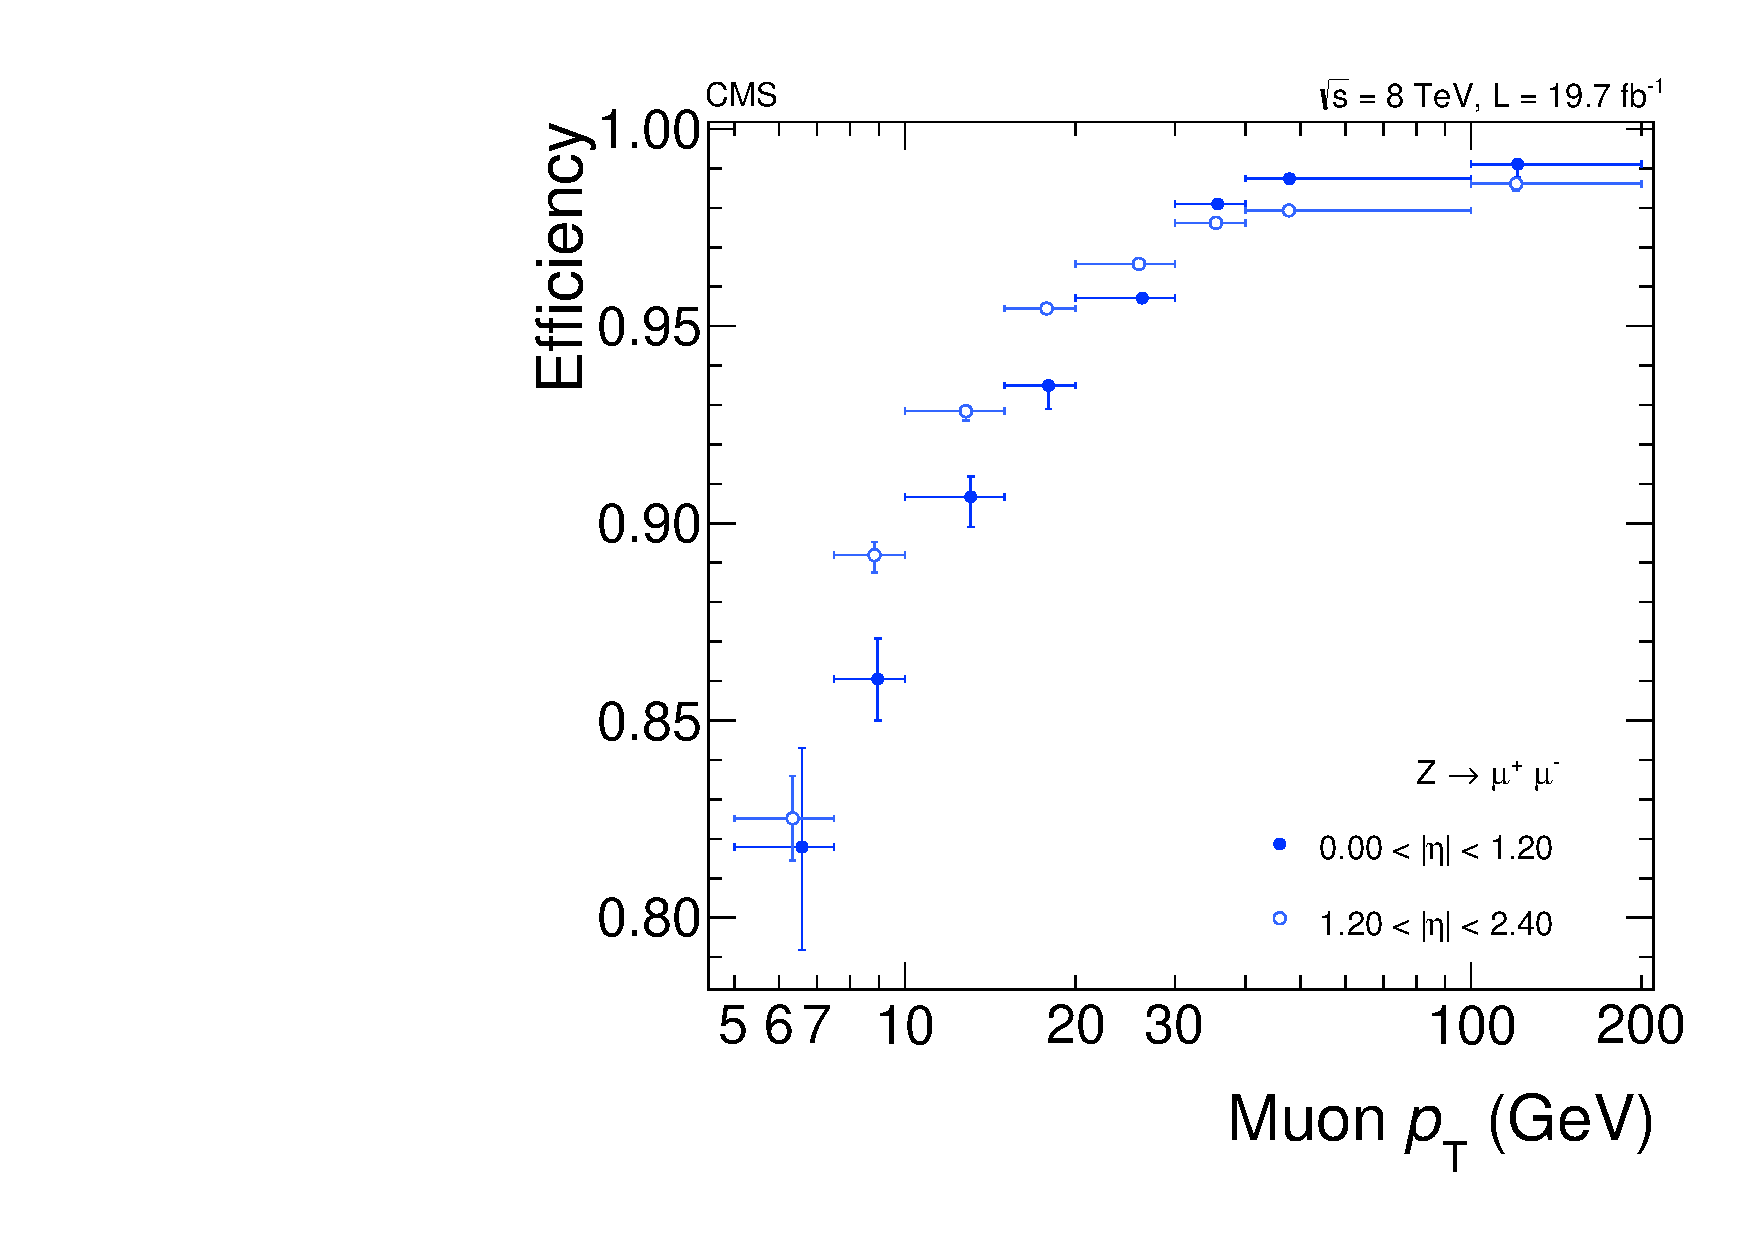
\includegraphics[width=0.45\linewidth]{{HZZ4l_search/muon_efficiency}.pdf}
    \caption[Efficiency, as a function of the lepton $p_{T}^\ell$, for
      reconstructing and selecting (left) electrons and
      (right) muons, measured with a $Z \to \ell\ell$ data sample
      by using a tag-and-probe method.]{Efficiency, as a function of the lepton $p_{T}^\ell$, for
      reconstructing and selecting (left) electrons and
      (right) muons, measured with a $Z \to \ell\ell$ data sample
      by using a tag-and-probe method \cite{Chatrchyan:2013mxa}.}
\label{fig:lepeff}
\end{center}
\end{figure}

In the analysis the presence of jets is used as an indication of vector-boson fusion (VBF) or associated production with a weak boson, $VH$, with $V$ = $W$ or $Z$, where the $V$ decays hadronically. Jets are reconstructed using the anti-$k_{T}$ clustering algorithm with distance parameter $D=0.5$, as discussed in section \ref{sec:Jets}. Jets are only
considered if they have $p_{T}^\text{jet}>\unit{30}{\GeV}$, $\abs{\eta^\text{jet}}<4.7$, originate from the primary vertex, and are required to be separated from the lepton candidates and from identified FSR photons by $\Delta R > 0.5$. Jet energy corrections are applied as a function of the jet $p_{T}^\text{jet}$ and $\eta^\text{jet}$~\cite{Chatrchyan:2011ds}. An offset correction is applied to subtract the energy contribution not associated with the high-$p_{T}$ scattering, such as electronic noise and pileup, based on the jet-area method~\cite{Chatrchyan:2011ds,Cacciari:2007fd,Cacciari:2008gn}.

\section{Event Selection, Simulation, \& Categorization}
\label{sec:Selection_Simulation_Categorizaiton}

\subsection{Simulated Data Samples}

The Monte Carlo (MC) simulated data samples, generated with state-of-the-art theoretical calculations for both the SM Higgs boson signal and relevant background processes, are used to optimize the event selection and to evaluate the acceptance and systematic uncertainties. For the gluon-gluon fusion and vector-boson fusion Higgs boson signal the simulated events are generated with \textsc{powheg} \cite{Nason:2009ai, Bagnaschi:2011tu, Frixione:2007vw} at Next-to-leading-order (NLO) QCD accuracy. The Higgs boson decay is modeled with \textsc{JHUGen} 3.1.8 \cite{Gao:2010qx, Bolognesi:2012mm, Anderson:2013afp} to include proper treatment of the interference effects associated with permutations of identical leptons in the four-electron and four-muon final states. Samples of WH, ZH, and $t\bar{t}H$ events are generated with \textsc{PYTHIA} 6.4.24 \cite{Sjostrand:2006za}. Higgs boson signal events for all production mechanisms are reweighted to include contributions from gluon fusion up to next-to-next-to-leading-order (NNLO) and next-to-next-to-leading logarithm (NNLL) \cite{Dawson1991283, Djouadi1991440, Actis:2008ug, Catani:2003zt, Ravindran:2003um, Anastasiou:2002yz, Harlander:2002wh, Spira:1995rr, Dittmaier:2011ti, Baglio:2010ae, Anastasiou:2008tj, deFlorian:2012mx}, and from the vector-boson fusion contribution computed at NNLO \cite{Dittmaier:2011ti, Ciccolini:2007jr, Ciccolini:2007ec, Figy:2003nv, Arnold:2008rz, Bolzoni:2010xr}.

The two dominant irreducible background contributions for this analysis are the SM $q\bar{q} \to ZZ$ and $gg \to ZZ$ events. The $q\bar{q} \to ZZ$ background is simulated at NLO using the \textsc{powheg} \cite{Melia:2011tj} program while the $gg \to ZZ$ contribution is simulated at LO using \textsc{GG2ZZ} \cite{Binoth:2008pr}. The yields for these SM congribitons are calculated with \textsc{MCFM} \cite{Campbell:2011bn, Campbell:1999ah, Campbell:2010ff}. The reducible backgrounds including, $Zb\bar{b}$, $Zc\bar{c}$, $Z\gamma + \text{jets}$, $WW + \text{jets}$, $WZ + \text{jets}$, etc. (referred to as $Z + \text{jets}$) are simulated with \textsc{MADGRAPH} \cite{Alwall:2007st} and used to cross check the data driven methods outlined in the next section (The $t\bar{t}$ contribution to this background is simulated at NLO with \textsc{POWHEG}).

To model the constituents (quarks \& gluons) of the colliding protons correctly, parton distributions functions are used (\textsc{CTEQ6L} \cite{Lai:2010nw} for LO generators, \textsc{CT10} \cite{Lai:2010vv} for NLO and higher-order generators). To model the underlying event, jet fragmentation, and showering all events are processed with \textsc{PYTHIA} 6.4.24 \cite{Sjostrand:2006za}. The CMS detector is simulated with great detail using a simulation based on \textsc{GEANT4} \cite{Agostinelli2003250, Allison:2006ve}.

\subsection{Selection \& Categorization}

The event selection is designed to give a set of signal candidates in the $H \to ZZ \to 4\ell$ final state in three mutually exclusive subchannels: $4e$, $4\mu$, and $2e2\mu$. Four well-identified and isolated leptons are required to originate from the primary vertex to suppress the $Z + \text{jets}$ and $t\bar{t}$ backgrounds.

Z candidates are formed with a pair of leptons of the same flavor and opposite charge $\left(\ell^{+}\ell^{-}\right)$. When forming the Z-boson candidates, only FSR photons that make the lepton-pair mass closer to the nominal Z-boson mass are incorporated. If the $m_{\ell\ell\gamma}>\unit{100}{\GeV}$, the photon is not considered, to minimize the fraction of misidentification. 

Among all the possible opposite-charge lepton paris in the event, the one with an invariant mass closest to the nominal Z-boson mass is denoted $Z_{1}$ and retained if $40 < m_{Z_{1}} < \unit{120}{\GeV}$. Then, all remaining leptons are considered and a second same flavor opposite-charge pair $\ell^{+}\ell^{-}$ becomes $Z_{2}$ when the pair has the highest scalar sum of $p_{T}^{\ell\ell}$ in the event and $12 < m_{Z_2} <\unit{120}{\GeV}$. This selection procedure results in one or more of the Z-bosons to be off shell for $m_{H} < \unit{180}{\GeV}$. 

Among the four selected leptons forming the $Z_1$ and the $Z_2$,
at least one lepton is required to have $p_{T}^\ell > \unit{20}{\GeV}$, and
another one is required to have $p_{T}^\ell > \unit{10}{\GeV}$.  These
$p_{T}^\ell$ thresholds ensure that the selected events have leptons on
the efficiency plateau of the trigger.  To further remove events with
leptons originating from hadron decays produced by jet fragmentation
or from the decay of low-mass hadron resonances, it is required that
any opposite-charge pair of leptons chosen among the four selected
leptons (irrespective of flavor) satisfy $m_{\ell^+\ell^-} > \unit{4}{\GeV}$.
The phase space for the search of the SM Higgs boson is defined by
restricting the measured mass range to $m_{4\ell} > \unit{100}{\GeV}$.

The efficiency versus $m_{H}$ is shown in Fig.~\ref{fig:effMH} for the gluon fusion Higgs boson production mode, and it is very similar for other production modes. The efficiency within the geometrical acceptance is $\approx$30\%~(58\%),
43\%~(71\%), and 62\%~(87\%) for the $4e, 2e2\mu, \text{ and } 4\mu$ channels, respectively, for $m_H = \unit{126(200)}{\GeV}$.

\begin{figure}
  \begin{center}
    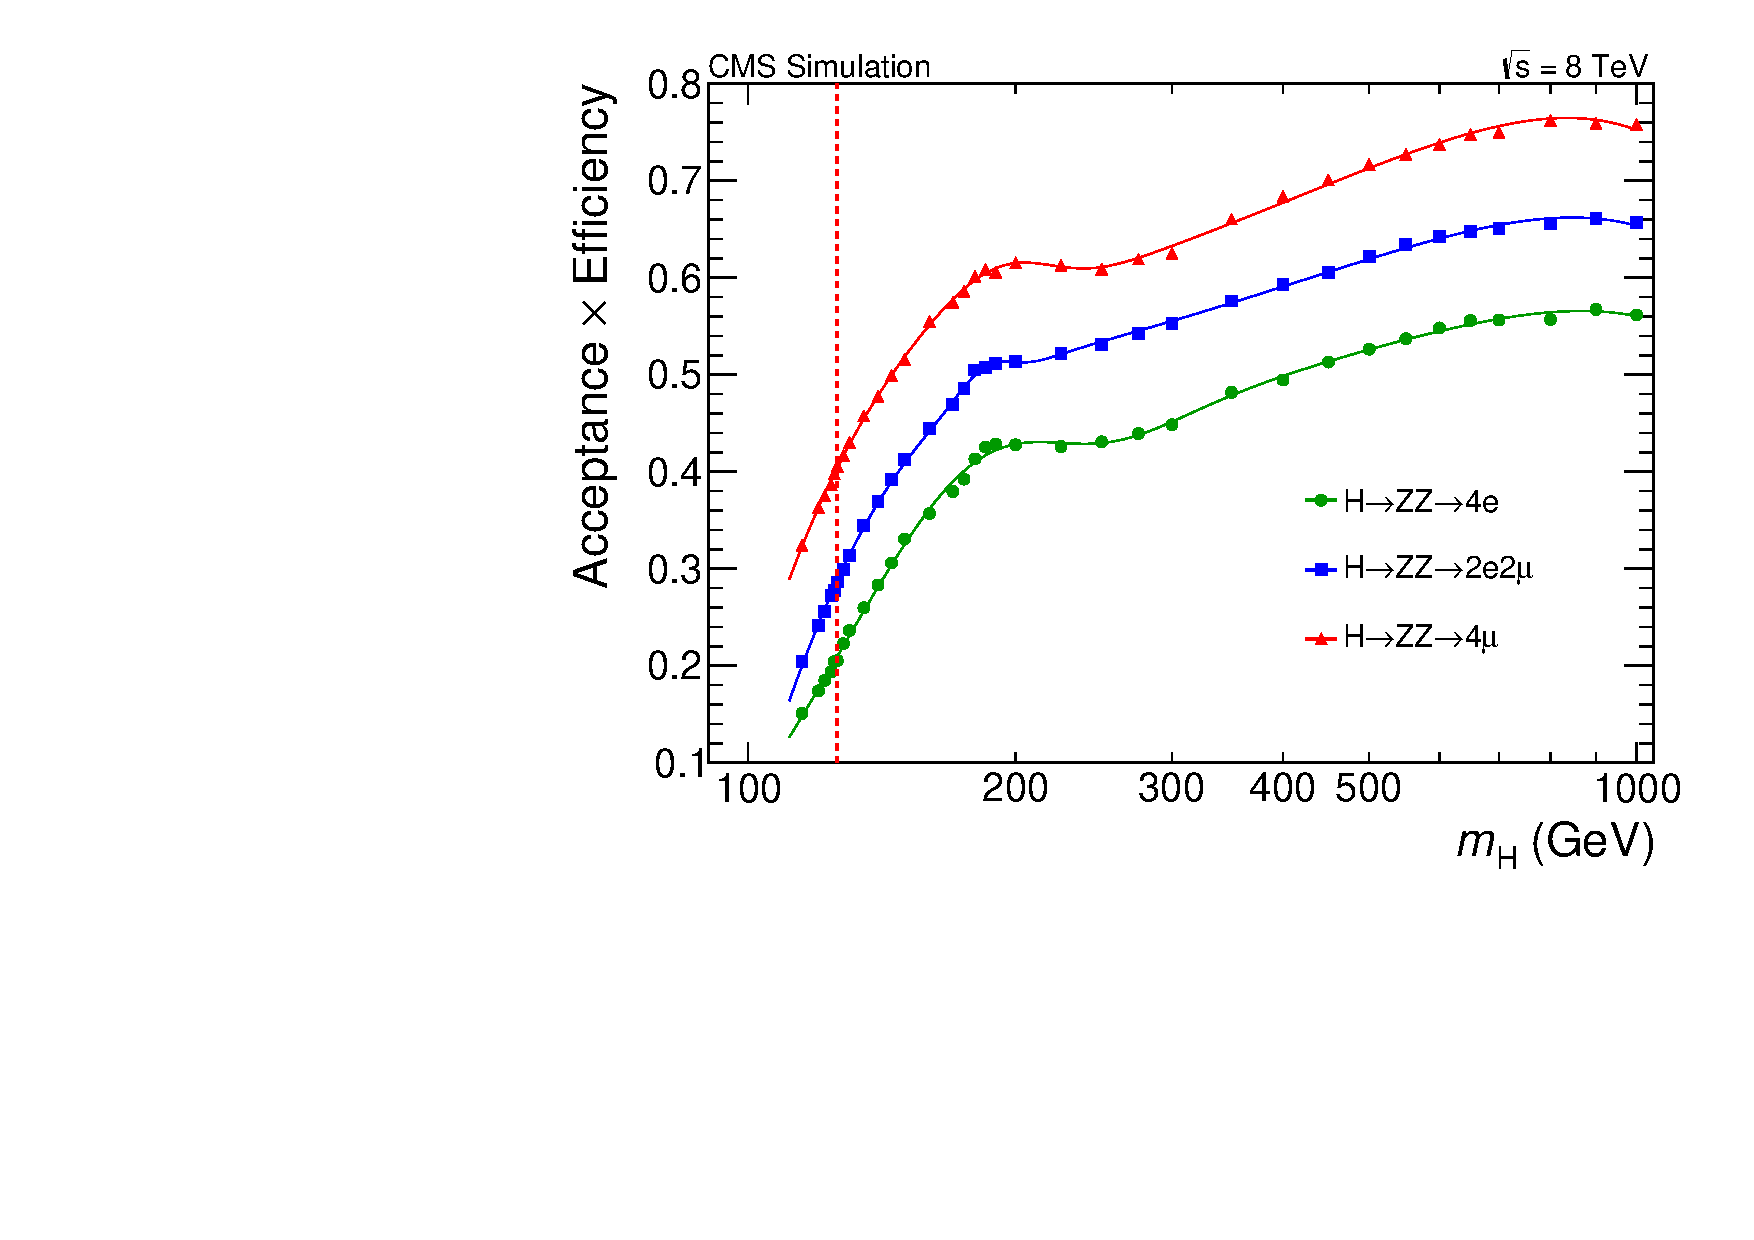
\includegraphics[width=0.65\textwidth]{HZZ4l_search/Efficiency_ggH_8TeV.pdf}
    \caption[Geometrical acceptance times selection efficiency for the SM Higgs boson signal as a function of $m_H$ in the three final states for gluon fusion production. Points represent efficiency estimated from full CMS simulation; lines represent a smooth polynomial curve interpolating the points, used in the analysis. The vertical dashed line represents $m_H = \unit{126}{\GeV}$.]{Geometrical acceptance times selection efficiency for the SM Higgs boson signal as a function of $m_H$ in the three final states for gluon fusion production. Points represent efficiency estimated from full CMS simulation; lines represent a smooth polynomial curve interpolating the points, used in the analysis. The vertical dashed line represents $m_H = \unit{126}{\GeV}$ \cite{Chatrchyan:2013mxa}.}
      \label{fig:effMH}
\end{center}
\end{figure}

In order to improve the sensitivity to the Higgs boson production mechanisms, the event sample is split into two categories based on the jet multiplicity. These categories are defined as the 0/1-jet category, containing events with fewer than two jets, and the dijet category, containing events with at least two jets.

\subsection{Background estimation}
\label{sec:BkgEstimation}

The dominant background contribution in the $H \to ZZ \to 4\ell$ search is irreducible and is due to direct ZZ production via $q\bar{q}$ annihilation and gluon fusion. The remaining subleading contributions arise from reducible multilepton sources, $Z + \text{jets}$, $t\bar{t}$, and $WZ + \text{jets}$.

The expected yield and shape of the $q\bar{q} \to ZZ$ and $gg \to ZZ$ background is evaluated using the simulated events discussed above. The $gg \to ZZ$ contribution with respect to the $q\bar{q} \to ZZ$ varies from about $2\%$ at $m_{4\ell} = \unit{126}{\GeV}$ to $6\%$ at $m_{4\ell} = \unit{1}{\TeV}$. These two background processes make up a huge fraction of the total background in this analysis. In the region $100 < m_{4\ell} < \unit{1000}{\GeV}$ is approximately $91\%, 94\%,\text{ and } 97\%$ in the $4e, 2e2\mu, \text{ and } 4\mu$ decay channels, respectively. Within the smaller range around the observed peak $\left(121.5 < m_{4\ell} < \unit{130.5}{\GeV}\right)$ these irreducible backgrounds contribute $58\%, 71\%,\text{ and } 86\%$, respectively.

The Reducible background from $Z + \text{jets}$ is estimated using two independent methods. These methods use dedicated control regions in data where there is a dilepton pair satisfying all the requirements of a $Z_{1}$ candidate and two additional leptons satisfying certain relaxed identification requirements. In both methods, the extrapolation from the control region to the signal regions is performed using the lepton misidentification probability, $f\left(\ell,p_{T}^{\ell},\abs{\eta^{\ell}}\right)$, which is defined as the fraction of non-signal leptons identified in the analysis selection criteria evaluated on a sample of enriched non-genuine electrons and muons.

The first method uses two control regions that have a $Z_{1}$ candidate and two additional leptons with the same flavor and opposite charge. There are two categories of events that satisfy the criteria, 2P2F (composed of two leptons that pass selection and two that fail the selection criteria) and 3P1F (composed of three leptons that pass selection and one that fails). For each event $i$ that falls into the 2P2F or 3P1F category a weight factor of $\frac{f_{3}^{i}}{1- f_{3}^{i}}\frac{f_{4}^{i}}{1- f_{4}^{i}}$ or $\frac{f_{a}^{i}}{1- f_{a}^{i}}$ for the third and/or fourth leptons. The 3P1F region will also have a contribution from the reducible background and so the contribution is reduced by a factor of $\left(1 - \frac{n_{3P1F}^{ZZ}}{N_{3P1F}}\right)$ where $n_{3P1F}^{ZZ}$ is the estimation of irreducible ZZ events and $N_{3P1F}$ is the total number of events in the 3P1F region. The contribution of the 2P2F to the 3P1F is also accounted for and in the end the reducible background estimation in the signal region, $N_{SR}^{reducible}$, is given by equation \eqref{eq:PredictionSR},

\begin{equation}
  \label{eq:PredictionSR}
  N^\text{reducible}_\mathrm{SR} =
  \left( 1 - \frac{n^{ZZ}_\mathrm{3P1F}}{N_\mathrm{3P1F}} \right)
  \sum_j^{N_\mathrm{3P1F}} \frac{f^j_a}{1-f^j_a}-
  \sum_i^{N_\mathrm{2P2F}} \frac{f^i_3}{1-f^i_3} \frac{f^i_4}{1-f^i_4}.
\end{equation}

The second method uses a control region that has a $Z_{1}$ candidate and two additional leptons with the same flavor and the same charge. This method exploits the linear dependence of the $f\left(\ell,p_{T}^{\ell},\abs{\eta^{\ell}}\right)$ probability on the fraction of loose electrons with tracks have one missing hit in the pixel detector $r_{\text{miss}}\left(p_{T}^{e},\abs{\eta^{e}}\right)$, which is indicative of a possible FSR photon conversion. This $r_{\text{miss}}$ fraction is estimated using samples with different FSR contributions and the $f\left(\ell,p_{T}^{\ell},\abs{\eta^{\ell}}\right)$ is corrected to ${\tilde f}\left(\ell,p_{T}^{\ell},\abs{\eta^{\ell}}\right)$ using the corresponding $r_{\text{miss}}$ fraction.
The expected number of reducible background events in the signal region is given by equation \eqref{eq:PredictionSR_2}, where $N_{2P2F_{SS}}$ is the number of observed events in the same-sign 2P2F region. The ratio $r_\mathrm{OS/SS}$ between the number of events in the 2P2F opposite-sign and same-sign control regions is obtained from simulation.

\begin{equation}
\label{eq:PredictionSR_2}
  N^\text{reducible}_\mathrm{SR} =
  r_\mathrm{OS/SS} \, \cdot \,
  \sum_i^{N_\mathrm{2P2L_{SS}}}  \tilde f^i_3  \cdot \tilde f^i_4
\end{equation}

Both of these two reducible background estimations agree well within their statistical uncertainties. Such good agreement allows the analysis to combine the two estimations of the background together, assigning a systematic unvartainty of $20\%, 25\%, \text{ and } 40\%$ for the $4e, 2e2\mu, \text{ and } 4\mu$ decay channels, respectively. Validations of these two methods are shown in figure \ref{fig:zx}.

 \begin{figure}
 \begin{center}
   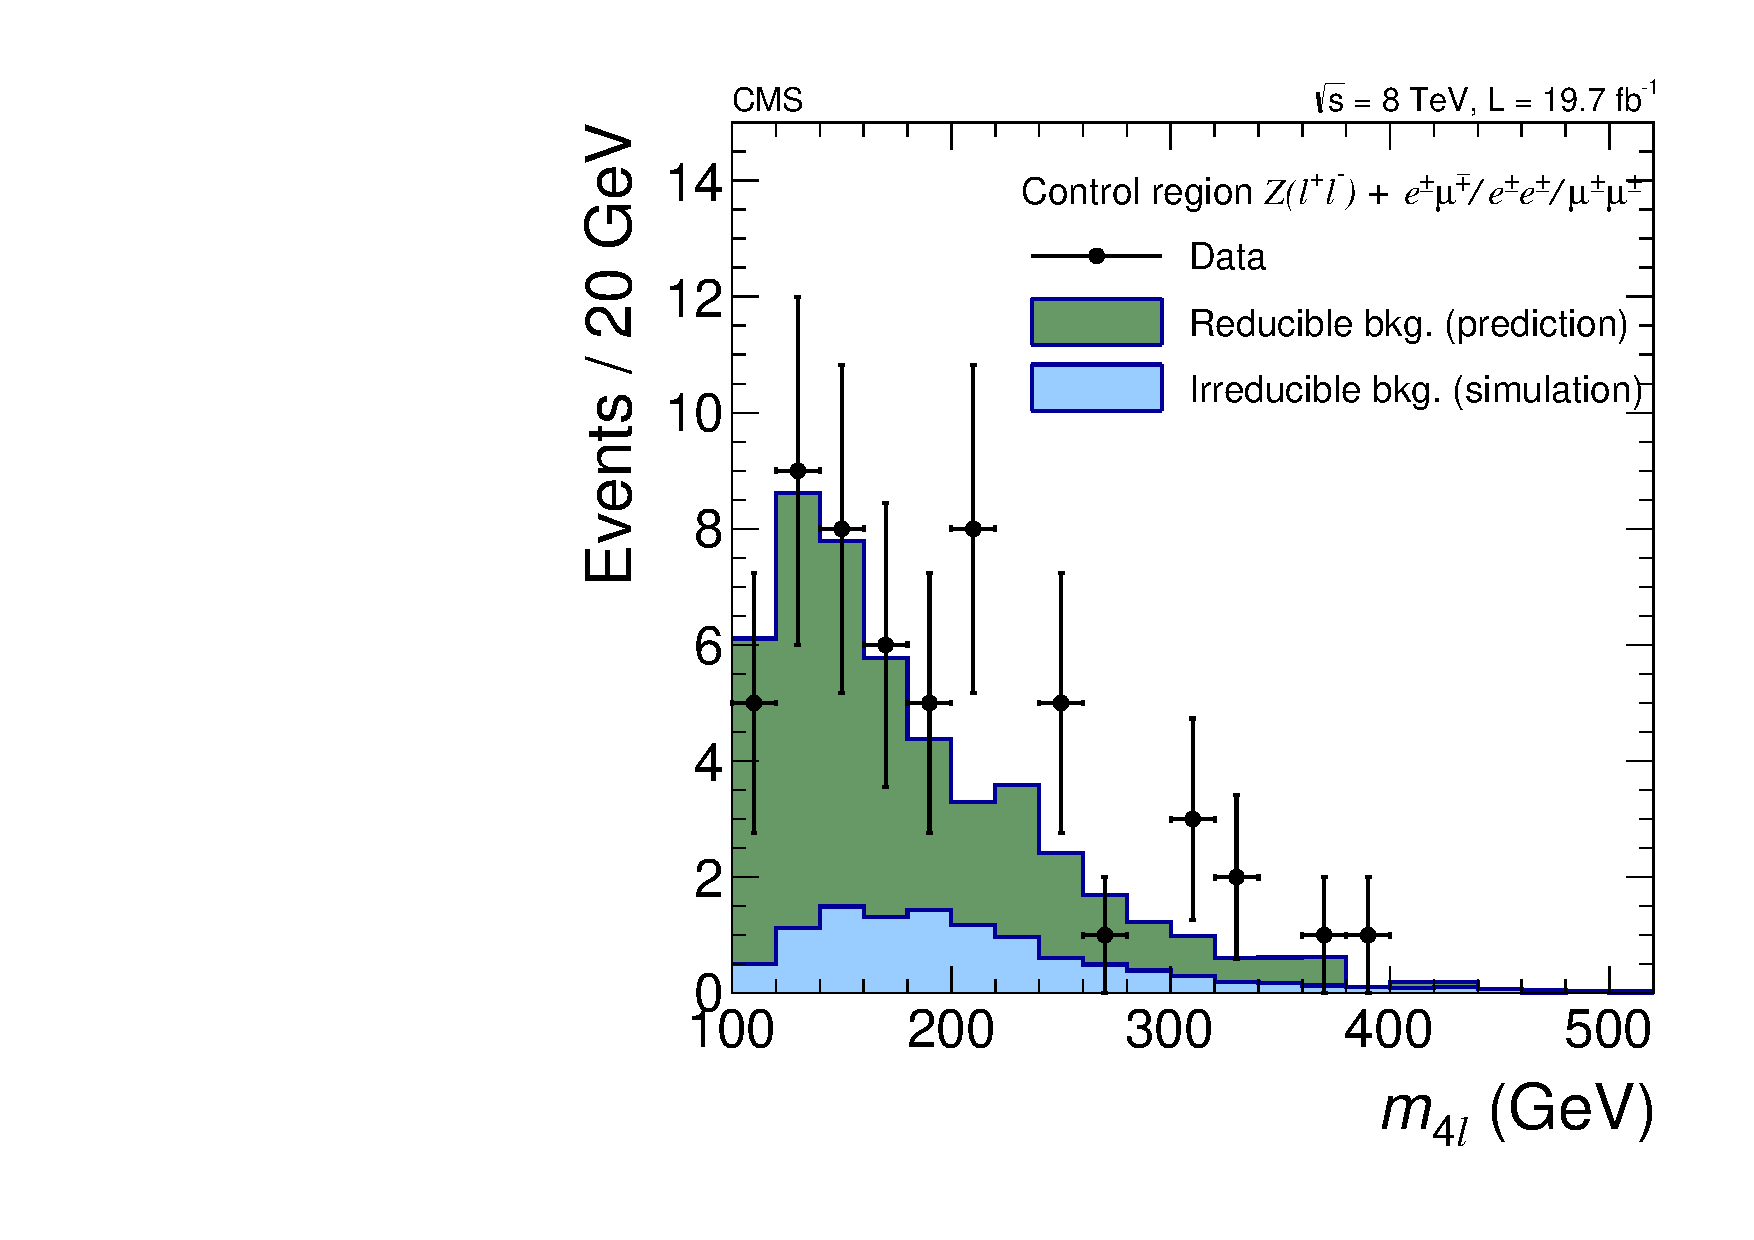
\includegraphics[width=0.45\textwidth]{HZZ4l_search/CRs_m4l_SR_4l_Prediction_WFC_PAPER.pdf}
   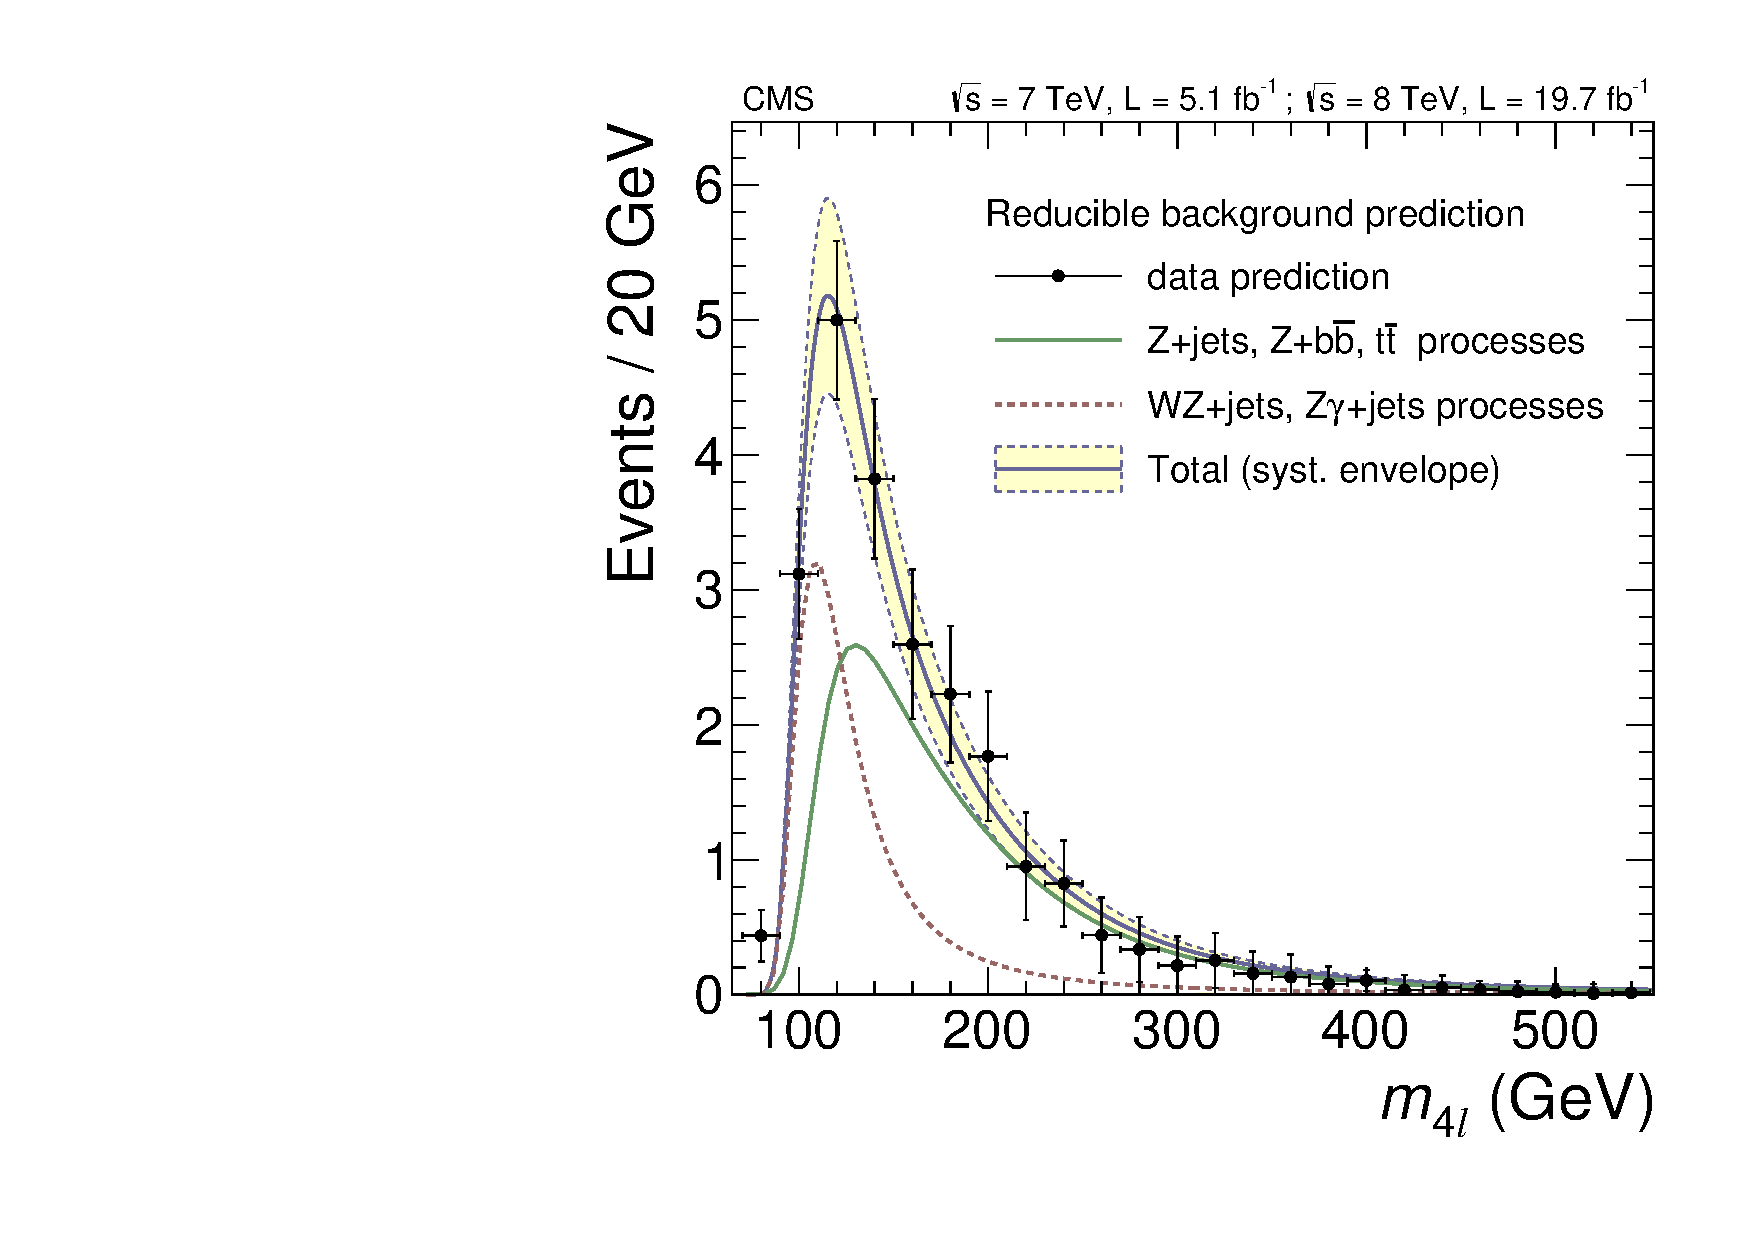
\includegraphics[width=0.45\textwidth]{HZZ4l_search/PredictedComponentsSR_withData_PAPER.pdf}
   \caption[(left) Validation of the method using the SS control
     sample. The observed $m_{4\ell}$ distribution (black dots),
     prediction of the reducible background (dark green area), and
     expected contributions from $ZZ$ (light blue area) are
     shown. (right) Prediction for the reducible background in all three
     decay channels together (black dots) fitted using an empirical shape
     (blue curve) with indicated total uncertainty (yellow band). The
     contributions from the 2P2F-like (solid green) and 3P1F-like
     (dashed red) processes are fitted separately.]{(left) Validation of the method using the SS control
     sample. The observed $m_{4\ell}$ distribution (black dots),
     prediction of the reducible background (dark green area), and
     expected contributions from $ZZ$ (light blue area) are
     shown. (right) Prediction for the reducible background in all three
     decay channels together (black dots) fitted using an empirical shape
     (blue curve) with indicated total uncertainty (yellow band). The
     contributions from the 2P2F-like (solid green) and 3P1F-like
     (dashed red) processes are fitted separately \cite{Chatrchyan:2013mxa}.
 \label{fig:zx}}
 \end{center}
 \end{figure}
 
 After all of this simulation, extrapolation, and calculation we can estimate the number of collision events we would expect to observe for the SM backgrounds and for the Higgs boson under different mass hypotheses. In the full analysis region $m_{4\ell} > \unit{100}{\GeV}$ these estimations and the statistical and systematic uncertainty on them is shown in table \ref{tab:PreFitYields}. 
 
 \begin{table}
  \begin{center}
    \caption[The number of observed candidate events compared to the
      mean expected background and signal rates for each final state.
      Uncertainties include statistical and systematic sources.  The results
      are given integrated over the full mass measurement range $m_{4\ell} >
      \unit{100}{\GeV}$ and for 7 and $\unit{8}{\TeV}$ data combined.]{The number of observed candidate events compared to the
      mean expected background and signal rates for each final state.
      Uncertainties include statistical and systematic sources.  The results
      are given integrated over the full mass measurement range $m_{4\ell} >
      \unit{100}{\GeV}$ and for 7 and $\unit{8}{\TeV}$ data combined \cite{Chatrchyan:2013mxa}.}
      \label{tab:PreFitYields}
    \begin{tabular}{lccc|c}

      Decay Channel         & $4e$ & $2e2\mu$ & $4\mu$ & $4\ell$  \\
      \hline
      $ZZ$ background  & 77  $\pm$ 10    &  191  $\pm$  25  & 119  $\pm$  15     &  387  $\pm$ 31\\
      $Z + \text{jets}$  background & 7.4 $\pm$ 1.5   & 11.5  $\pm$ 2.9  & 3.6  $\pm$ 1.5     &  22.6 $\pm$ 3.6  \\
      \hline
      All backgrounds        & 85 $\pm$ 11     & 202  $\pm$ 25    &  123  $\pm$ 15     &  410 $\pm$ 31 \\
      \hline
      $m_{H} =  \unit{500}{\GeV}$ &  5.2  $\pm$  0.6  & 12.2  $\pm$  1.4 &   7.1  $\pm$  0.8  &  24.5 $\pm$ 1.7  \\
      $m_{H} =  \unit{800}{\GeV}$ &  0.7  $\pm$  0.1  &  1.6  $\pm$  0.2 &   0.9  $\pm$  0.1  &  3.1  $\pm$ 0.2 \\
      \hline
      Observed  & 89 & 247 & 134 & 470\\
    \end{tabular}
  \end{center}
\end{table}


\section{Kinematic Distributions}
\label{sec:Kin_Dists}

Beyond counting the number of observed and expected collision events within the signal region, this analysis utilizes three kinematic distributions to separate potential signal events from background SM production. The first is the $m_{4\ell}$ shape, second is a kiematic discriminanat based on the matrix elements of both signal and background processes, the third is either the $p_{T}^{4\ell}$ or jet kinematic discriminant depending on the number of jets observed in addition to the four leptons.

\subsection{$4\ell$ mass spectrum}
\label{sec:m4l_spectrum}

The background from $ZZ$ and $Z + \text{jets}$ processes dominates after the event selection. The reconstructed four-lepton invariant mass distribution for the combined $4e, 2e2\mu,\text{ and }4\mu$ channels is shown in figure \ref{fig:Mass4l} and compared with the expectations from background processes.

\begin{figure}
\centering

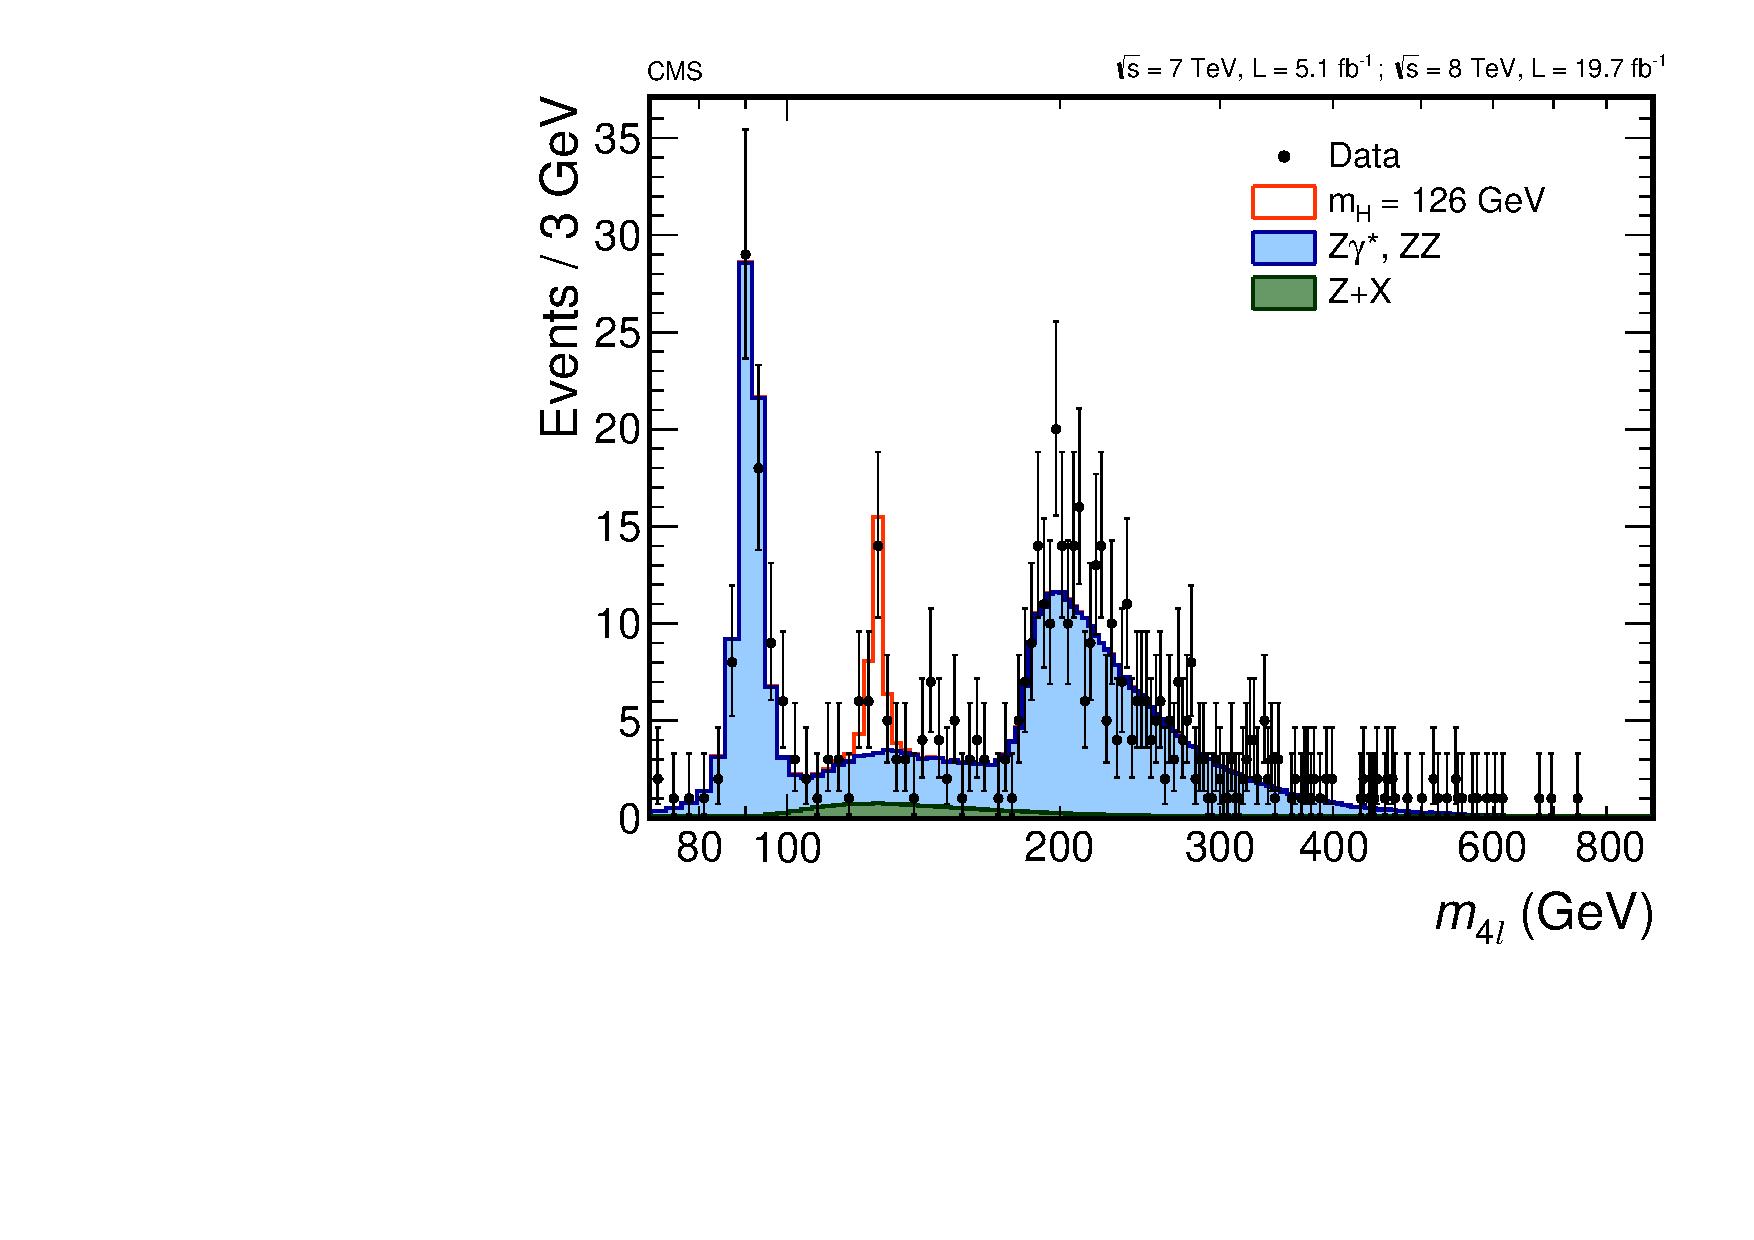
\includegraphics[width=\linewidth]{HZZ4l_search/ZZMass_7Plus8TeV_70-1000_3GeV.pdf}
\caption[Distribution of the four-lepton reconstructed mass in the
  full mass range $70<m_{4\ell}<\unit{1000}{\GeV}$ for the sum of the $4e$,
  $2e2\mu$, and $4\mu$ channels.  Points with error bars represent
  the data, shaded histograms represent the backgrounds, and the
  unshaded histogram represents the signal expectation for a mass
  hypothesis of $m_{H} = \unit{126}{\GeV}$. Signal and the $ZZ$ background are
  normalized to the SM expectation; the $Z+\text{jets}$ background to the
  estimation from data.  The expected distributions are presented as
  stacked histograms. No events are observed with
  $m_{4\ell}>\unit{800}{\GeV}$.]{ Distribution of the four-lepton reconstructed mass in the
  full mass range $70<m_{4\ell}<\unit{1000}{\GeV}$ for the sum of the $4e$,
  $2e2\mu$, and $4\mu$ channels.  Points with error bars represent
  the data, shaded histograms represent the backgrounds, and the
  unshaded histogram represents the signal expectation for a mass
  hypothesis of $m_{H} = \unit{126}{\GeV}$. Signal and the $ZZ$ background are
  normalized to the SM expectation; the $Z+\text{jets}$ background to the
  estimation from data.  The expected distributions are presented as
  stacked histograms. No events are observed with
  $m_{4\ell}>\unit{800}{\GeV}$ \cite{Chatrchyan:2013mxa}.  \label{fig:Mass4l}}

\end{figure}

The normalization and shape of the ZZ background are obtained from simulation, while the normalization of the reducible background is estimated from control samples in data, as described in section \ref{sec:BkgEstimation}. The $m_{4\ell}$ shape of the reducible background component is obtained from the opposite-sign method by fitting the $m_{4\ell}$ distributions of 2P2F and 3P1F regions separately with empirical functional forms built from Landau and exponential distributions. The systematic uncertainty in the shape is determined by the envelope that covers alternative functional forms or alternative binning.

The signal $m_{4\ell}$ shapes are also obtained from simulation. For low-mass Higgs boson hypotheses $\left(m_{H} < \unit{400}{\GeV}\right)$, the Higgs boson line shape is described with a relativistic Breit-Wigner (BW) convolved with a double-sided Crystal-Ball (CB) distribution to parameterize the reconstructed signal $m_{4\ell}$ distributions. The resulting model for the $m_{4\ell}$ peak can be seen in figure \ref{fig:4lmassmc}, where the parameterization for each final state can be seen superimposed on simulated data events. At high mass $\left(m_{H} > \unit{400}{\GeV}\right)$, the line shape is described using the complex pole scheme (CPS) \cite{Passarino:2010qk, Goria:2011wa, Kauer:2012hd}. This results in a Higgs boson width much larger than the four-lepton mass resolution. The signal parameterization for these hypotheses are modified according to this increased width instead of using the double CB functions. Systematics on the line shape are incorporated by varying the signal weights as a function of the Higgs boson mass by $\pm1\sigma$.

\begin{figure}
\centering
     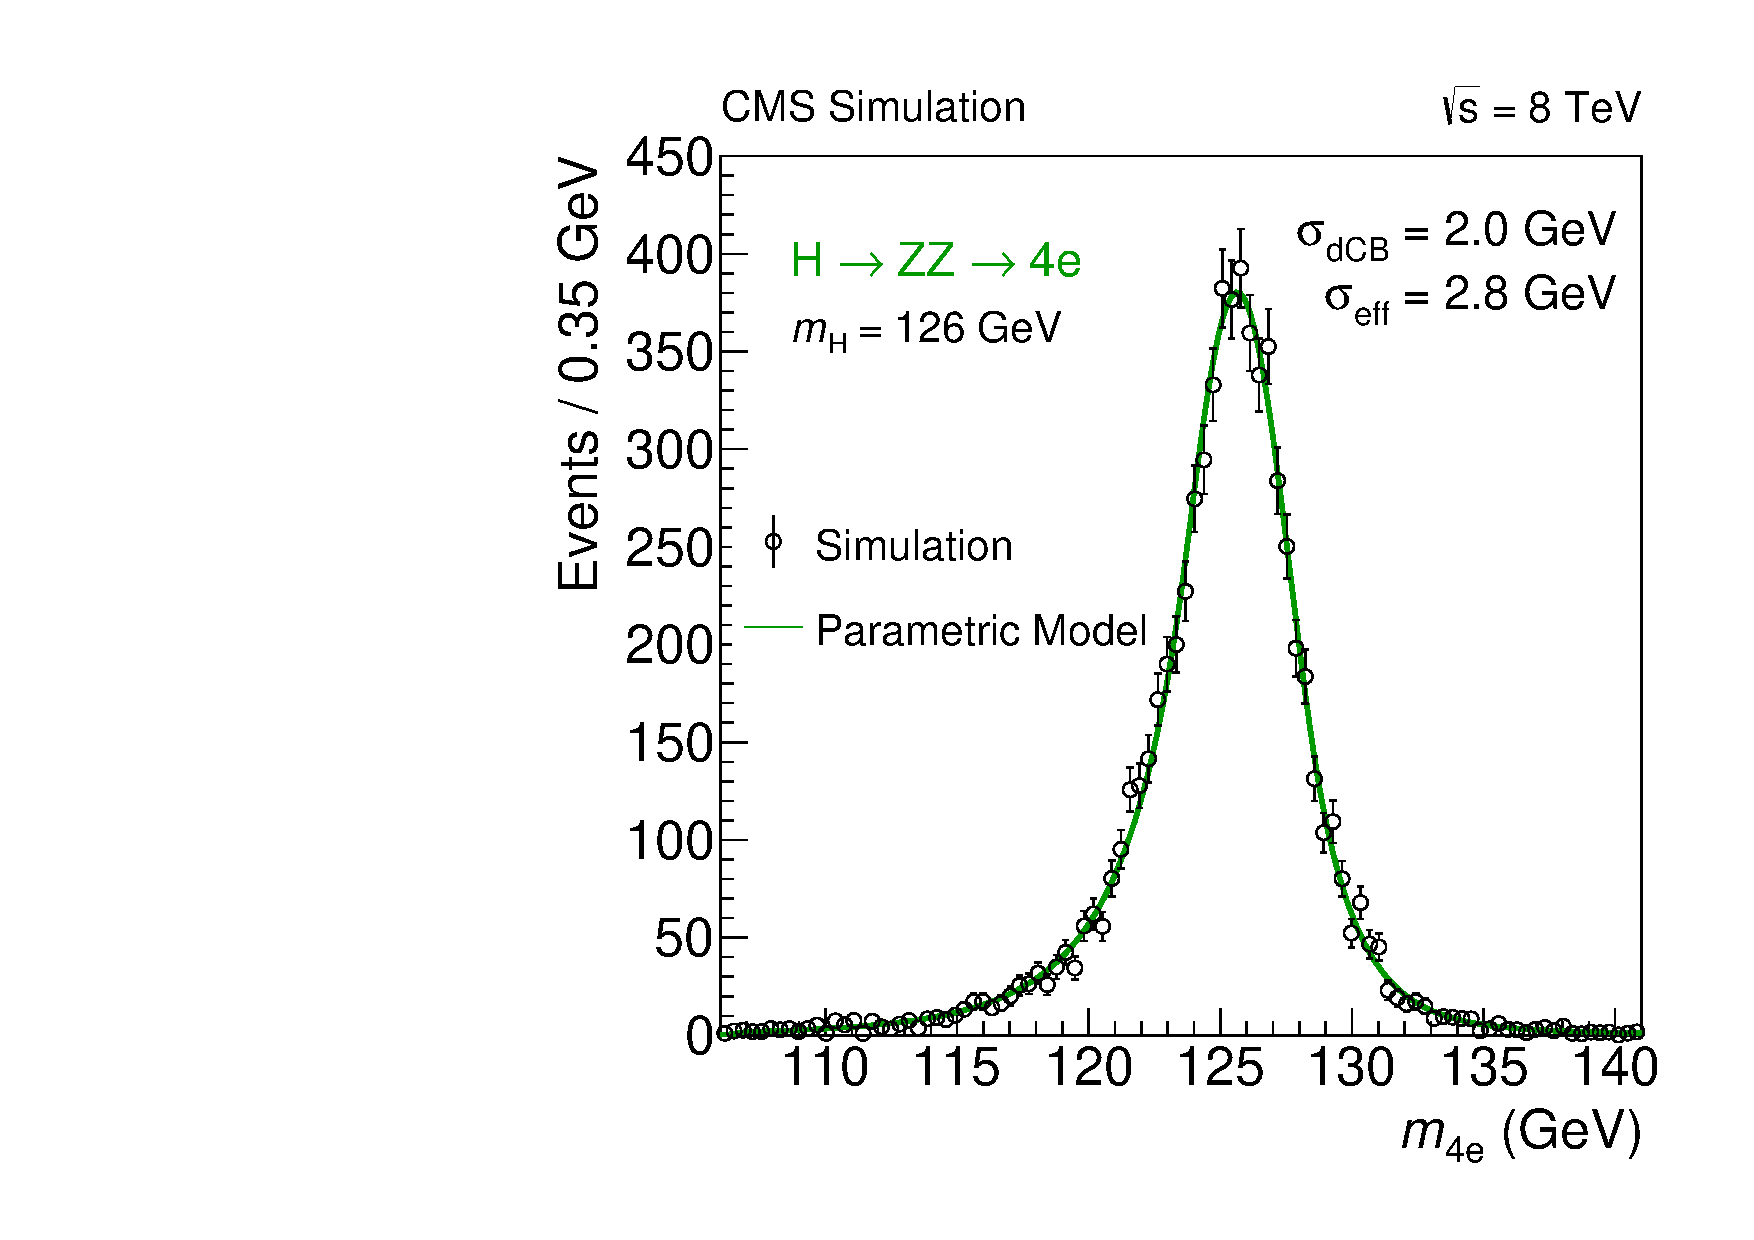
\includegraphics[width=0.32\linewidth]{HZZ4l_search/fitM126_channel1.pdf}
     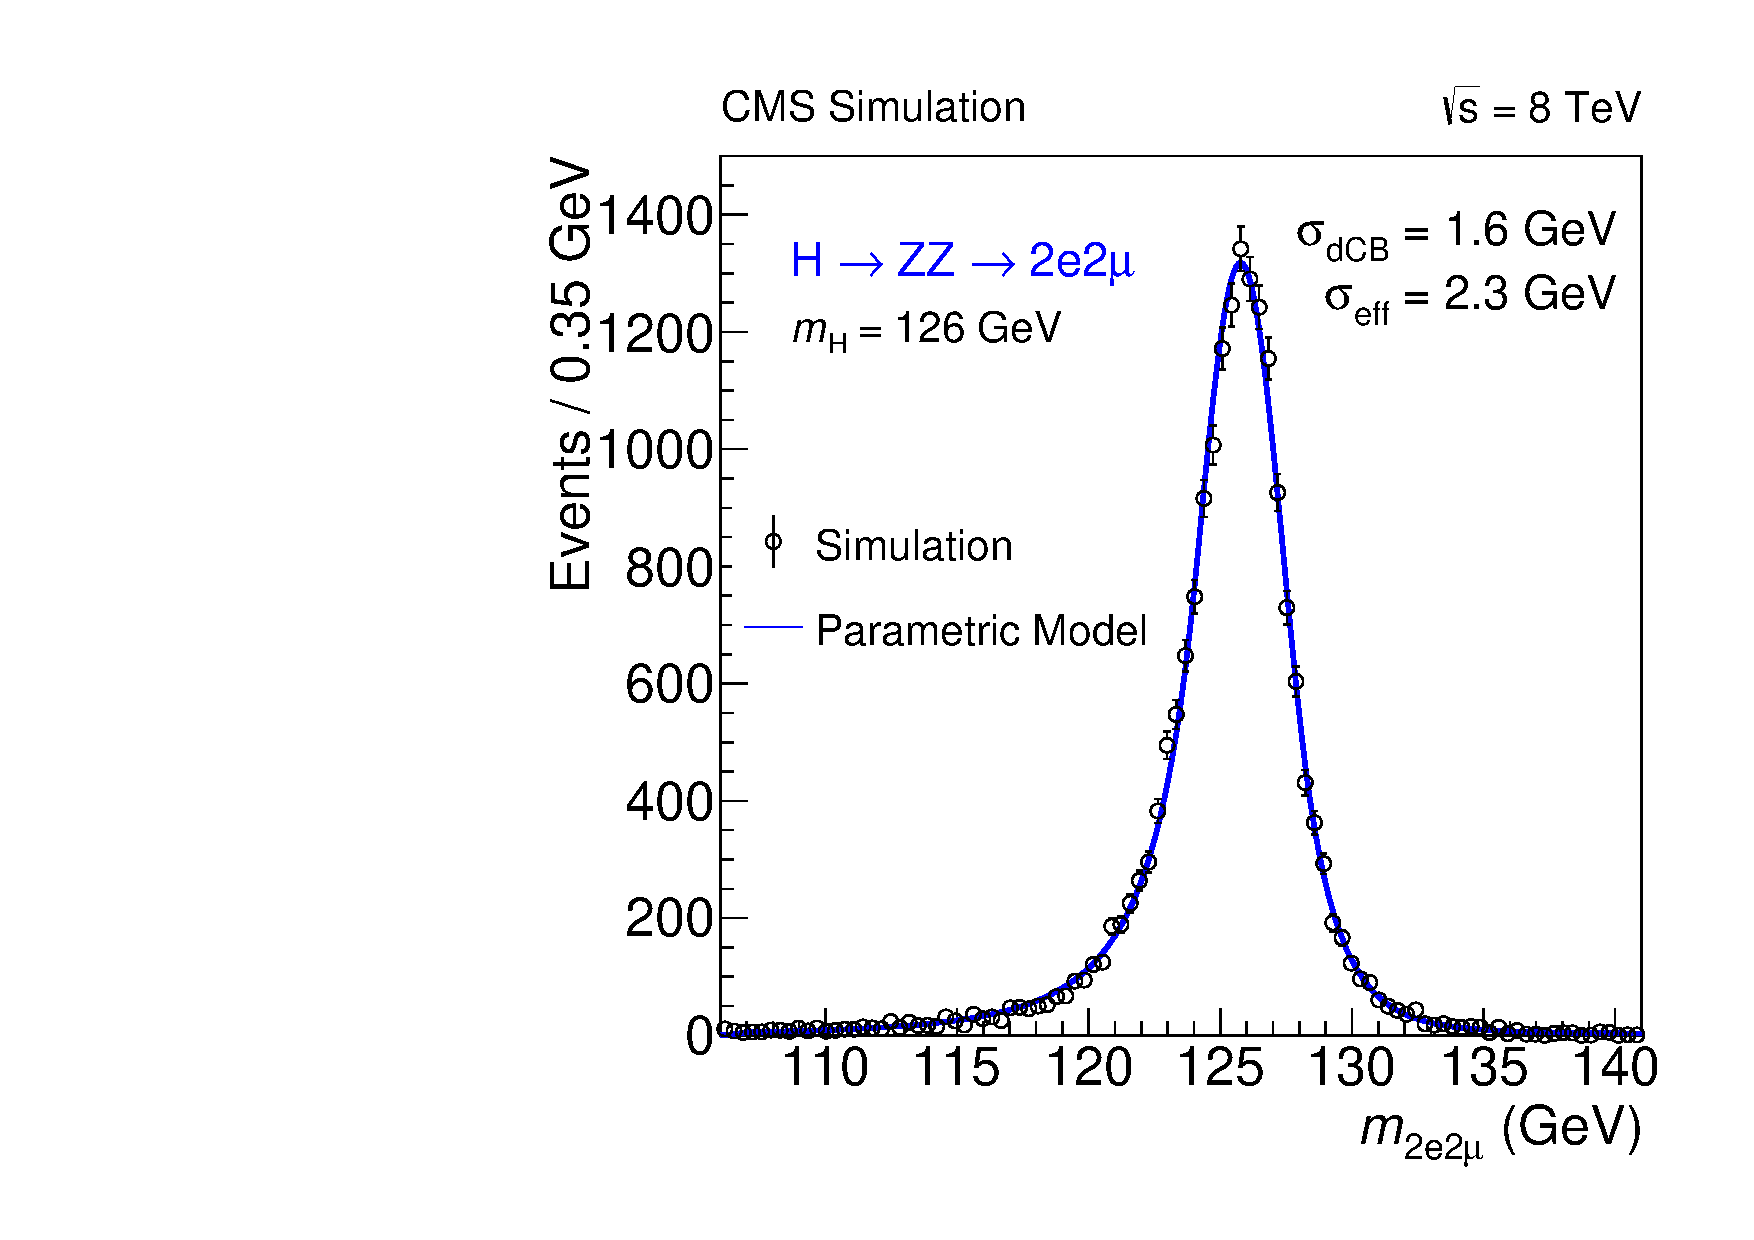
\includegraphics[width=0.32\linewidth]{HZZ4l_search/fitM126_channel2.pdf}
     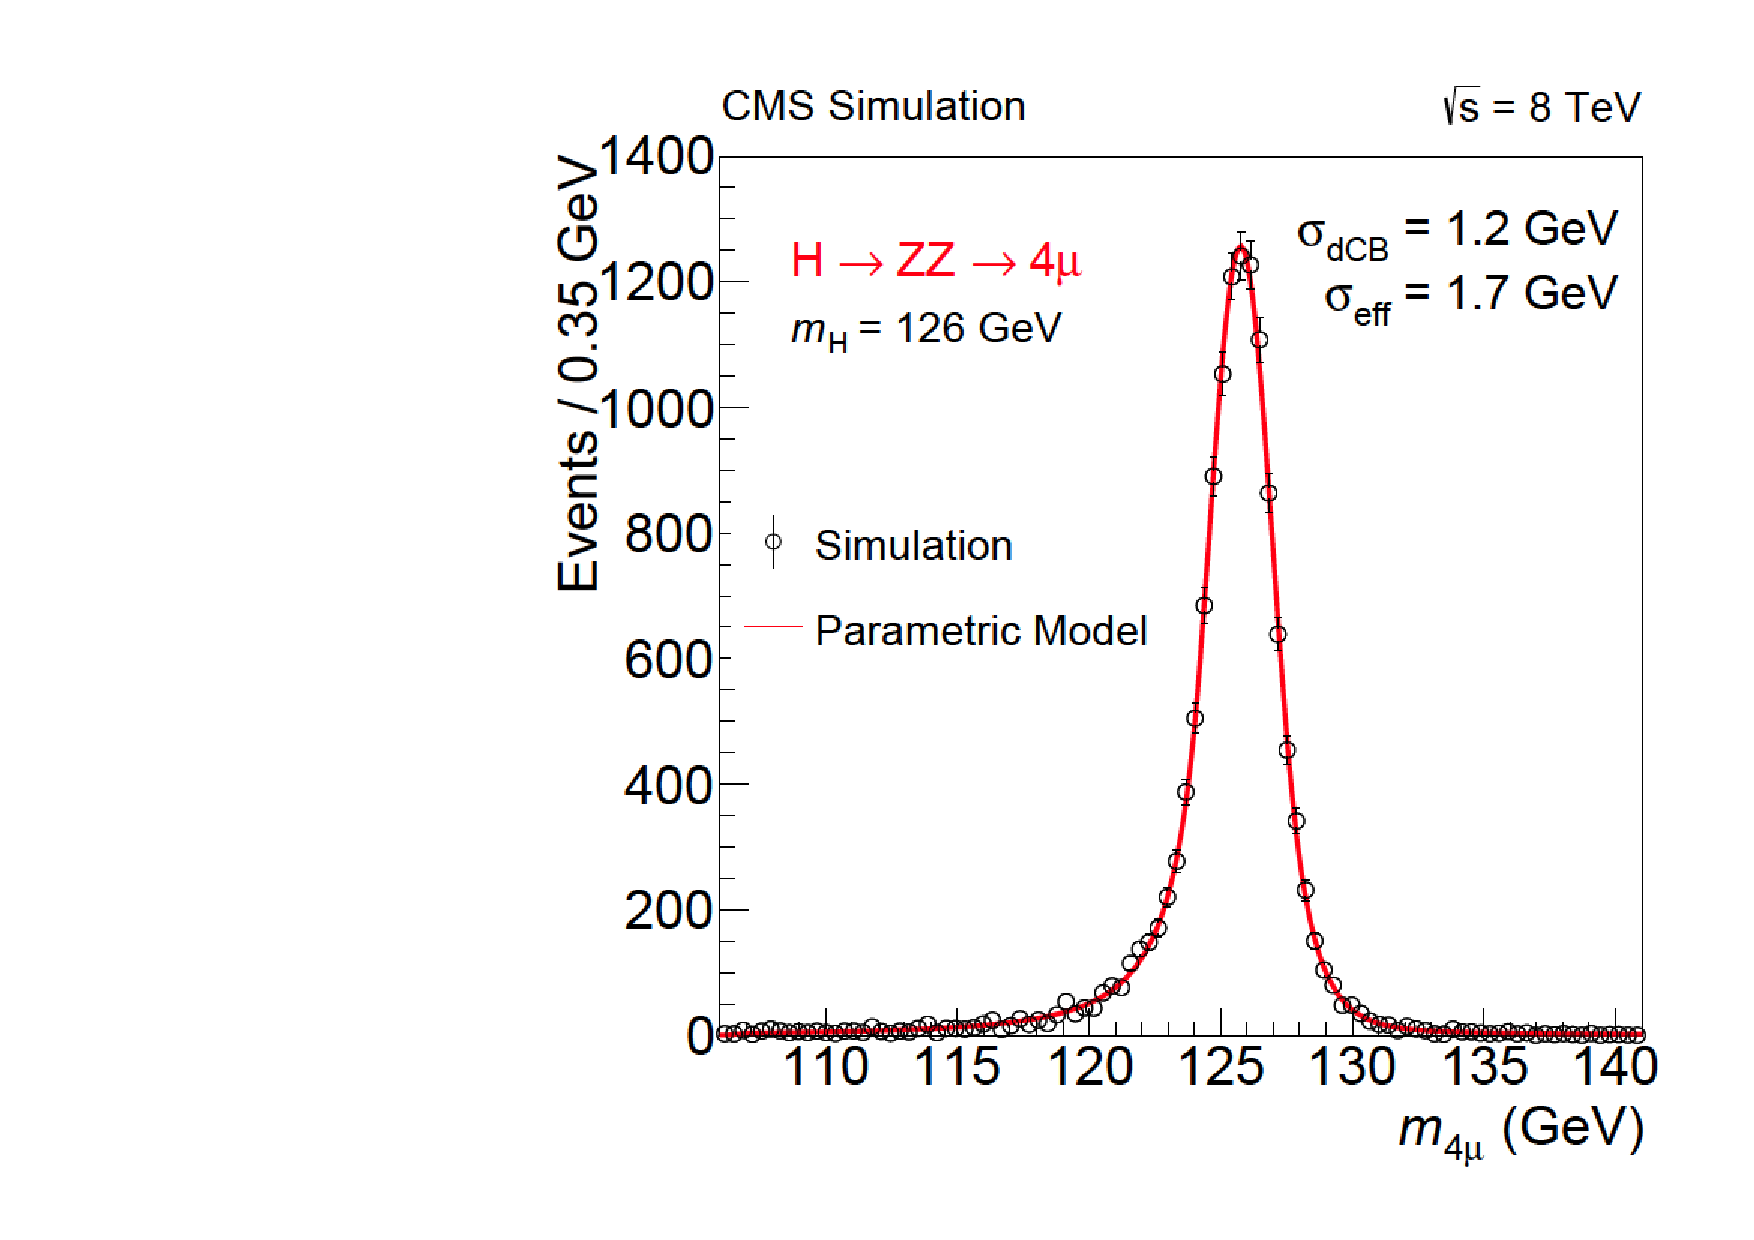
\includegraphics[width=0.32\linewidth]{HZZ4l_search/fitM126_channel0.pdf}
\caption[The $H \to ZZ \to 4\ell$ invariant mass
  distribution for $m_{H} = \unit{126}{\GeV}$ in the (left) $4e$, (center) $2e2\mu$,
  and (right) $4\mu$ channels. The distributions are fitted with a
  double-sided CB function and the fitted values of the CB width
  $\sigma_{\mathrm{dCB}}$ are indicated. The values of effective resolution,
  defined as half the smallest width that contains 68.3\% of the
  distribution, are also indicated. The distributions are arbitrarily
  normalized.]{ The $H \to ZZ \to 4\ell$ invariant mass
  distribution for $m_{H} = \unit{126}{\GeV}$ in the (left) $4e$, (center) $2e2\mu$,
  and (right) $4\mu$ channels. The distributions are fitted with a
  double-sided CB function and the fitted values of the CB width
  $\sigma_{\mathrm{dCB}}$ are indicated. The values of effective resolution,
  defined as half the smallest width that contains 68.3\% of the
  distribution, are also indicated. The distributions are arbitrarily
  normalized \cite{Chatrchyan:2013mxa}.}
\label{fig:4lmassmc}
\end{figure}


\subsection{Matrix Element Likelihood Approach (MELA) kinematic discriminant}
\label{sec:MELA}

As we have mentioned the four-lepton decay mode has the advantage that the kinematics of the Higgs boson and its decay products are all visible in the detector, providing many independent observables that can be used for different purposes. In addition to the invariant mass, the angular distributions for the four leptons and the dilepton pairs invariant masses can be used to further discriminate signal from background, increasing the sensitivity and reducing the statistical uncertainty in the observations.

Five angles $\vec{\Omega} \equiv \left(\theta^{*}, \Phi_{1}, \theta_{1}, \theta_{2}, \Phi\right)$ \cite{Gao:2010qx, Bolognesi:2012mm, Anderson:2013afp, PhysRev.168.1926} seen in figure \ref{fig:decay}  and the invariant masses of the lepton pairs $m_{Z_{1}}$ and $m_{Z_{2}}$, fully describe the kinematic configuration of a four-lepton system in its center-of-mass frame, up to an arbitrary rotation around the beam axis. These observables provide significant discriminating power between signal and background. A matrix-element likelihood approach (MELA) is used to construct a kinematic discriminant related to the decay observables \cite{Chatrchyan:2013lba, Chatrchyan:2012jja}.

\begin{figure}
\begin{center}
\centering
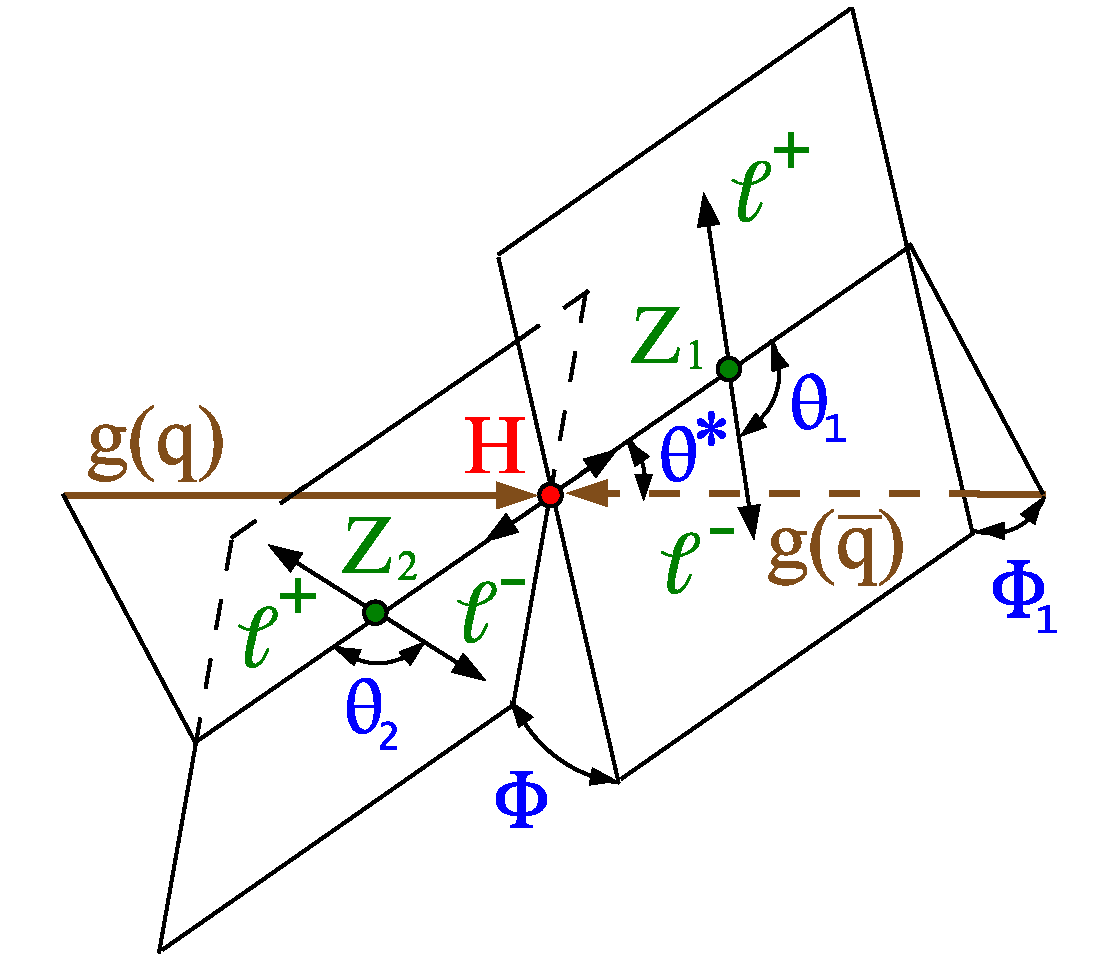
\includegraphics[width=0.45\linewidth]{HZZ4l_search/angles-HZZ4l_snowmass.pdf}
\caption[Illustration of the production and decay of a particle
  $H$, $gg(q\bar{q}) \to H \to ZZ \to 4\ell$, with the two production angles $\theta^*$ and $\Phi_1$ shown
  in the $H$ rest frame and three decay angles $\theta_1$,
  $\theta_2$, and $\Phi$ shown in the $Z_1$, $Z_2$, and $H$
  rest frames, respectively.]{ Illustration of the production and decay of a particle
  $H$, $gg(q\bar{q}) \to H \to ZZ \to 4\ell$, with the two production angles $\theta^*$ and $\Phi_1$ shown
  in the $H$ rest frame and three decay angles $\theta_1$,
  $\theta_2$, and $\Phi$ shown in the $Z_1$, $Z_2$, and $H$
  rest frames, respectively \cite{Anderson:2013afp}.
\label{fig:decay}}
\end{center}
\end{figure}

Each of these five observables carries some information about how the $4\ell$ event was produced. The distribution of these is shown in figure \ref{fig:kinematics}. This figure also shows predicted distributions for BSM bosons, which will become relevant in later sections. In principle, with enough computing power and effort one could construct an analysis that uses all of them independently. However, without loss in performance one can use the event probabilities that come from the matrix-element corresponding to a given point in phase space. This way the analysis is simplified and the correlations between these different variables are maintained.

\begin{figure}
\centering
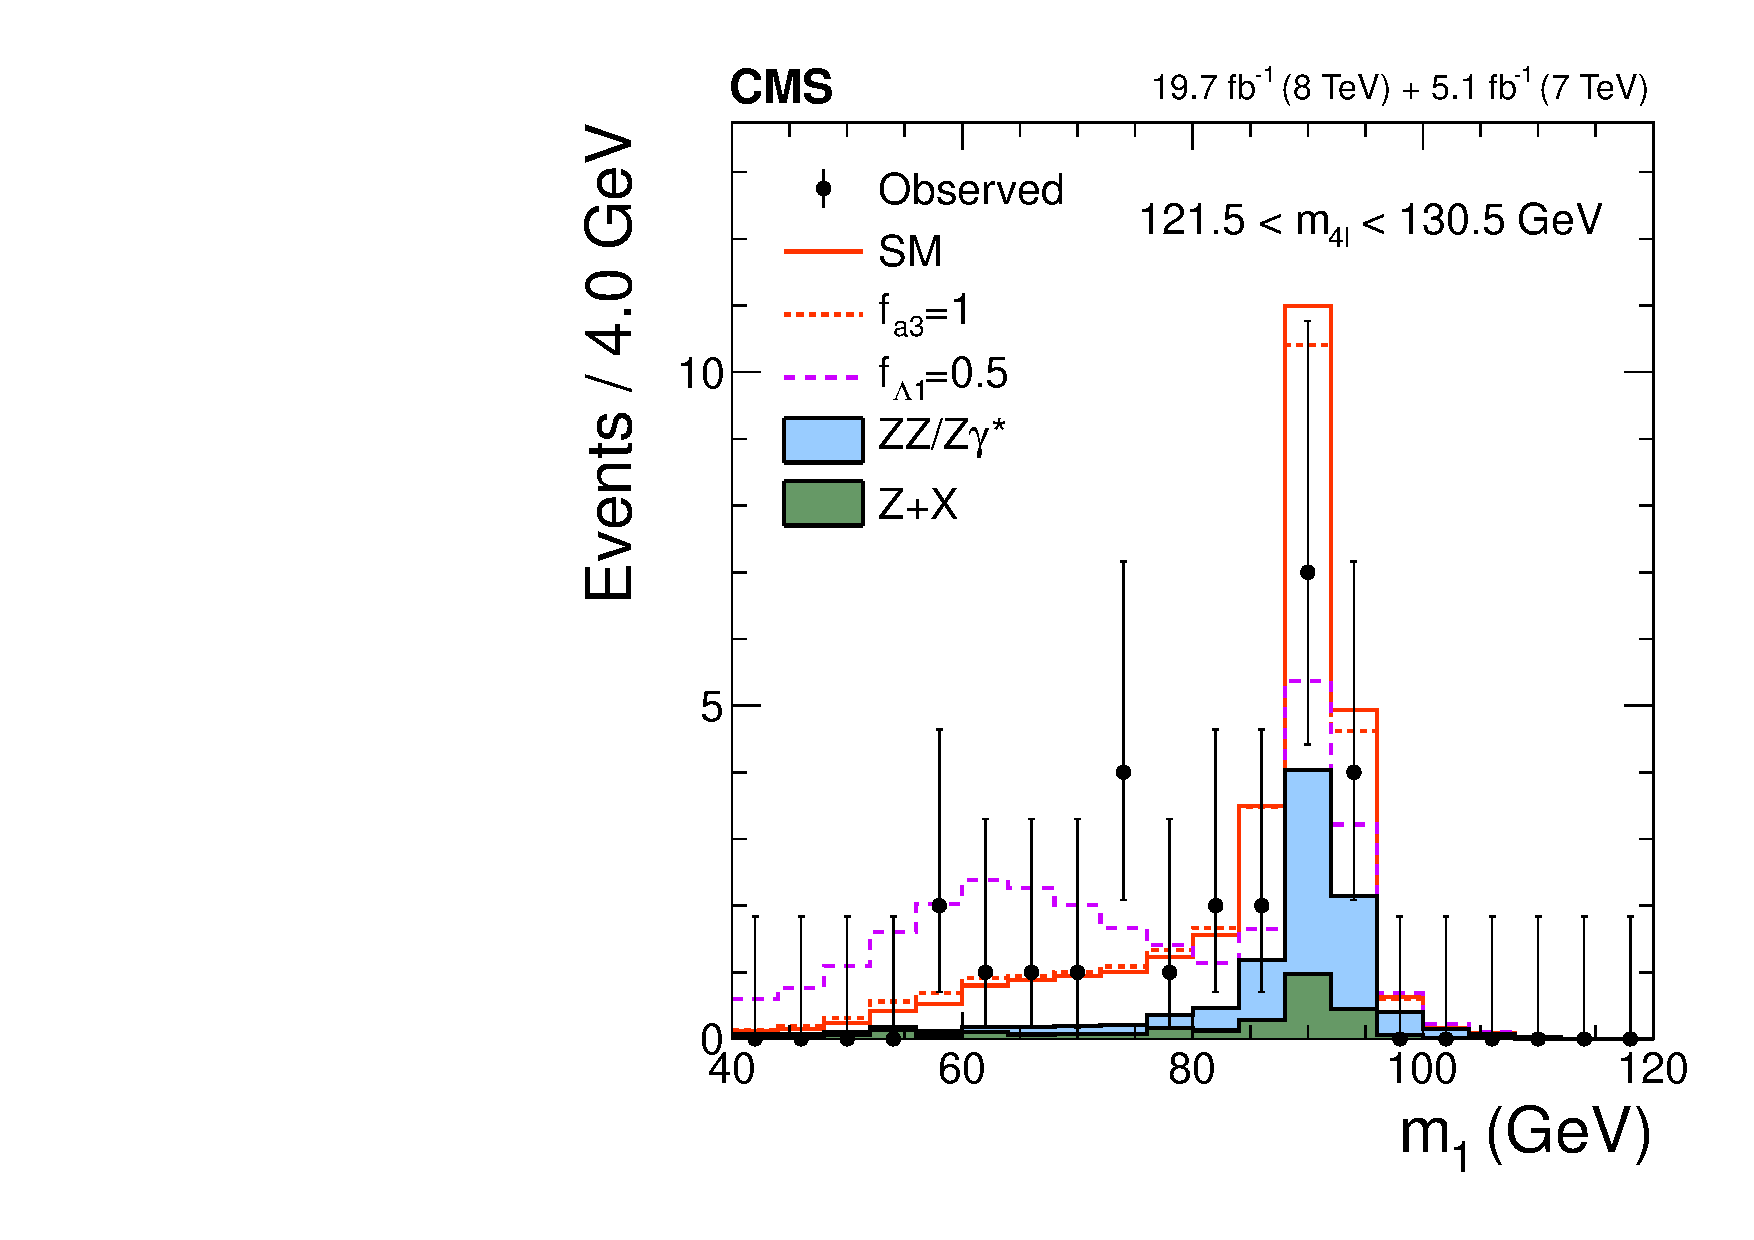
\includegraphics[width=0.32\textwidth]{HZZ4l_search/cCompare_DataMC_AllTeV_Z1Mass_SignalEnriched.pdf}
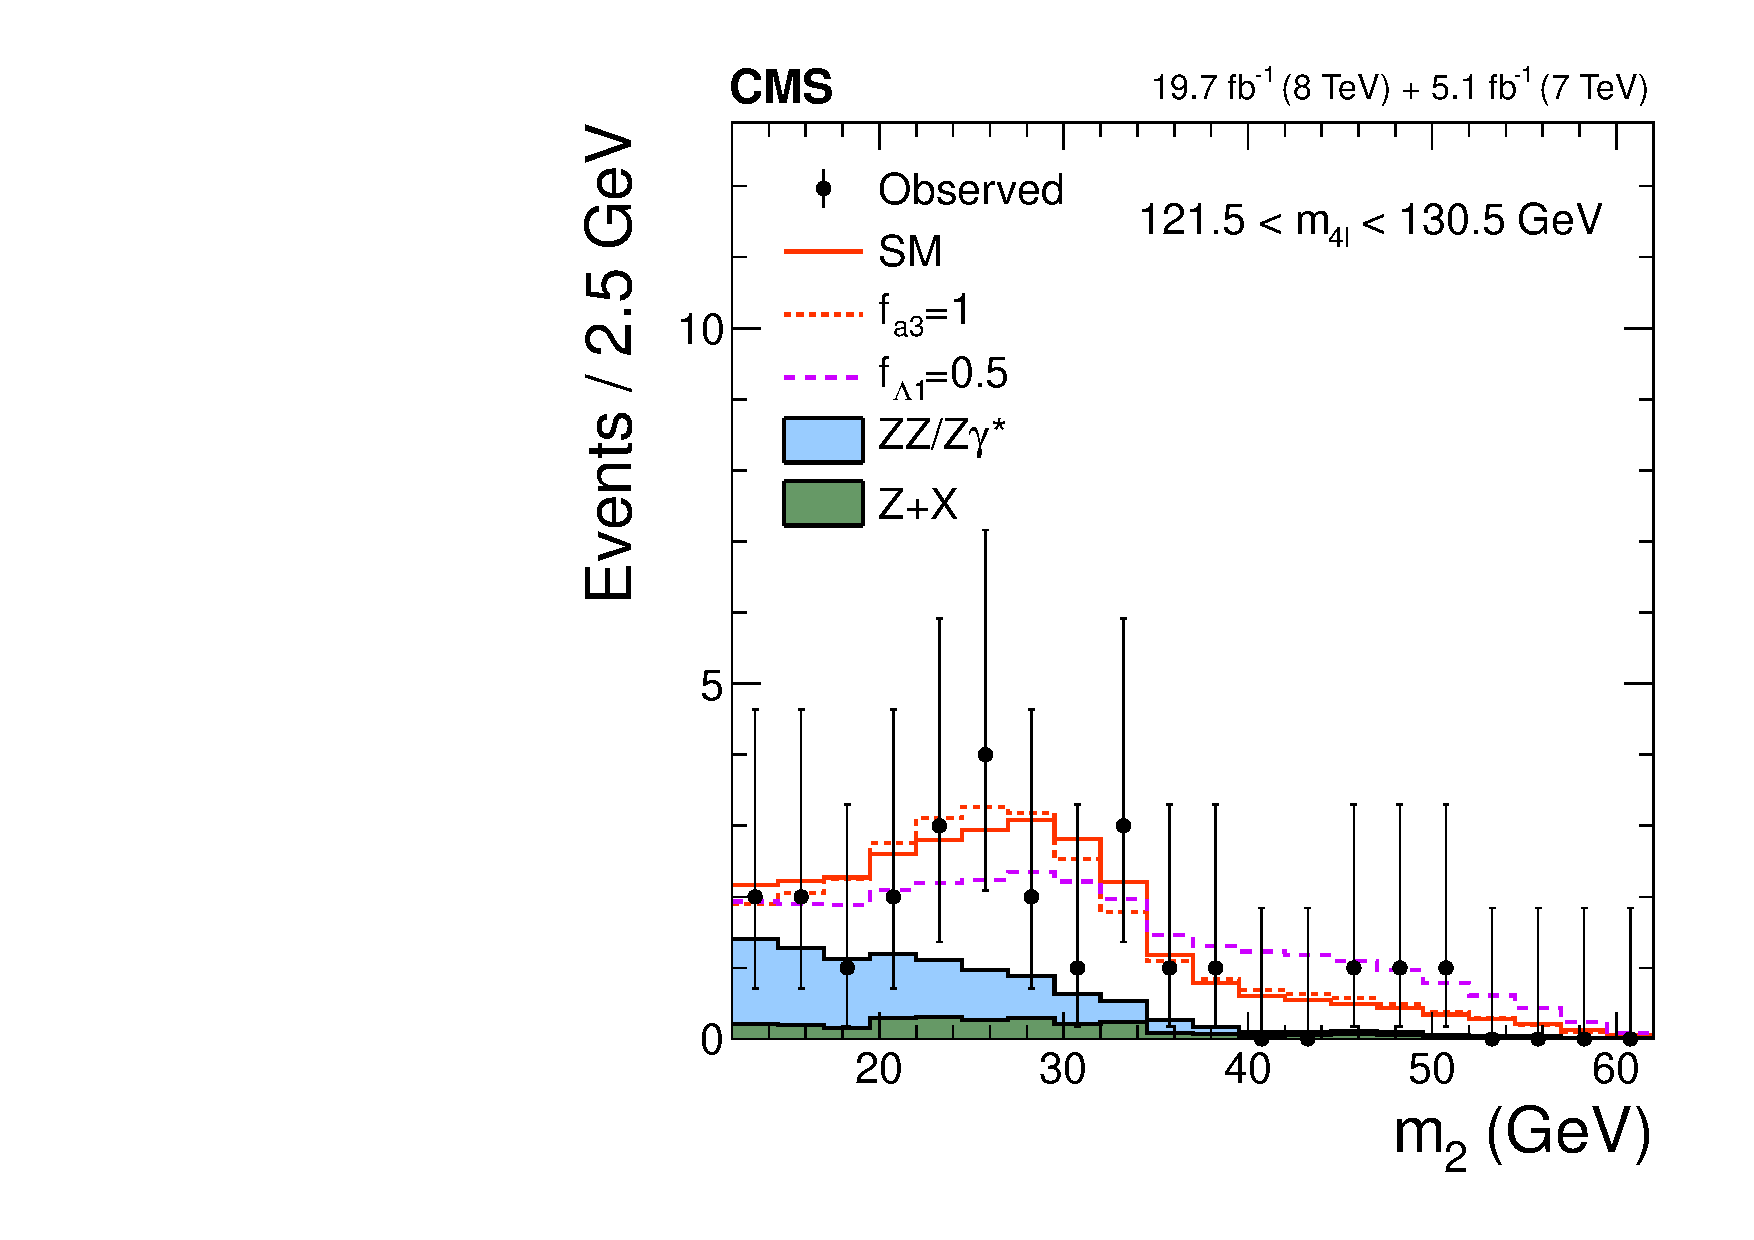
\includegraphics[width=0.32\textwidth]{HZZ4l_search/cCompare_DataMC_AllTeV_Z2Mass_SignalEnriched.pdf} \\
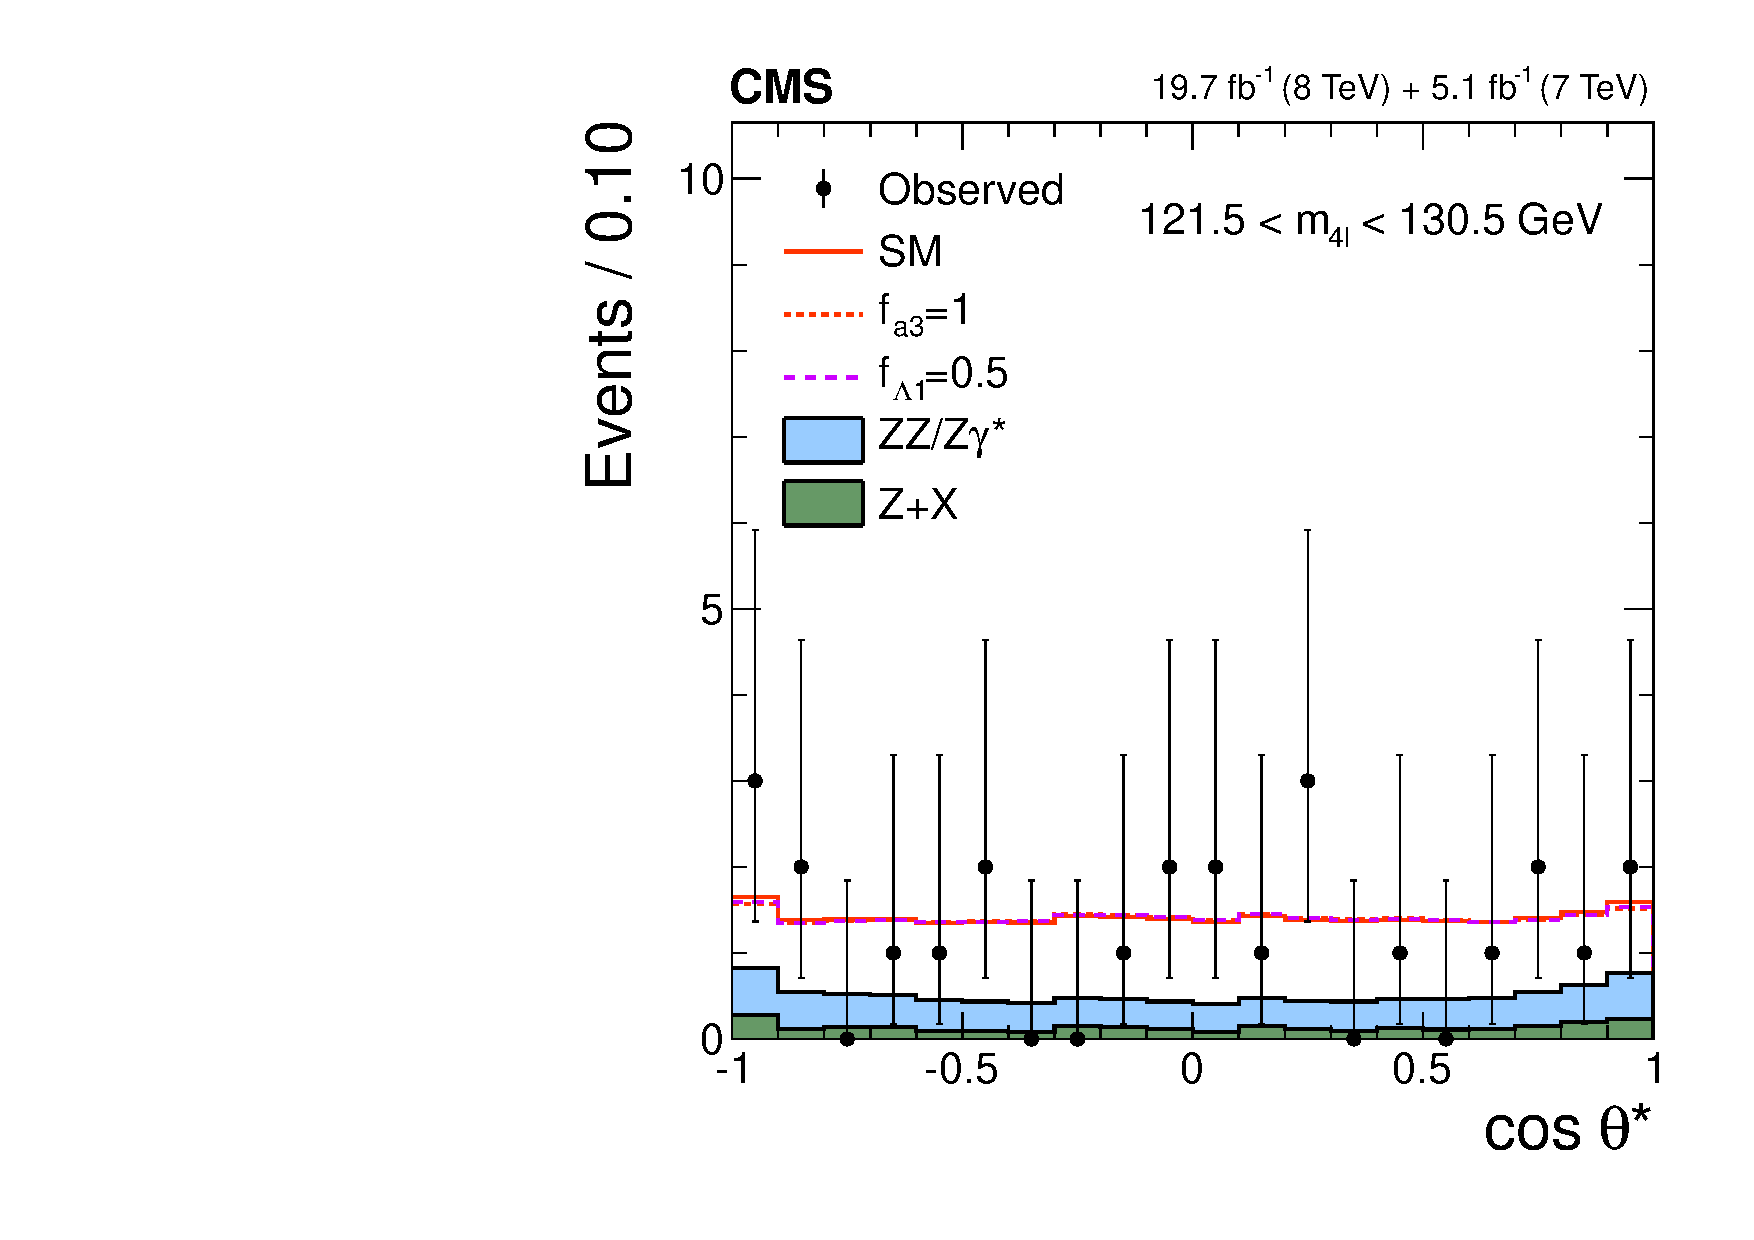
\includegraphics[width=0.32\textwidth]{HZZ4l_search/cCompare_DataMC_AllTeV_costhetastar_SignalEnriched.pdf}
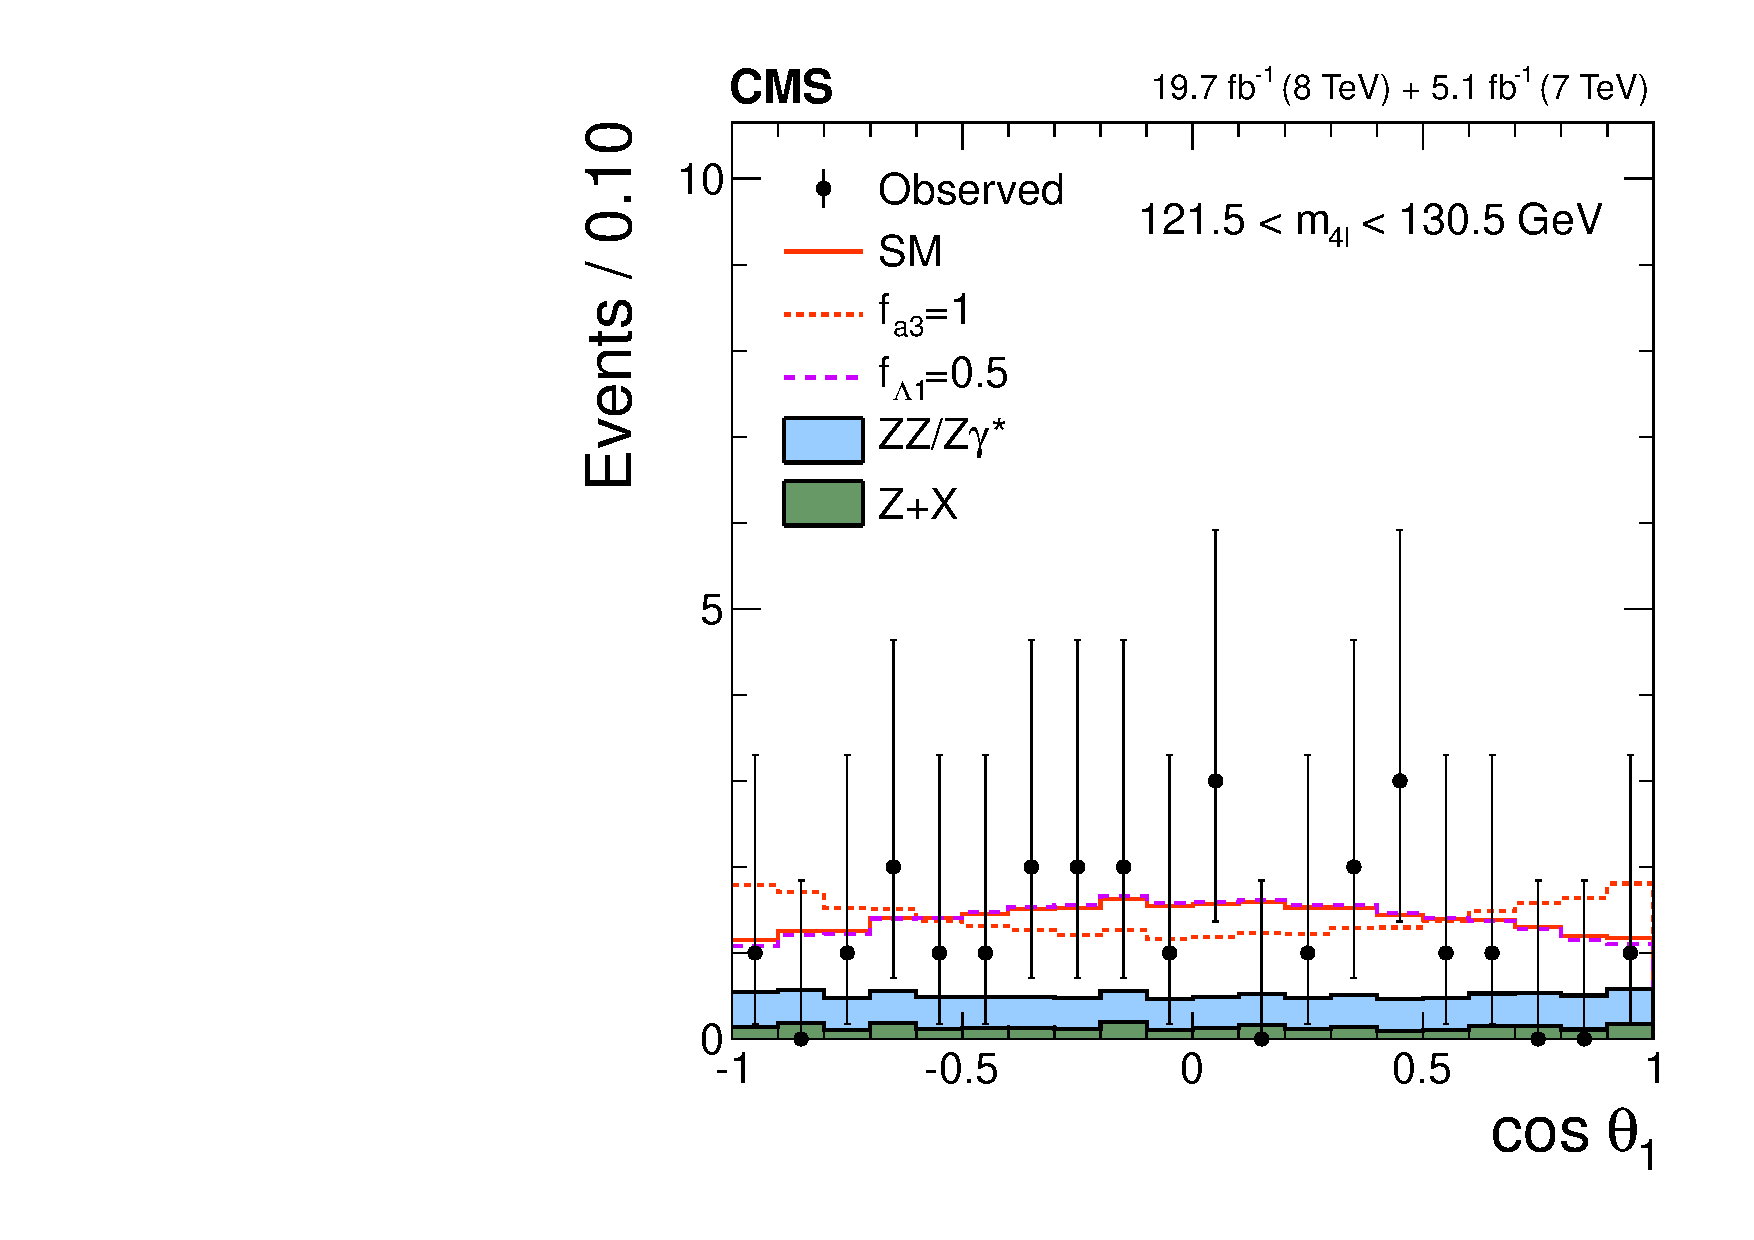
\includegraphics[width=0.32\textwidth]{HZZ4l_search/cCompare_DataMC_AllTeV_helcosthetaZ1_SignalEnriched.pdf}
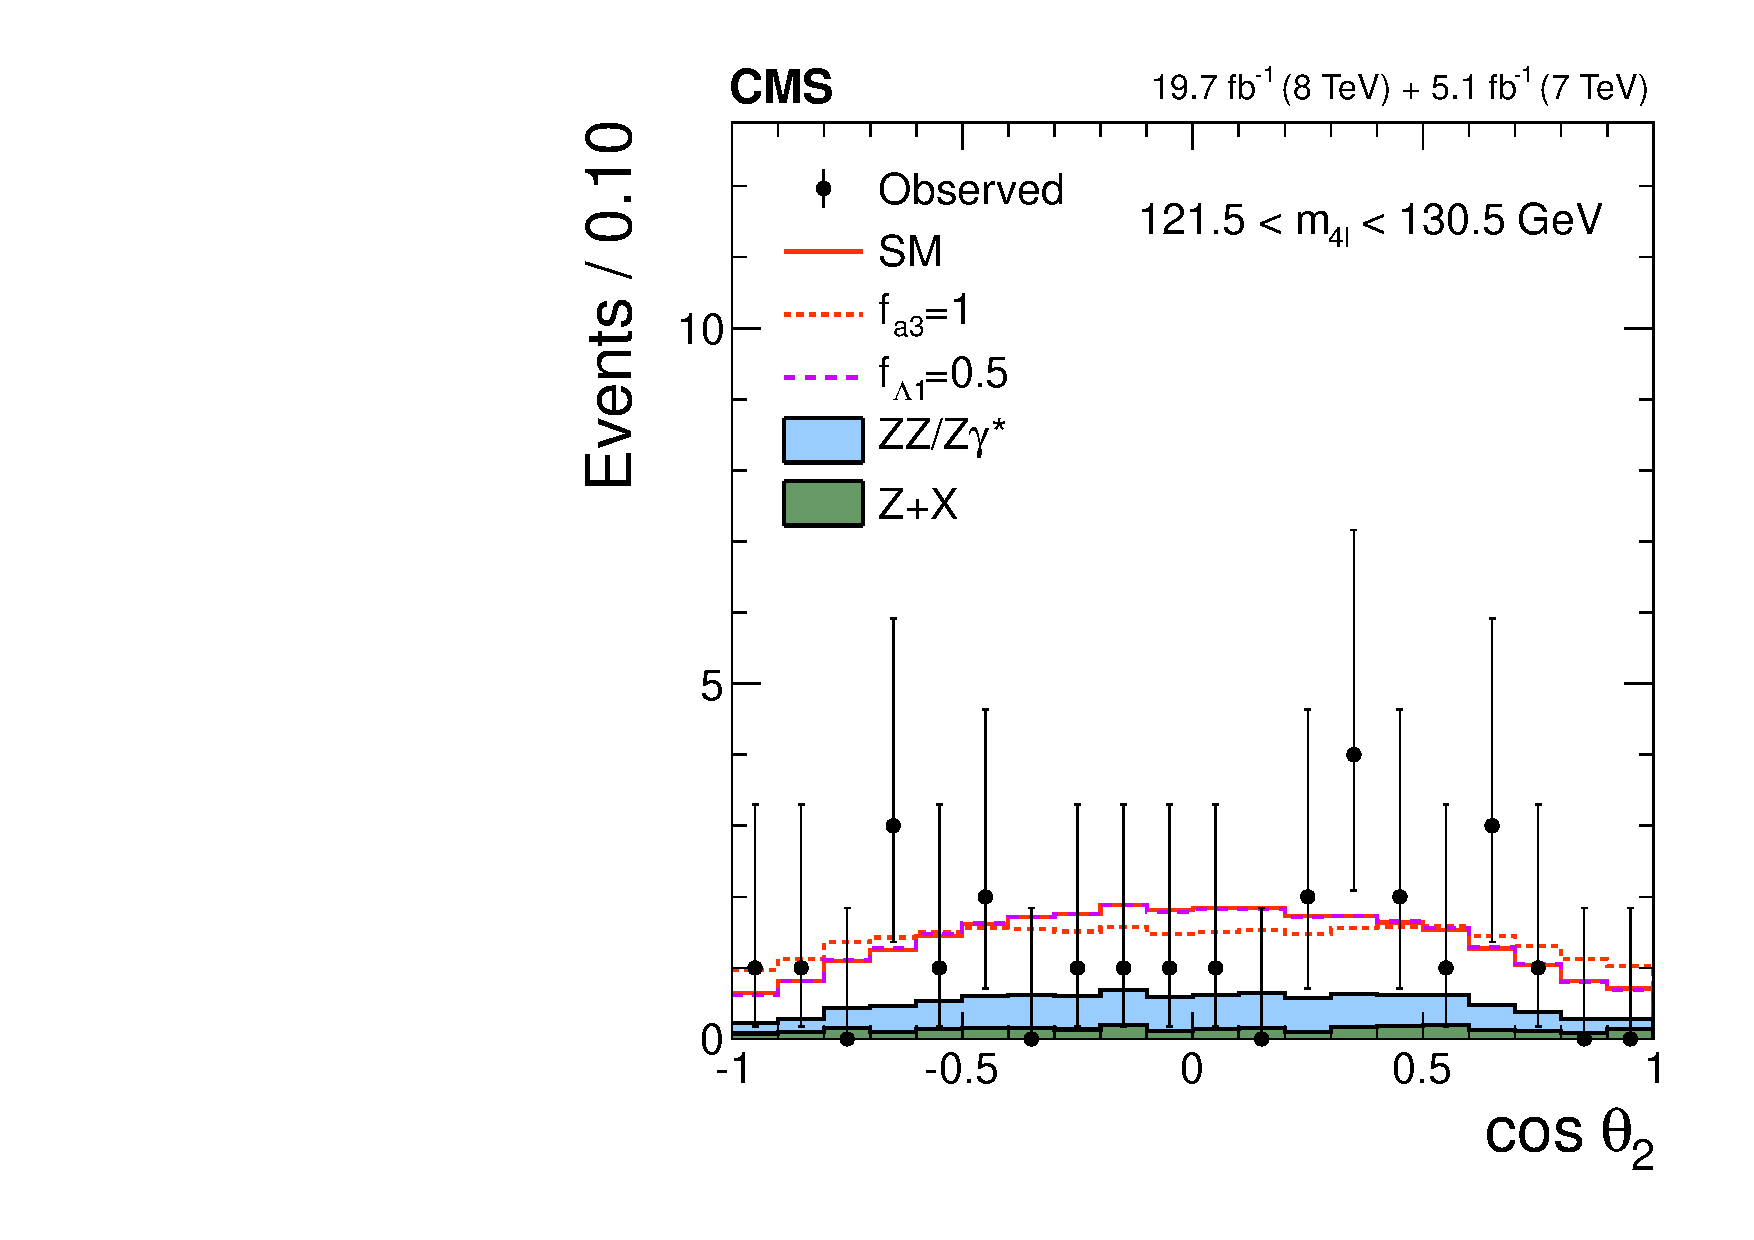
\includegraphics[width=0.32\textwidth]{HZZ4l_search/cCompare_DataMC_AllTeV_helcosthetaZ2_SignalEnriched.pdf} \\
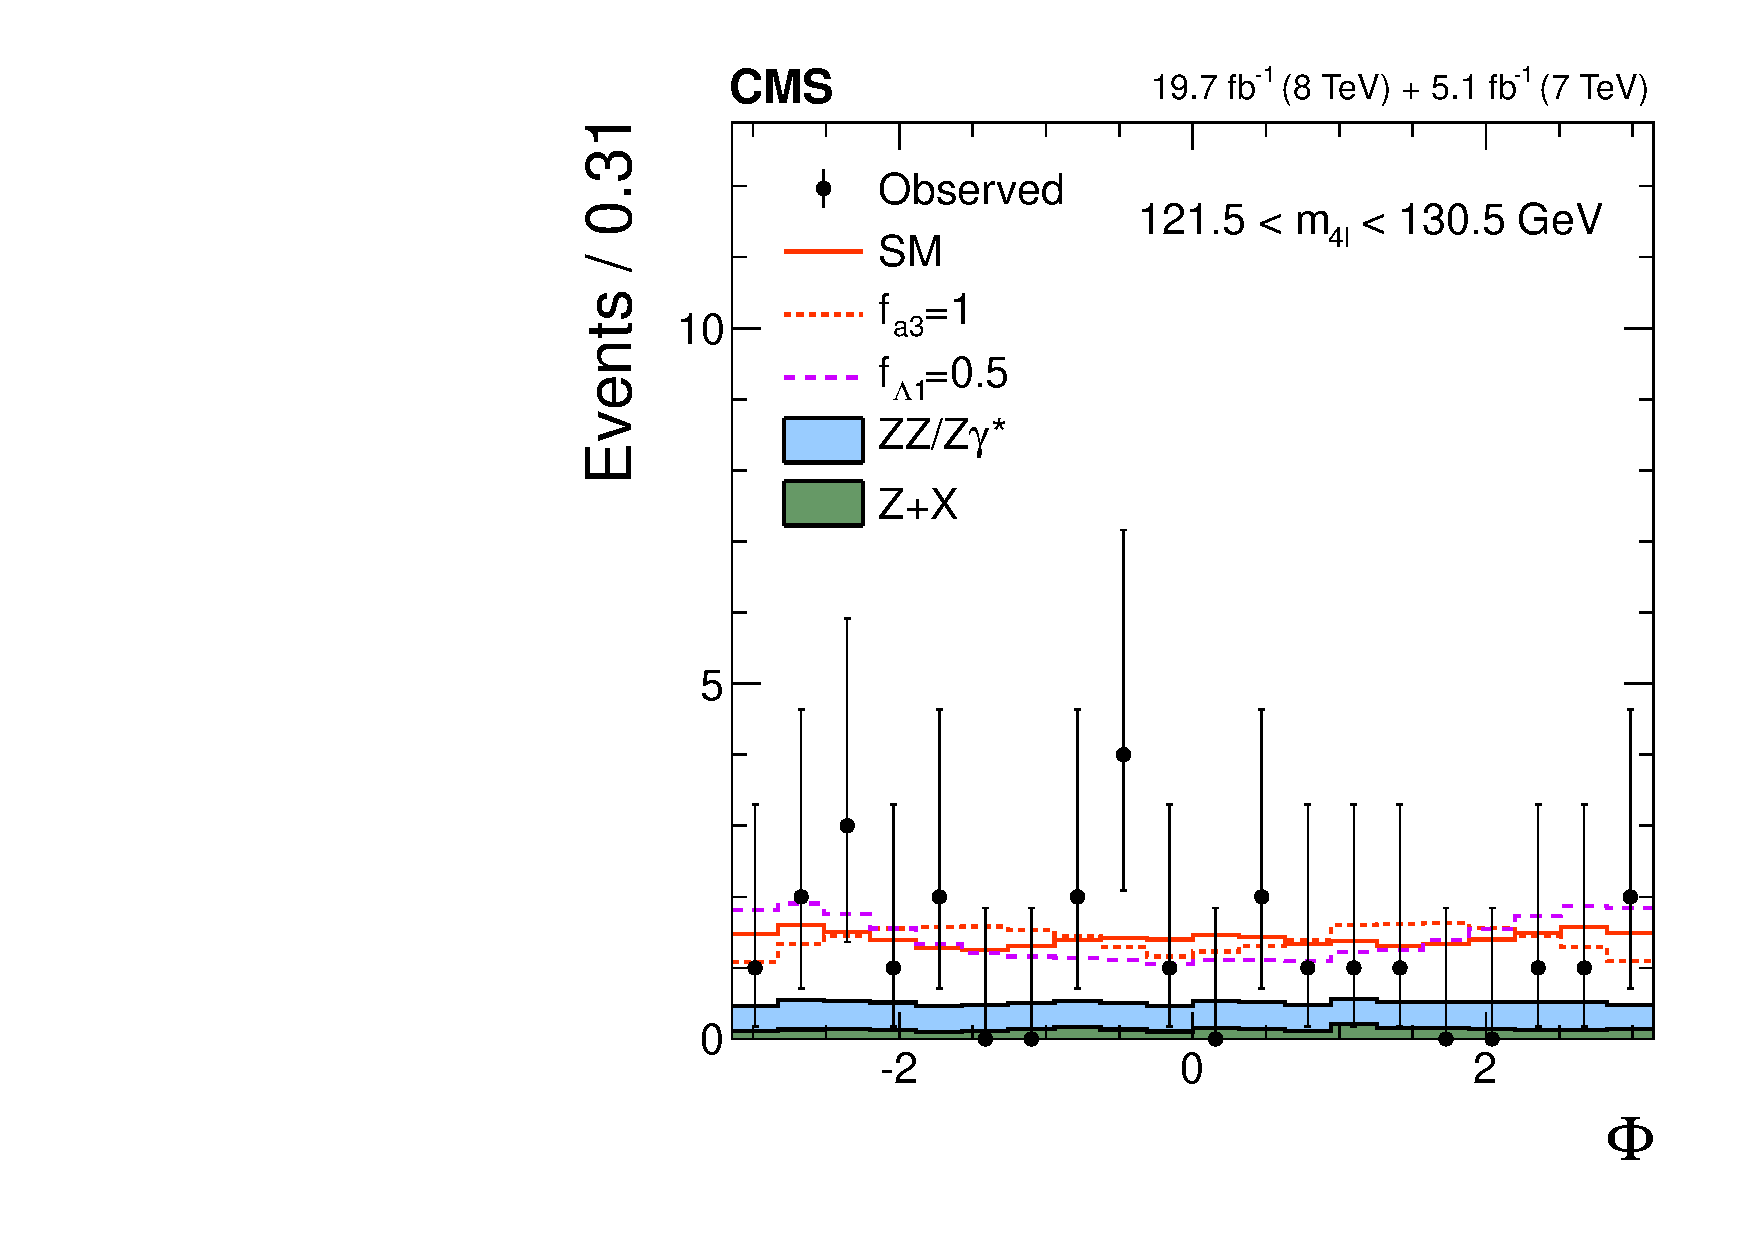
\includegraphics[width=0.32\textwidth]{HZZ4l_search/cCompare_DataMC_AllTeV_helphi_SignalEnriched.pdf}
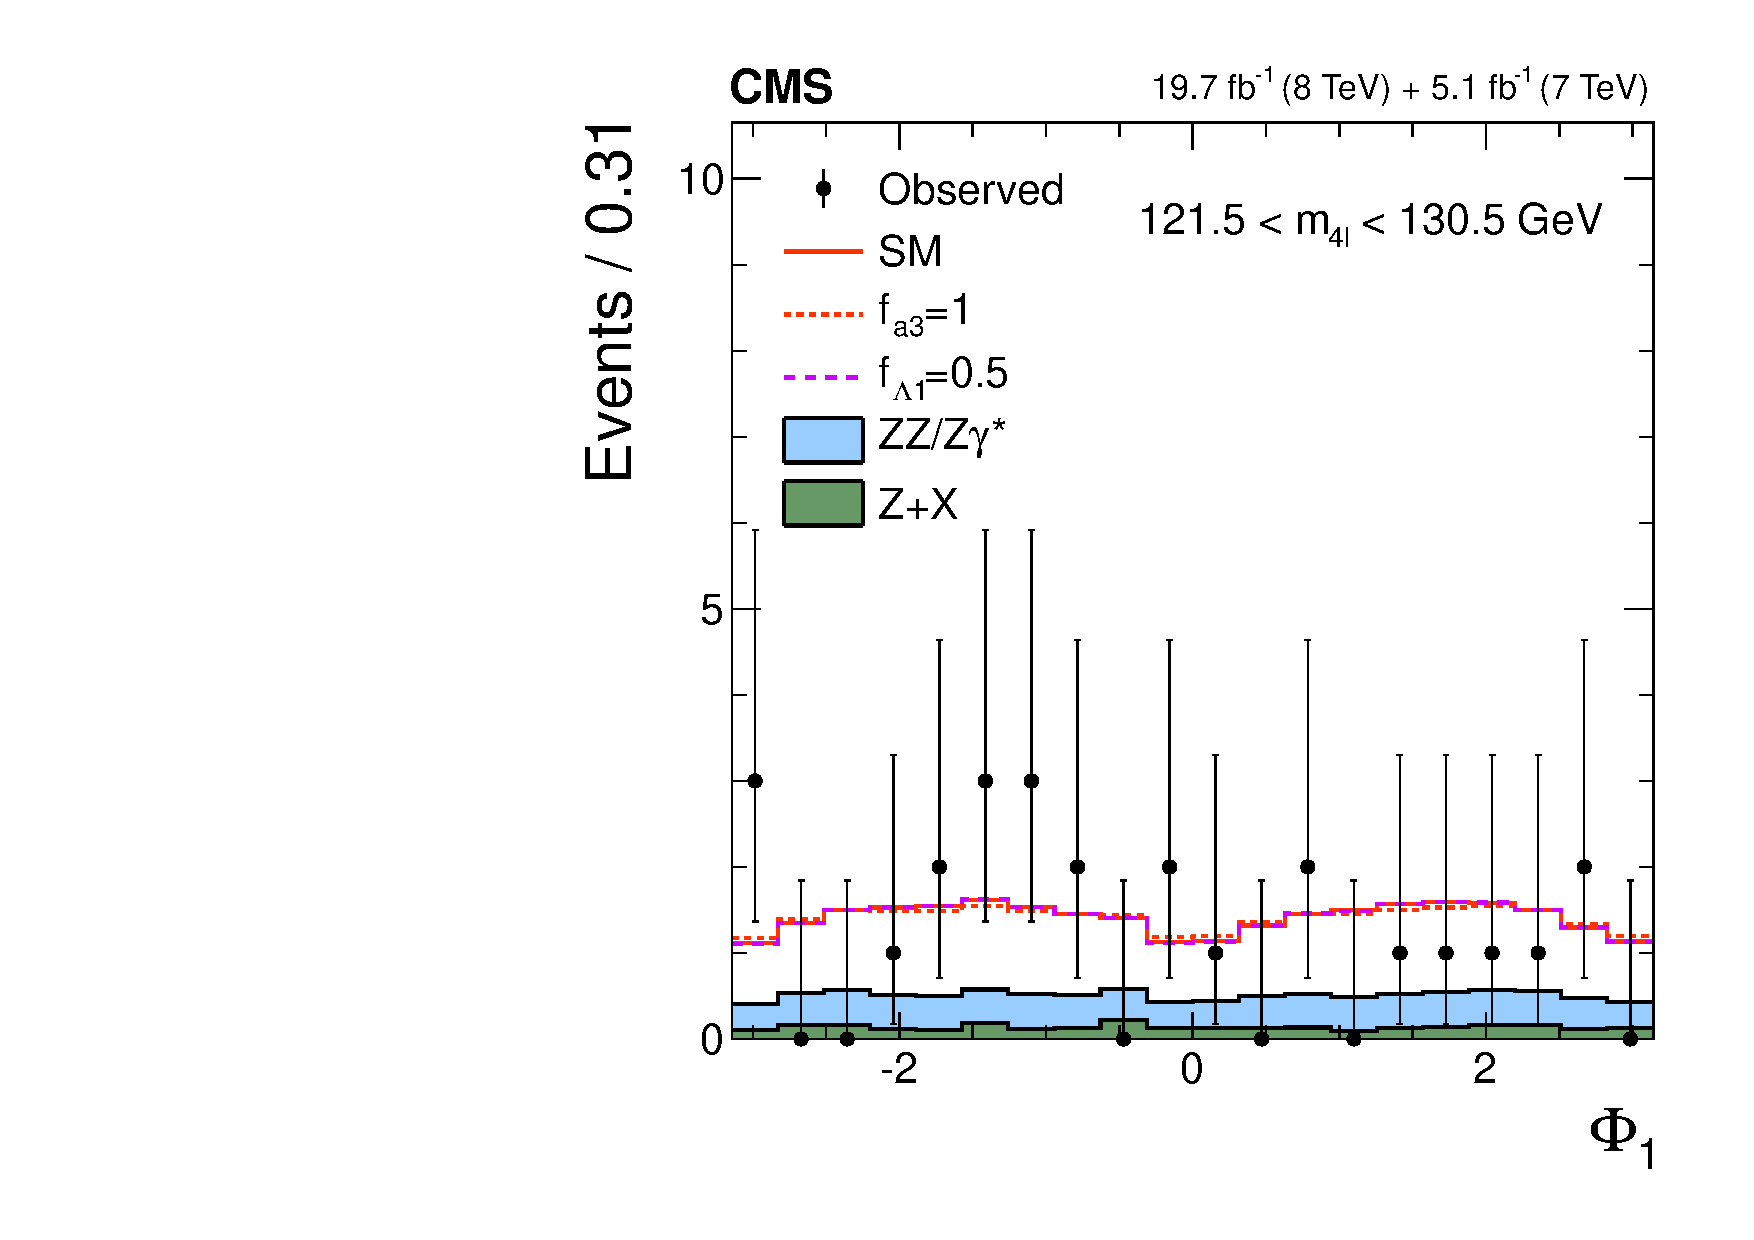
\includegraphics[width=0.32\textwidth]{HZZ4l_search/cCompare_DataMC_AllTeV_phistarZ1_SignalEnriched.pdf}
\caption[ Distributions of the eight kinematic observables used in the $H \to ZZ \to 4\ell$ analysis:
$m_{Z_1}$, $m_{Z_2}$, $\cos\theta^*$, $\cos\theta_{1}$, $\cos\theta_{2}$, $\Phi$, and $\Phi_{1}$.
The observed data (points with error bars), the expectations for the SM background (shaded areas),
the SM Higgs boson signal (open areas under the solid histogram),
and the alternative spin-zero resonances (open areas under the dashed histograms) are shown,
as indicated in the legend. The mass of the resonance is taken to be $\unit{125.6}{\GeV}$ and the SM cross section is used. All distributions, with the exception of $m_{4\ell}$, are presented with the requirement
$121.5 < m_{4\ell} < \unit{130.5}{\GeV}$.]{ Distributions of the eight kinematic observables used in the $H \to ZZ \to 4\ell$ analysis: $m_{Z_1}$, $m_{Z_2}$, $\cos\theta^*$, $\cos\theta_{1}$, $\cos\theta_{2}$, $\Phi$, and
$\Phi_{1}$.
The observed data (points with error bars), the expectations for the SM background (shaded areas),
the SM Higgs boson signal (open areas under the solid histogram),
and the alternative spin-zero resonances (open areas under the dashed histograms) are shown,
as indicated in the legend.
The mass of the resonance is taken to be $\unit{125.6}{\GeV}$ and the SM cross section is used.
All distributions, with the exception of $m_{4\ell}$, are presented with the requirement
$121.5 < m_{4\ell} < \unit{130.5}{\GeV}$ \cite{Khachatryan:2014kca}.}
\label{fig:kinematics}
\end{figure}

To separate a SM signal $\left(J^{P} = 0^{+}\right)$ from background a kinematic discriminant $\left(\mathcal{D}^{\text{kin}}_{\text{bkg}}\right)$ is defined based on the event probabilities $\mathcal{P}\left(m_{Z_{1}}, m_{Z_{1}}, \vec{\Omega} | m_{4\ell}\right)$ of the background or signal probability distribution of angular and mass observables computed from the LO matrix element squared for signal or ZZ processes. This discriminant is defined as in equation \eqref{eq:kd-mela}, giving the added advantage that to first order acceptance and phase space factors will cancel in the ratio. Thus, one does not need to integrate the matrix elements over the full kinematic range but simply calculate the magnitude of the matrix element squared at the point in phase space where each event appears.

The expected $\mathcal{D}^{\text{kin}}_{\text{bkg}}$ shapes for signal and the $q\bar{q} \to ZZ$ and $gg \to ZZ$ backgrounds are taken from simulation of the three decay channels $4e$, $2e2\mu$, and $4\mu$ independently. Given the low statistics and unreliable simulation of the $Z + \text{jets}$ contribution is modeled by collision events in the control regions. The statistics are boosted by merging all decay channels and control regions together using the appropriate weight to map them to the signal region. 

\begin{equation}
  \label{eq:kd-mela}
  \mathcal{D}^{\text{kin}}_{\text{bkg}} = \frac{\mathcal{P}^\text{kin}_{0^+} }{\mathcal{P}^\text{kin}_{0^+} +\mathcal{P}^\text{kin}_\text{bkg} }=
  \left[1+\frac{\mathcal{P}^\text{kin}_\text{bkg}(m_{Z_1}, m_{Z_2}, \vec\Omega | m_{4\ell})}
    {\mathcal{P}^\text{kin}_{0^+} (m_{Z_1}, m_{Z_2}, \vec\Omega | m_{4\ell})}  \right]^{-1}. \\
\end{equation}

Because these discriminant values do not directly carry $m_{4\ell}$ discrimination power they are used as a second dimensions for discrimination between signal and background. The distributions of the $\mathcal{D}^{\text{kin}}_{\text{bkg}}$ versus $m_{4\ell}$ are shown for the selected events and compared to the SM background expectation in figure \ref{fig:KDvsM4lFullMass}. The distribution of events in the $\left(m_{4\ell}, \mathcal{D}^{\text{kin}}_{\text{bkg}}\right)$ plane agrees well with the SM background expectation in the high-mass range, figure \ref{fig:KDvsM4lFullMass}~(right), while discrepancies in the two-dimensional plane are observed in the low-mass range $110<m_{4\ell}<\unit{180}{\GeV}$, figure~\ref{fig:KDvsM4lFullMass}~(left), indicative of the presence of a signal.


\begin{figure}
  \begin{center}
    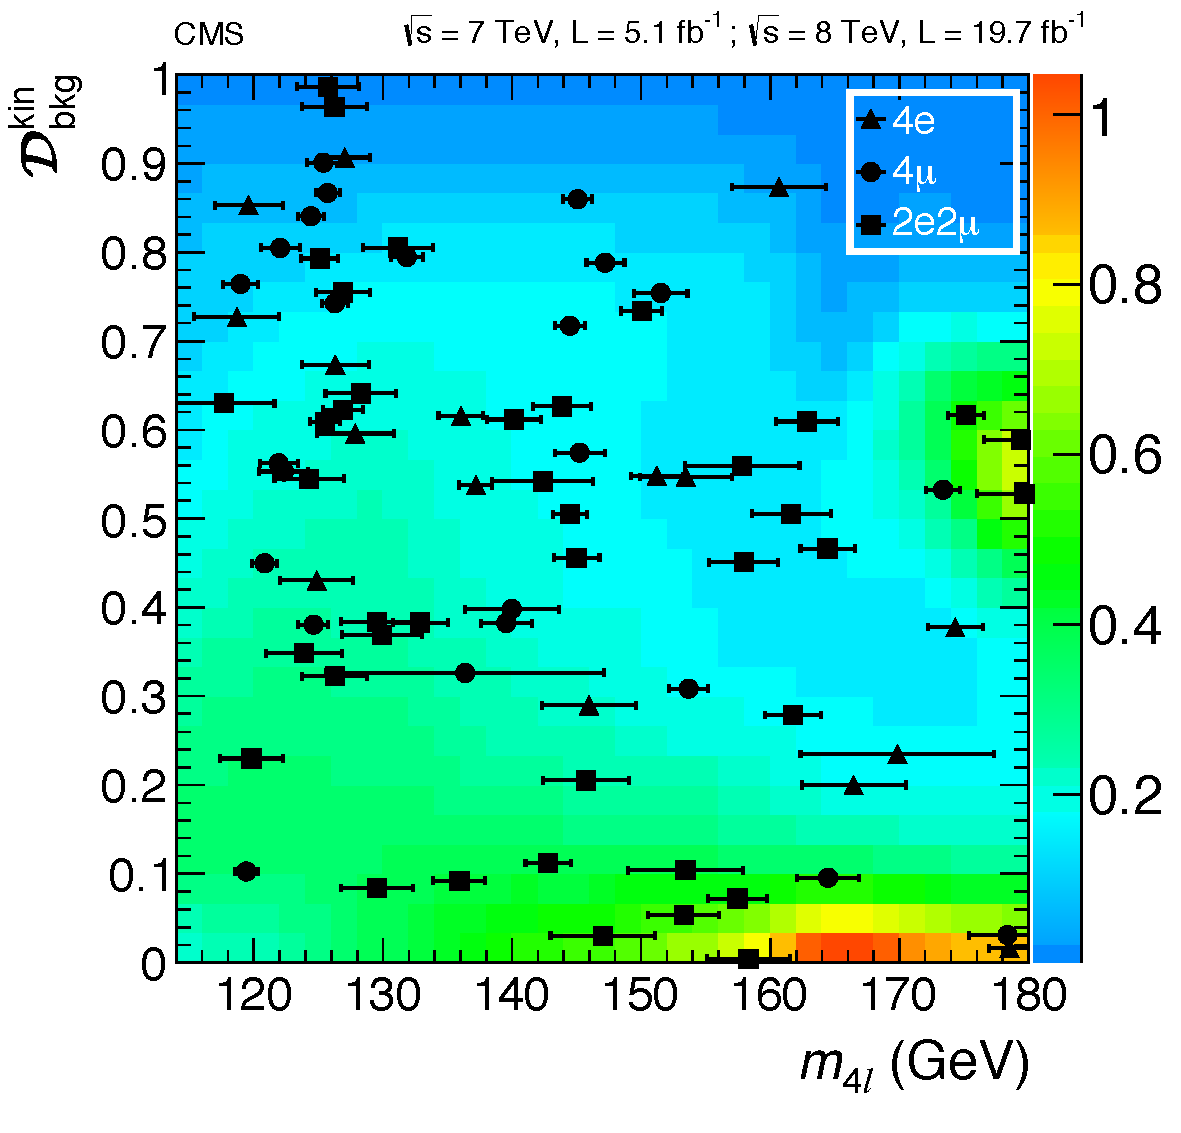
\includegraphics[width=0.45\textwidth]{HZZ4l_search/KD_vs_m4l_lowMass_Back.pdf}
    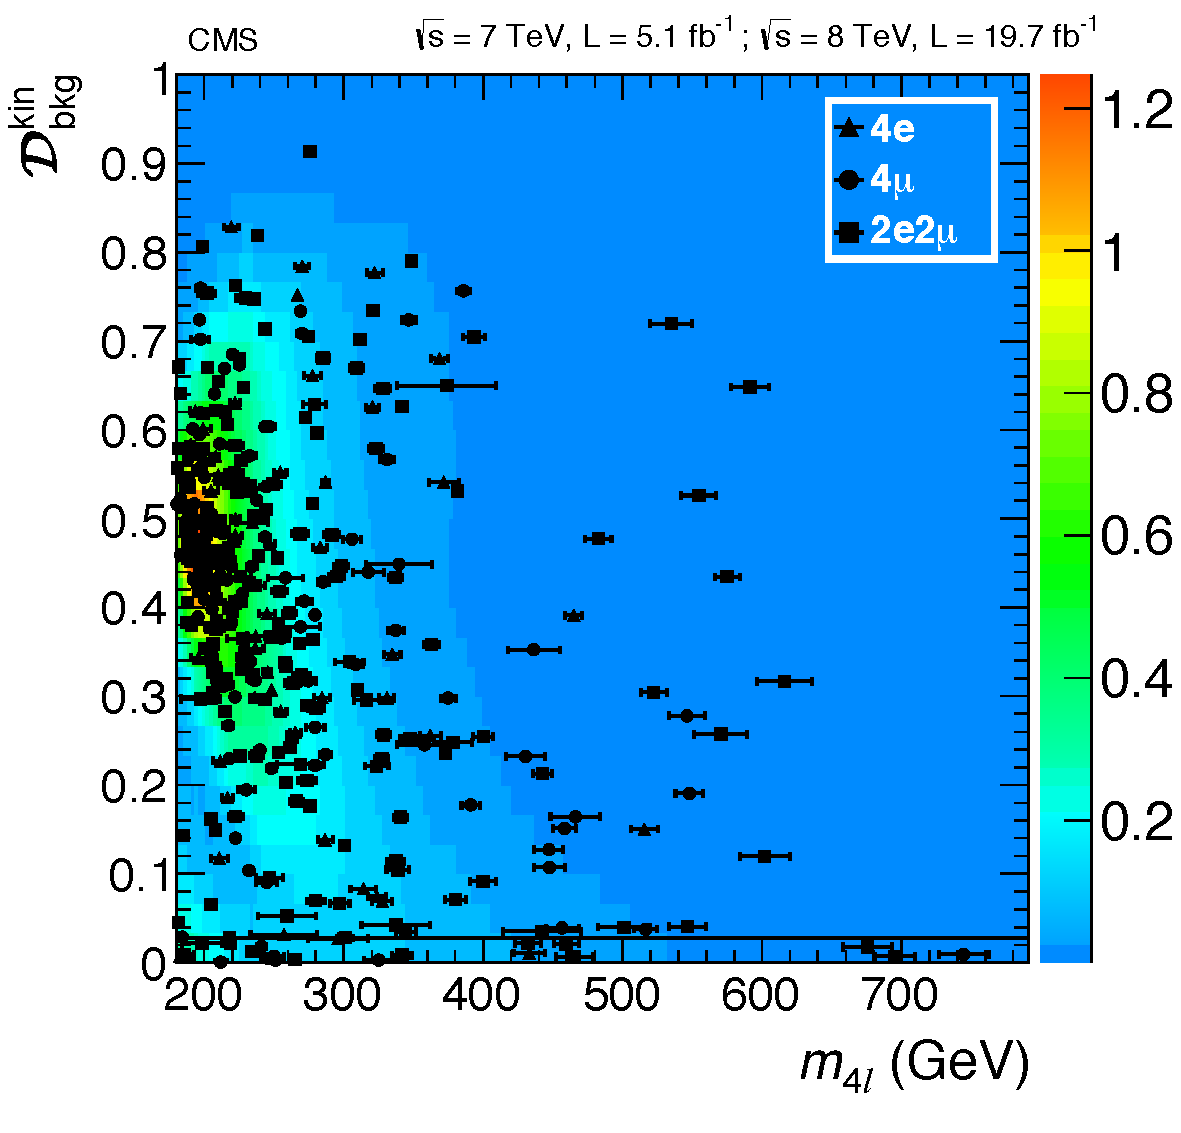
\includegraphics[width=0.45\textwidth]{HZZ4l_search/KD_vs_m4l_highMass_Back.pdf}
    \caption[Distribution of the kinematic discriminant $\mathcal{D}^{\text{kin}}_{\text{bkg}}$ versus
      the four-lepton reconstructed mass $m_{4\ell}$ in the (left)
      low-mass and (right) high-mass regions.  The color scale represents
      the expected relative density in linear scale (in arbitrary
      units) of background events.  The points show the data and the
      measured per-event invariant mass uncertainties as horizontal
      bars. One $2e2\mu$ event with $m_{4\ell}\approx \unit{220}{\GeV}$ and
      small $\mathcal{D}^{\text{kin}}_{\text{bkg}}$ has a huge mass uncertainty, and it is displayed as the
      horizontal line. No events are observed for $m_{4\ell}>\unit{800}{\GeV}$.]{Distribution of the kinematic discriminant $\mathcal{D}^{\text{kin}}_{\text{bkg}}$ versus
      the four-lepton reconstructed mass $m_{4\ell}$ in the (left)
      low-mass and (right) high-mass regions.  The color scale represents
      the expected relative density in linear scale (in arbitrary
      units) of background events.  The points show the data and the
      measured per-event invariant mass uncertainties as horizontal
      bars. One $2e2\mu$ event with $m_{4\ell}\approx \unit{220}{\GeV}$ and
      small $\mathcal{D}^{\text{kin}}_{\text{bkg}}$ has a huge mass uncertainty, and it is displayed as the
      horizontal line. No events are observed for $m_{4\ell}>\unit{800}{\GeV}$ \cite{Chatrchyan:2013mxa}.
      \label{fig:KDvsM4lFullMass}}
  \end{center}
\end{figure}

Figure~\ref{fig:KDLow}~(left) shows the same data points as in figure ~\ref{fig:KDvsM4lFullMass}~(left), but compared with the expected distribution from SM backgrounds plus the contribution of a Higgs boson with $m_H = \unit{126}{\GeV}$. A signal-like clustering of events is apparent at high values of $\mathcal{D}^{\text{kin}}_{\text{bkg}}$ and for $m_{4\ell} \approx \unit{126}{\GeV}$.  Figure~\ref{fig:KDLow}~(right) shows the distribution of the kinematic discriminant $\mathcal{D}^{\text{kin}}_{\text{bkg}}$ in the mass region $121.5 < m_{4\ell} < \unit{130.5}{\GeV}$.

\begin{figure}
  \begin{center}
    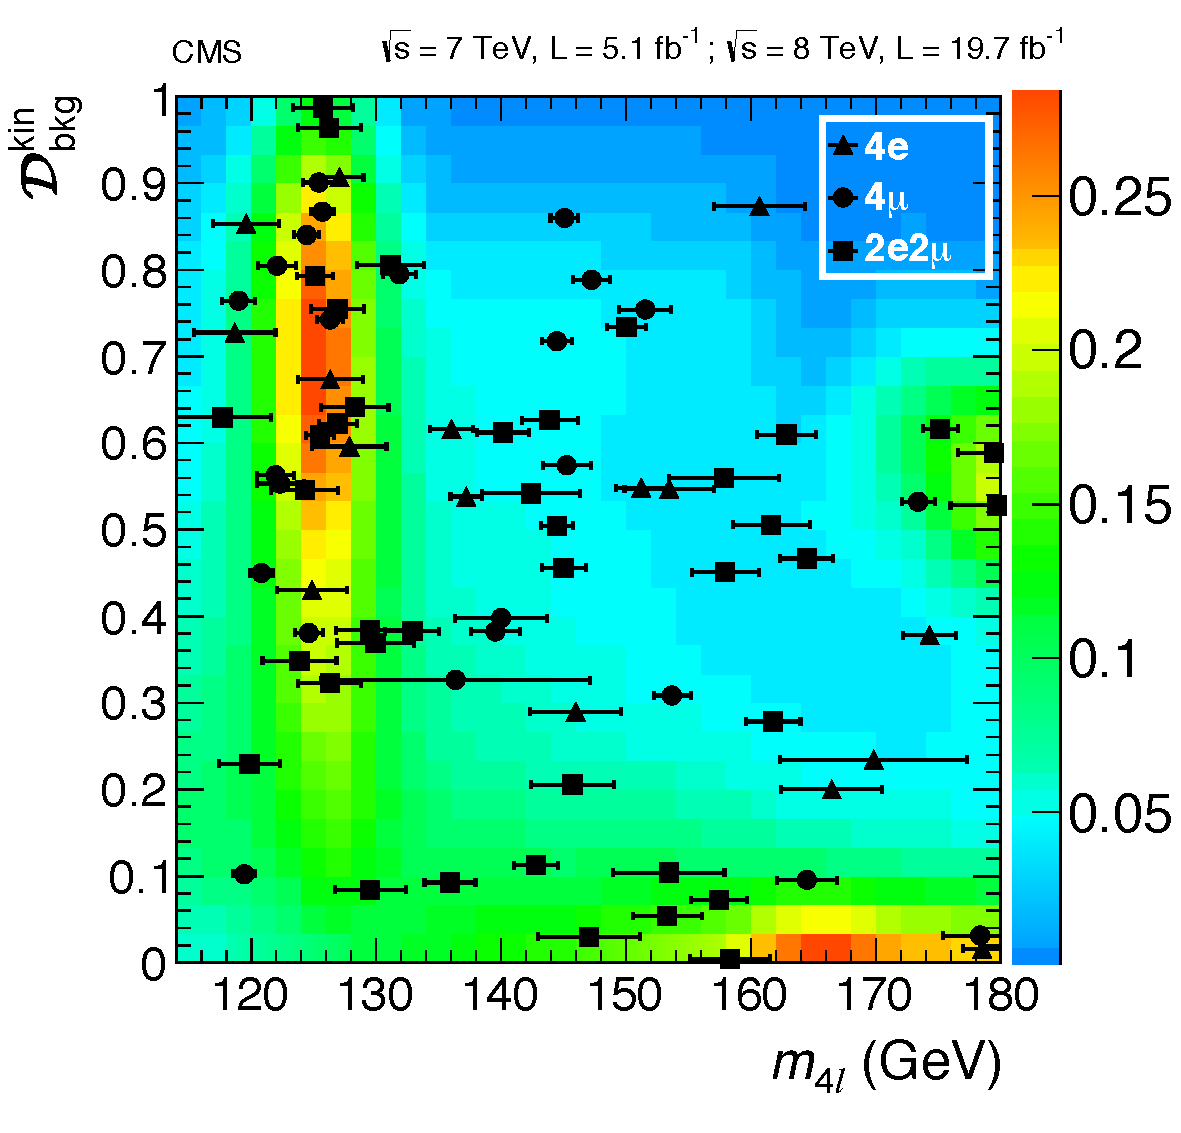
\includegraphics[width=0.45\textwidth]{HZZ4l_search/KD_vs_m4l_lowMass_Signal.pdf}
    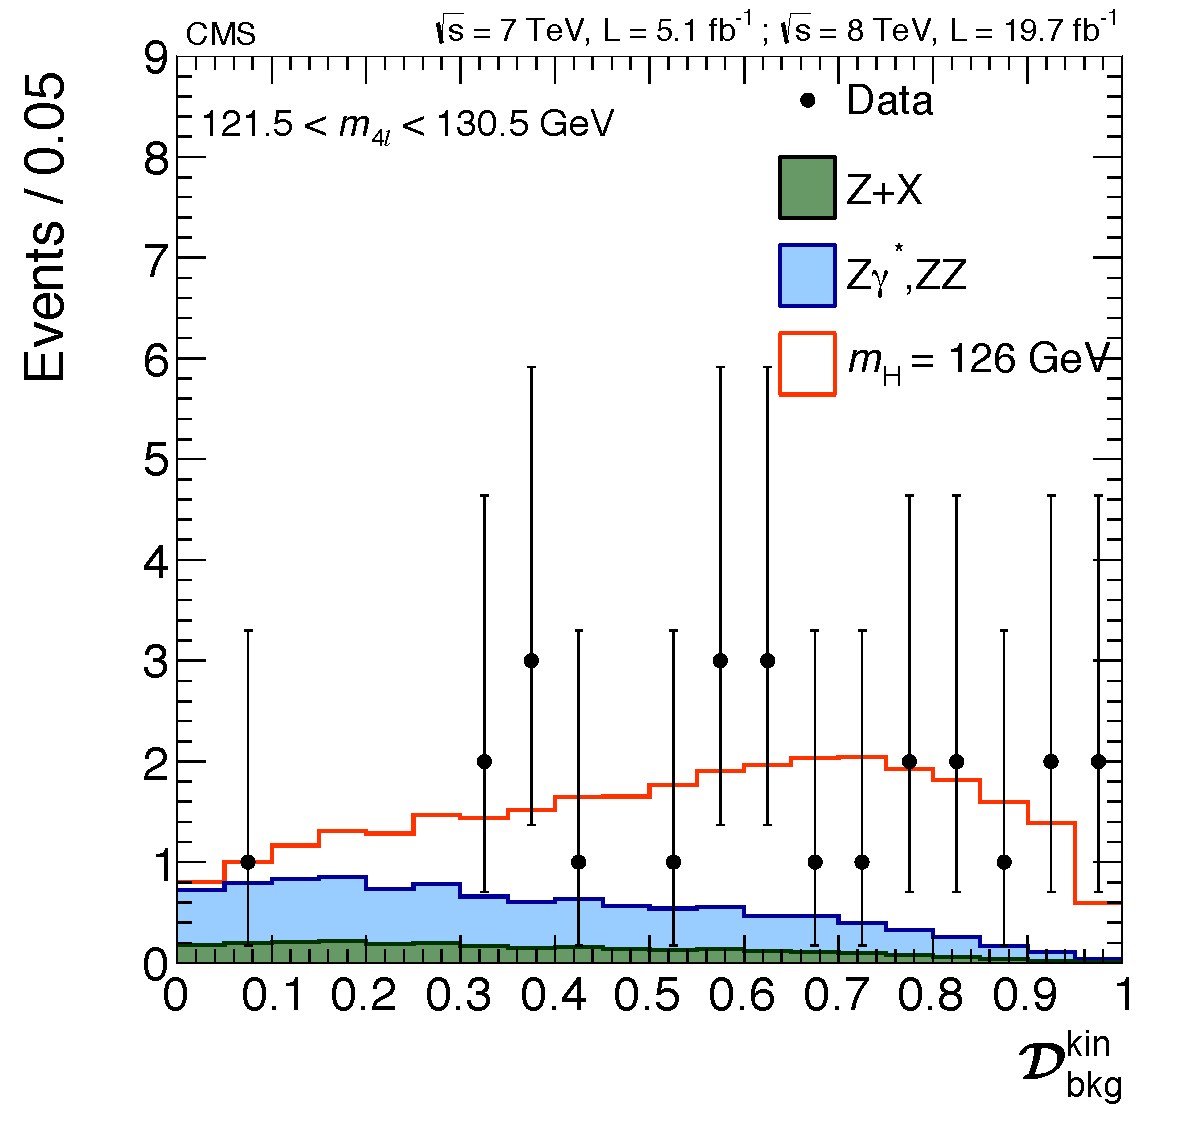
\includegraphics[width=0.45\textwidth]{HZZ4l_search/KDPeak.pdf}
        \caption[(left) Distribution of $\mathcal{D}^{\text{kin}}_{\text{bkg}}$ versus $m_{4\ell}$ in
      the low-mass range with colors shown for the expected relative
      density in linear scale (in arbitrary units) of background plus
      the Higgs boson signal for $m_H=\unit{126}{\GeV}$. The points show the data,
      and horizontal bars represent the measured mass
      uncertainties. (right) Distribution of the kinematic
      discriminant $\mathcal{D}^{\text{kin}}_{\text{bkg}}$ for events in the mass region $121.5 <
      m_{4\ell} < \unit{130.5}{\GeV}$.  Points with error bars represent the
      data, shaded histograms represent the backgrounds, and the
      unshaded histogram the signal expectation.  Signal and
      background histograms are
      stacked.]{(left) Distribution of $\mathcal{D}^{\text{kin}}_{\text{bkg}}$ versus $m_{4\ell}$ in
      the low-mass range with colors shown for the expected relative
      density in linear scale (in arbitrary units) of background plus
      the Higgs boson signal for $m_H=\unit{126}{\GeV}$. The points show the data,
      and horizontal bars represent the measured mass
      uncertainties. (right) Distribution of the kinematic
      discriminant $\mathcal{D}^{\text{kin}}_{\text{bkg}}$ for events in the mass region $121.5 <
      m_{4\ell} < \unit{130.5}{\GeV}$.  Points with error bars represent the
      data, shaded histograms represent the backgrounds, and the
      unshaded histogram the signal expectation.  Signal and
      background histograms are
      stacked \cite{Chatrchyan:2013mxa}.  \label{fig:KDLow}} \end{center}
\end{figure}

\subsection{$p_{T}^{4\ell}$ and Jet Kinematic Discriminant}
\label{sec:pT_Djet}

While in the dominant gluon fusion mechanism the Higgs boson is
the most likely way to produce a Higgs boson at the LHC,  the cross
section for VBF production is only about 1 order of magnitude smaller than
that for the gluon fusion process.  In the vector-boson scattering
process, the two initial-state quarks deviate at a polar angle large
enough such that as final-state quarks they create measurable
additional jets in the event.  These two jets, being remnants of the
incoming proton beams, have typically a large separation in $\eta$ and
high momentum.  These characteristics are used to distinguish gluon
fusion from VBF Higgs boson production in the analysis. Jets in the
final state also come from $t\bar{t}H$ and $VH$ production, where
the $V$ decays hadronically.

In the 0/1-jet category, the transverse
momentum of the four-lepton system ($p_{T}^{4\ell}$) is used to distinguish VBF
production and associated production with a weak boson, $VH$, from
gluon fusion, discrimination power seen in figure \ref{fig:vbfVars} (top right). 
In the dijet category, a linear discriminant ($\mathcal{D}_{\text{jet}}$) is
formed combining two VBF-sensitive variables, the absolute difference
in pseudorapidity ($\abs{\Delta\eta_{jj}}$) and the invariant mass of the two leading jets
($m_{jj}$). The discriminant maximizes the separation between
vector-boson and gluon fusion processes. In the 0/1-jet (dijet)
category, about 5\% (20\%) of the signal events are expected to come
from the VBF production mechanism, as estimated from simulation. Simulations of these distributions are shown in figure \ref{fig:vbfVars}.

\begin{figure}
\begin{center}
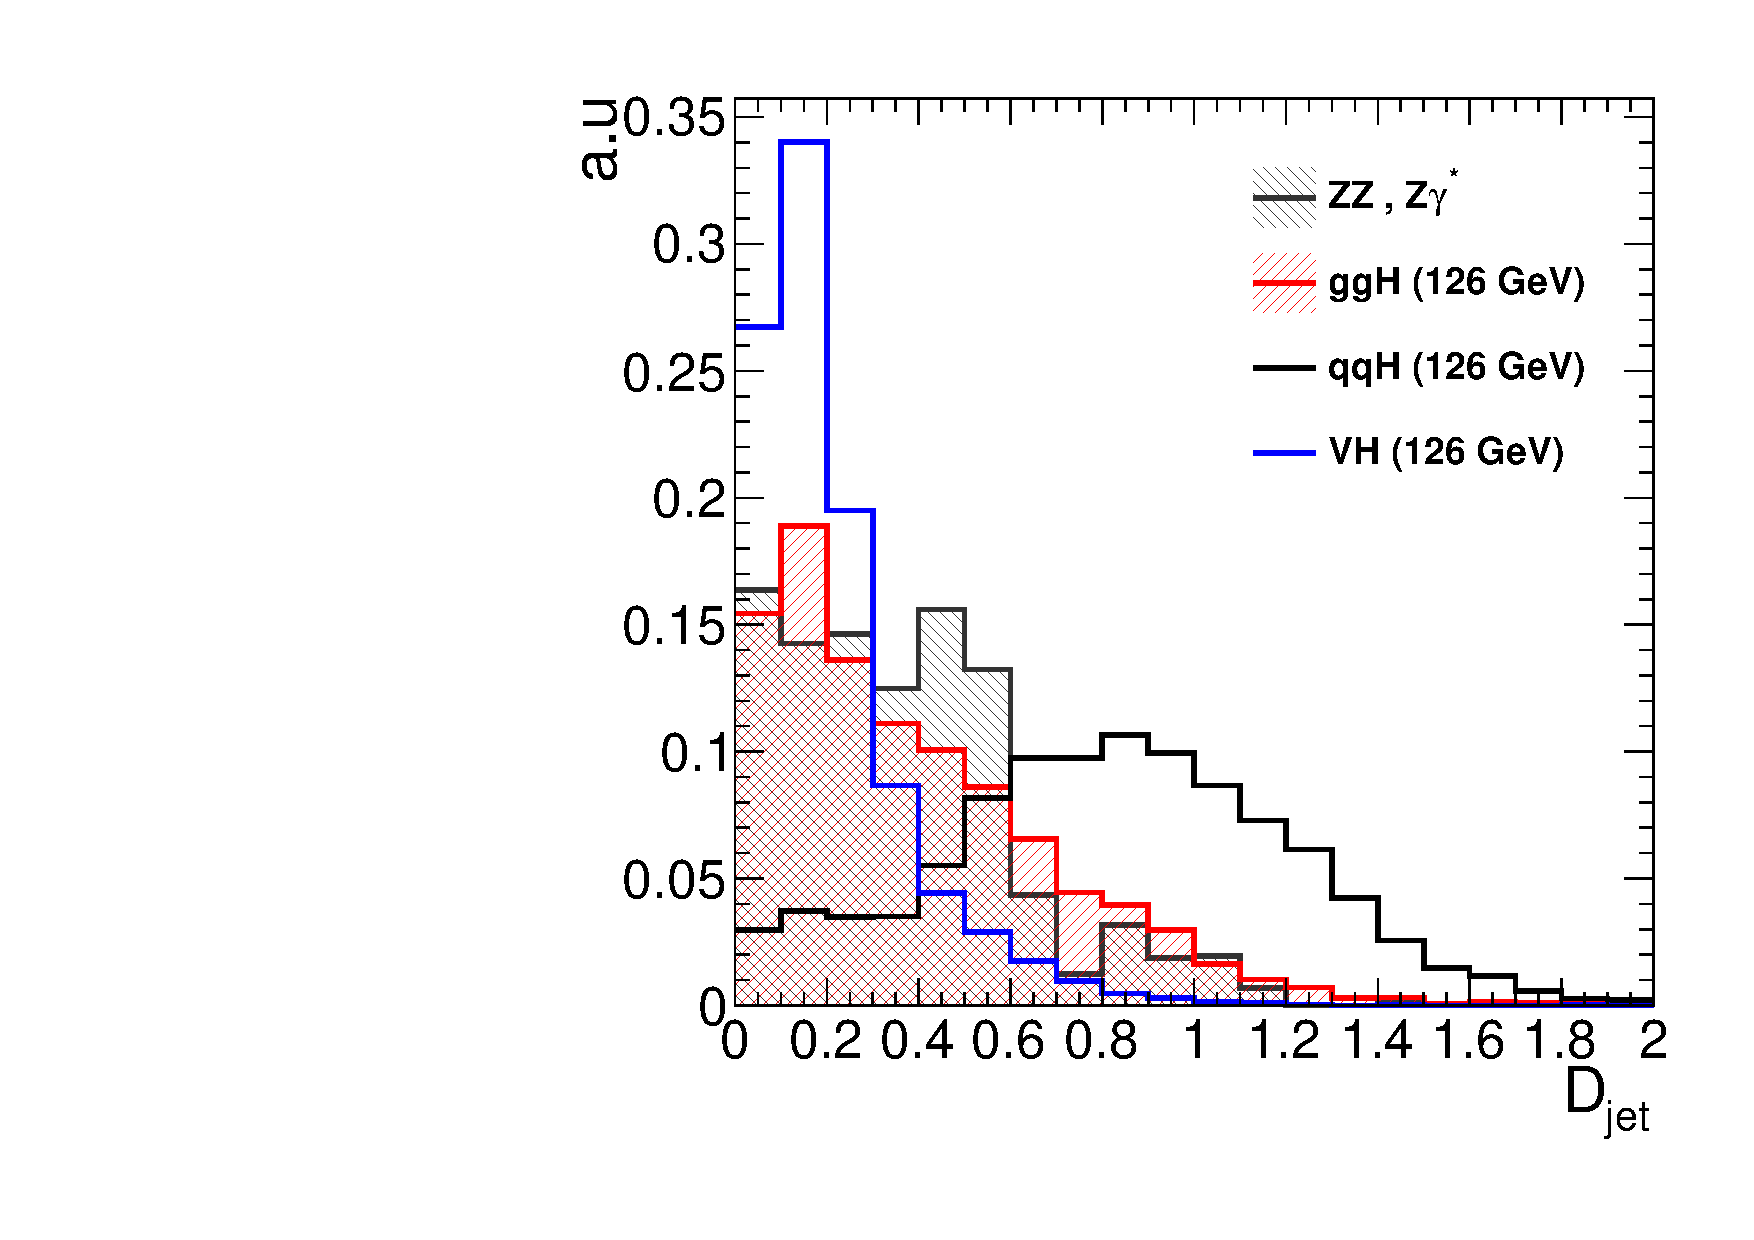
\includegraphics[width=0.4\textwidth]{HZZ4l_search/djet_shape.pdf}
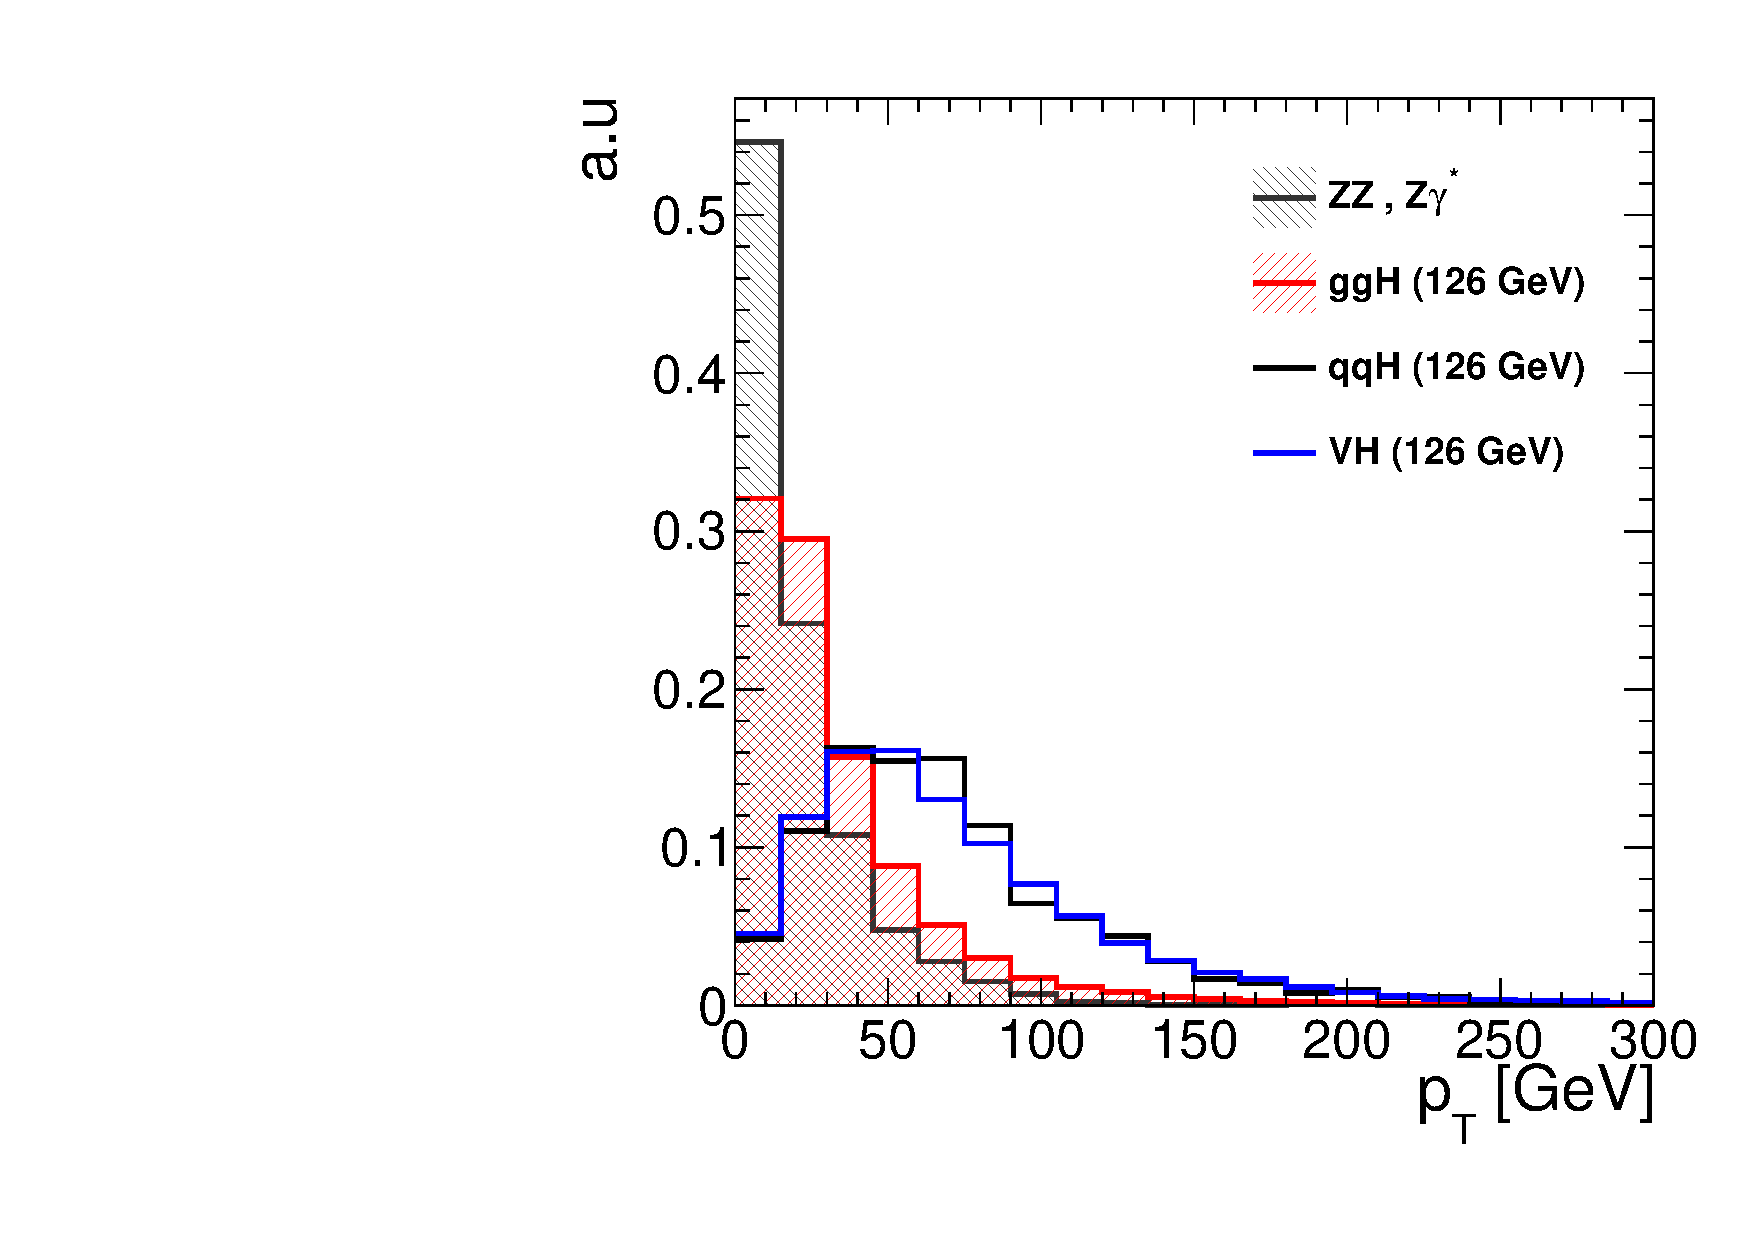
\includegraphics[width=0.4\textwidth]{HZZ4l_search/pt_shape.pdf} \\
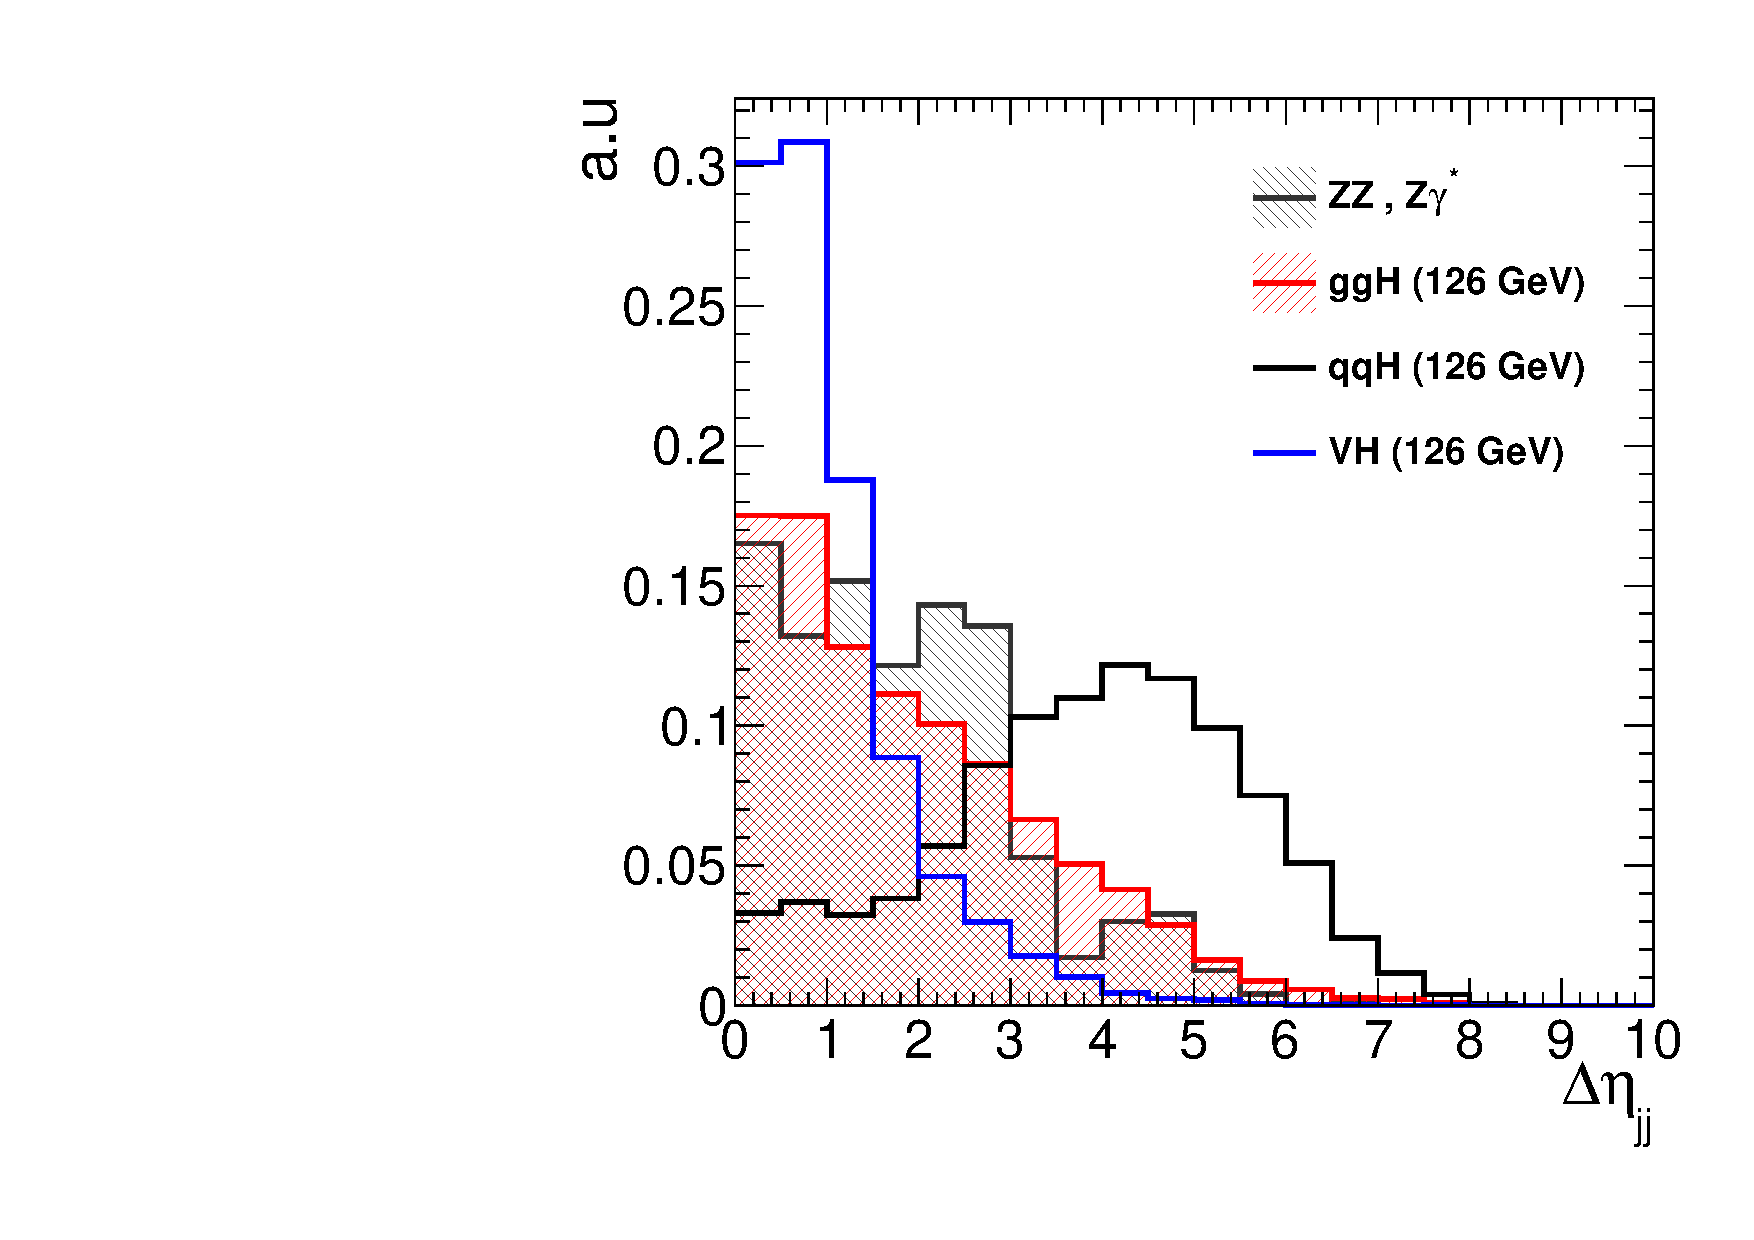
\includegraphics[width=0.4\textwidth]{HZZ4l_search/deta_shape.pdf}
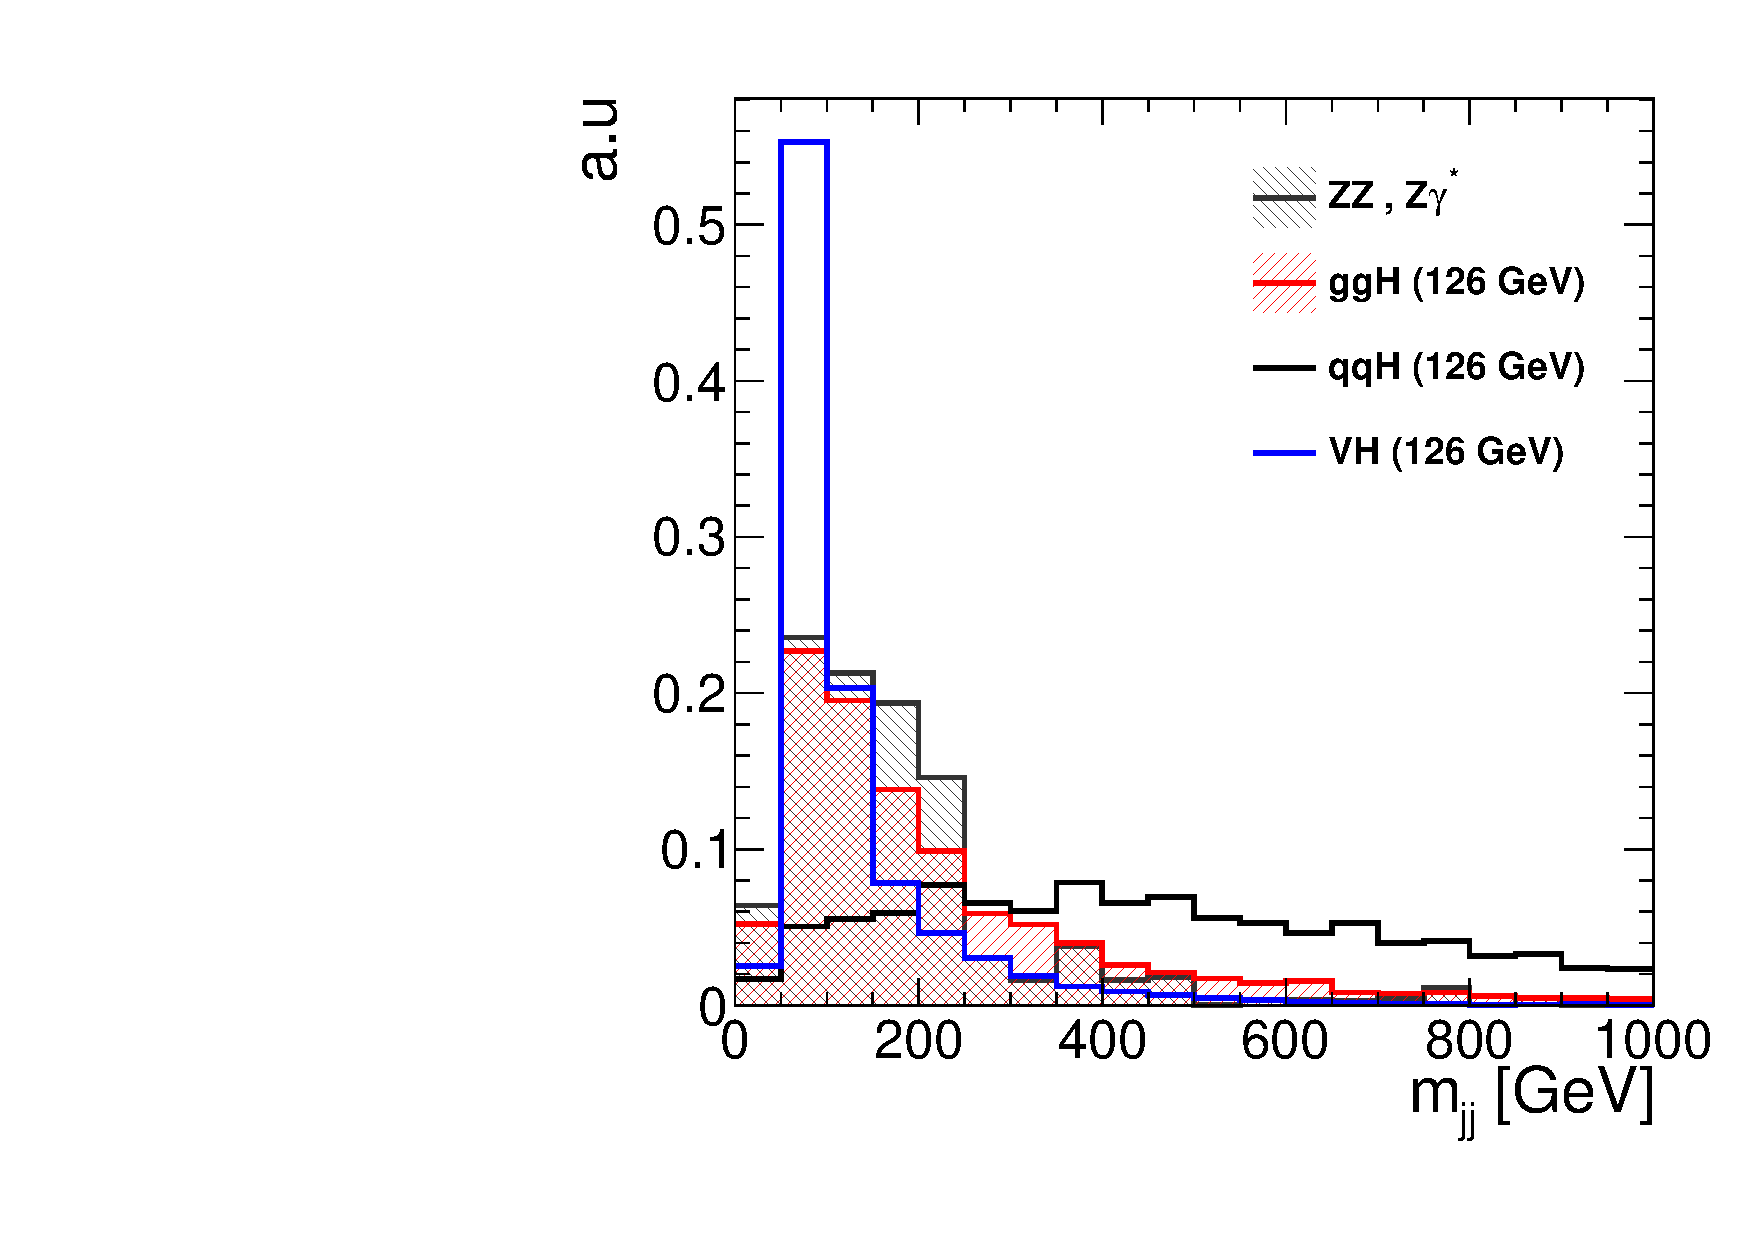
\includegraphics[width=0.4\textwidth]{HZZ4l_search/mjj_shape.pdf} \\
\caption[Main observables discriminating production mechanisms in 0/1 jet and Dijet categories in arbitrary units. $q\bar{q}H$ is used in these figures for VBF production. (top left) $\mathcal{D}_{\text{jet}}$ Discriminant combining VBF discrimination variables. (top right) $p_T$ of the four-lepton system. (bottom left) $\Delta\eta$ of the two leading jets. (bottom right) Invariant mass of the two jets.]{Main observables discriminating production mechanisms in 0/1 jet and Dijet categories in arbitrary units. $q\bar{q}H$ is used in these figures for VBF production. (top left) $\mathcal{D}_{\text{jet}}$ Discriminant combining VBF discrimination variables. (top right) $p_T$ of the four-lepton system. (bottom left) $\Delta\eta$ of the two leading jets. (bottom right) Invariant mass of the two jets.}   
\label{fig:vbfVars}
\end{center}
\end{figure}


For the final analysis, the distribution of the transverse momentum of the $4\ell$ system in
 the 0/1-jet category and its joint distribution with $m_{4\ell}$ are
 shown in figure \ref{fig:DpTLow}. The $p_{T}$ spectrum shows good
 agreement with a SM Higgs boson hypothesis with $m_{H} = \unit{126}{\GeV}$ in the
 0/1-jet category with few events having $p_{T}>\unit{60}{\GeV}$, where VBF and
 $VH$ production are relatively more relevant.
 
 \begin{figure}
  \begin{center}
    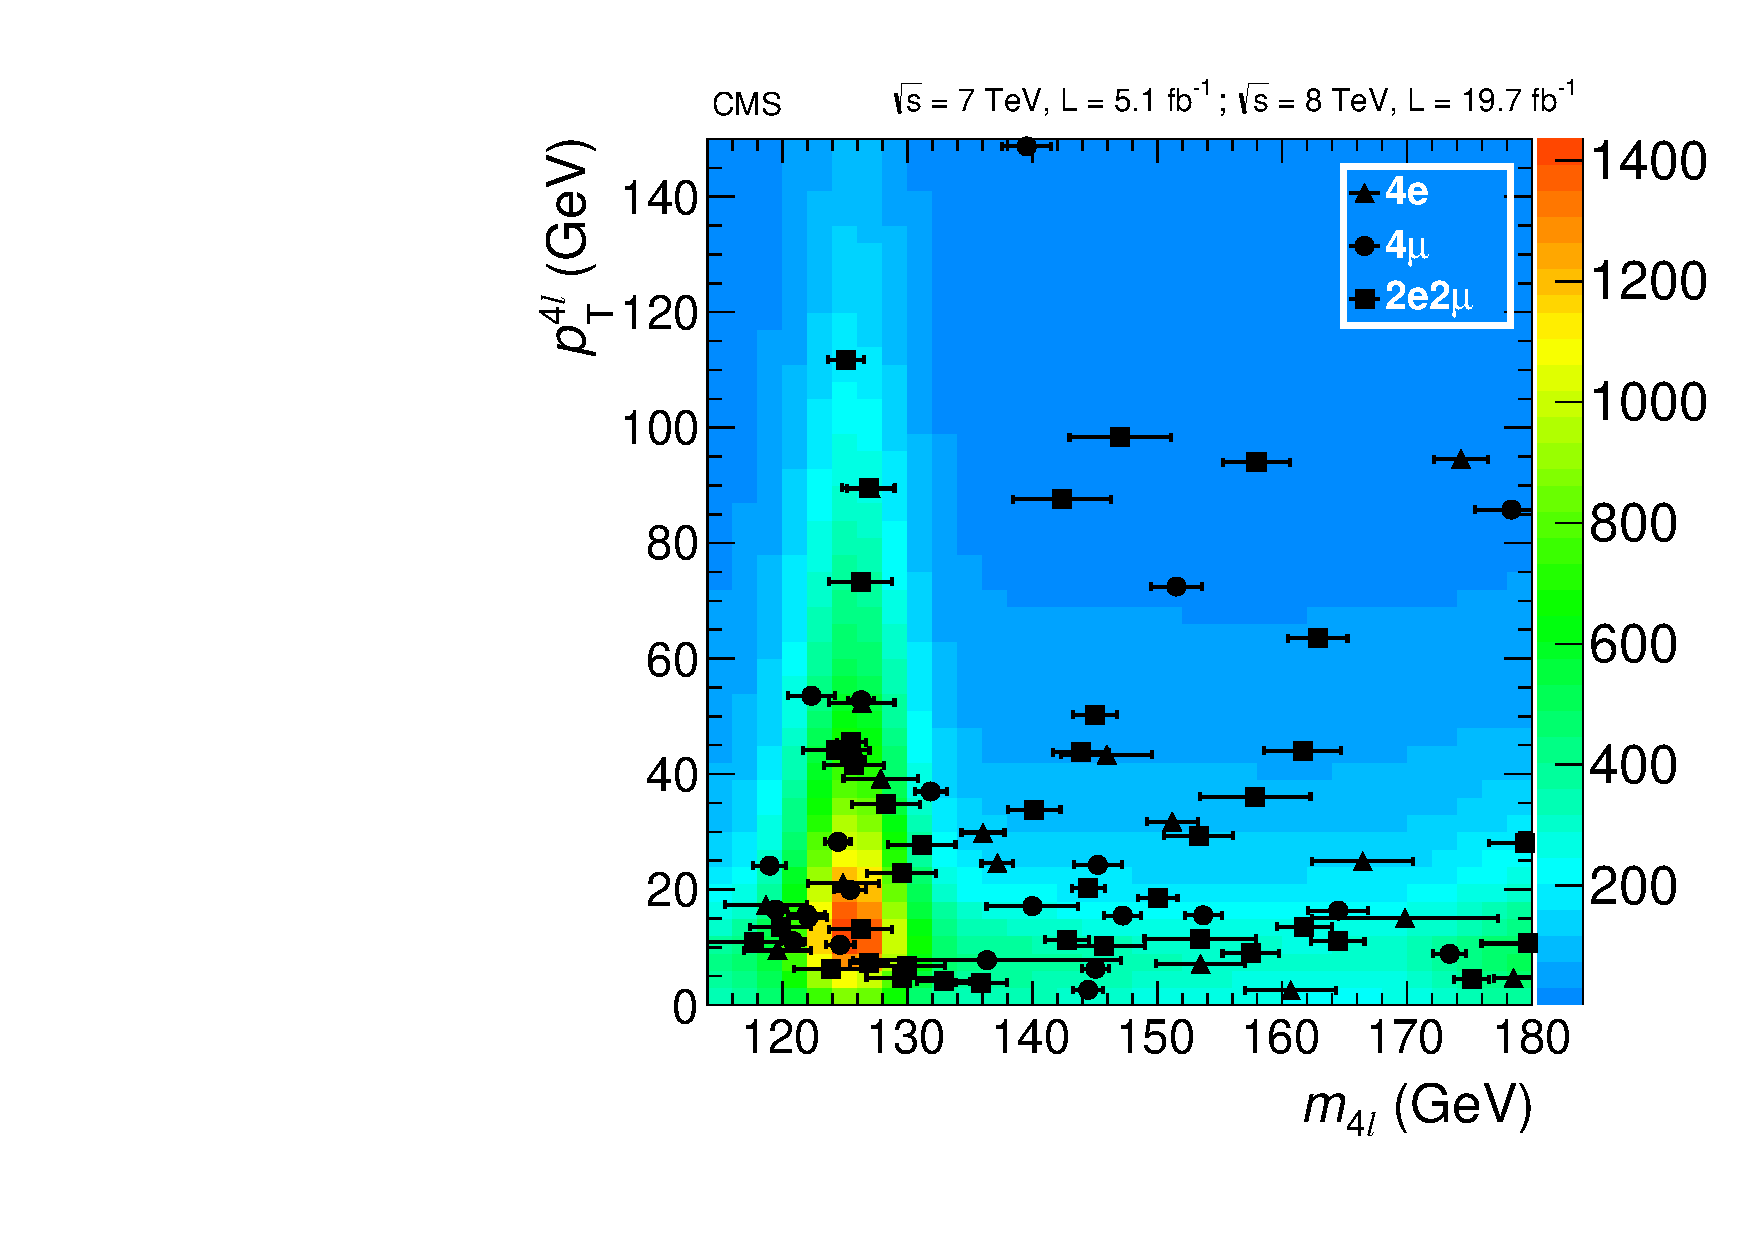
\includegraphics[width=0.45\textwidth]{HZZ4l_search/M4l_vs_pT_all.pdf}
    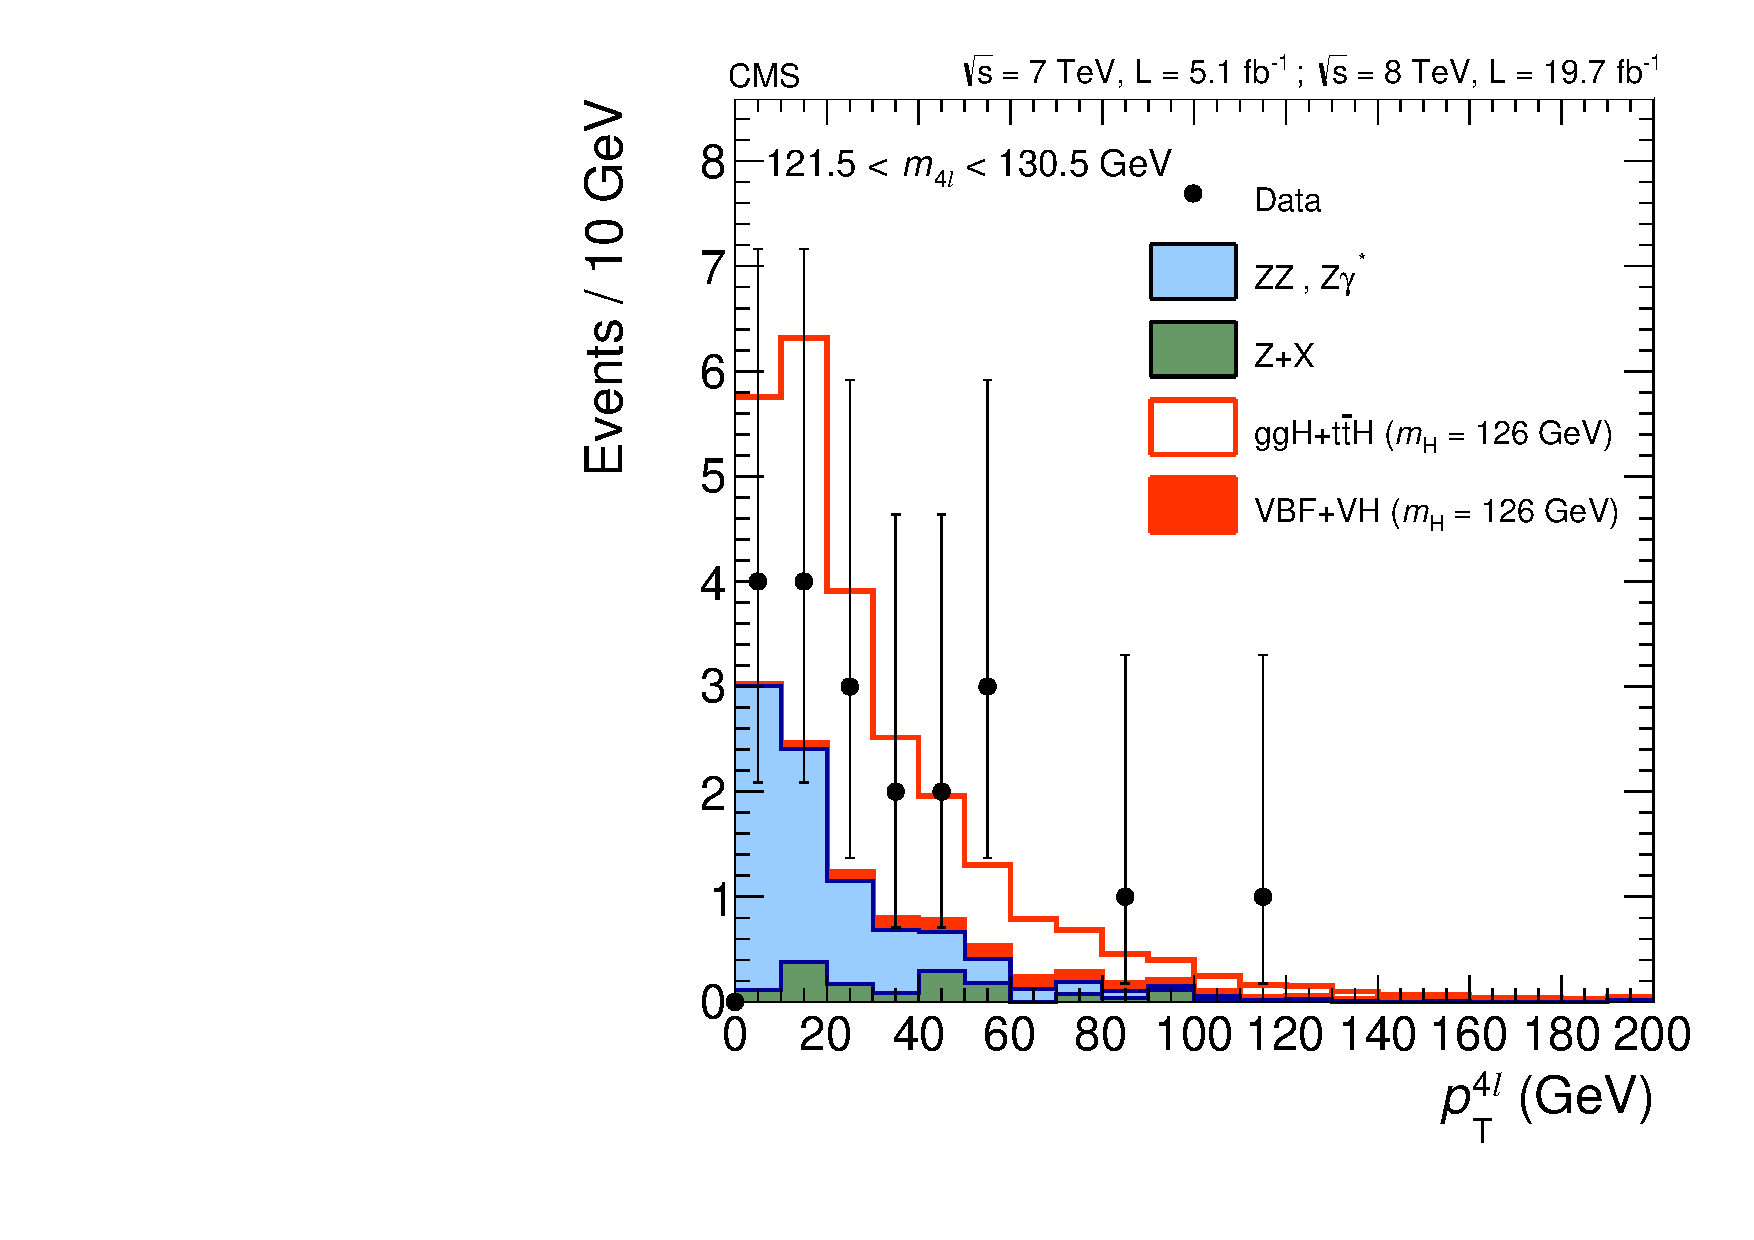
\includegraphics[width=0.45\textwidth]{HZZ4l_search/PT01JetPeak.pdf}
    \caption[(left) Distribution of $p_{T}^{4\ell}$ versus $m_{4\ell}$ in the
      low-mass-range 0/1-jet category with colors shown for the
      expected relative density in linear scale (in arbitrary units)
      of background plus the Higgs boson signal for $m_H=\unit{126}{\GeV}$. No
      events are observed for $p_{T}^{4\ell}>150$\GeV. The points show the data,
      and horizontal bars represent the measured mass
      uncertainties. (right) Distribution of $p_{T}^{4\ell}$ in the 0/1-jet
      category for events in the mass region $121.5 < m_{4\ell} <
      \unit{130.5}{\GeV}$.  Points with error bars represent the data, shaded
      histograms represent the backgrounds, and the red histograms represent the
      signal expectation, broken down by production mechanism. Signal
      and background histograms are stacked.]{(left) Distribution of $p_{T}^{4\ell}$ versus $m_{4\ell}$ in the
      low-mass-range 0/1-jet category with colors shown for the
      expected relative density in linear scale (in arbitrary units)
      of background plus the Higgs boson signal for $m_H=\unit{126}{\GeV}$. No
      events are observed for $p_{T}^{4\ell}>150$\GeV. The points show the data,
      and horizontal bars represent the measured mass
      uncertainties. (right) Distribution of $p_{T}^{4\ell}$ in the 0/1-jet
      category for events in the mass region $121.5 < m_{4\ell} <
      \unit{130.5}{\GeV}$.  Points with error bars represent the data, shaded
      histograms represent the backgrounds, and the red histograms represent the
      signal expectation, broken down by production mechanism. Signal
      and background histograms are stacked \cite{Chatrchyan:2013mxa}.
 \label{fig:DpTLow}}
  \end{center}
\end{figure}

The distribution of the production mechanism discriminant in the dijet
category and its joint distribution with $m_{4\ell}$ are shown in
figure \ref{fig:FisherLow}. Good agreement is found with the expectation
from simulation, which predicts a negligible background and a fraction
of 42\% of the signal events arising from vector-boson-induced
production (VBF and $VH$). No events with a high rank of the $\mathcal{D}_{\text{jet}}$
($\mathcal{D}_{\text{jet}}>0.5$) discriminant are observed.

\begin{figure}
  \begin{center}
    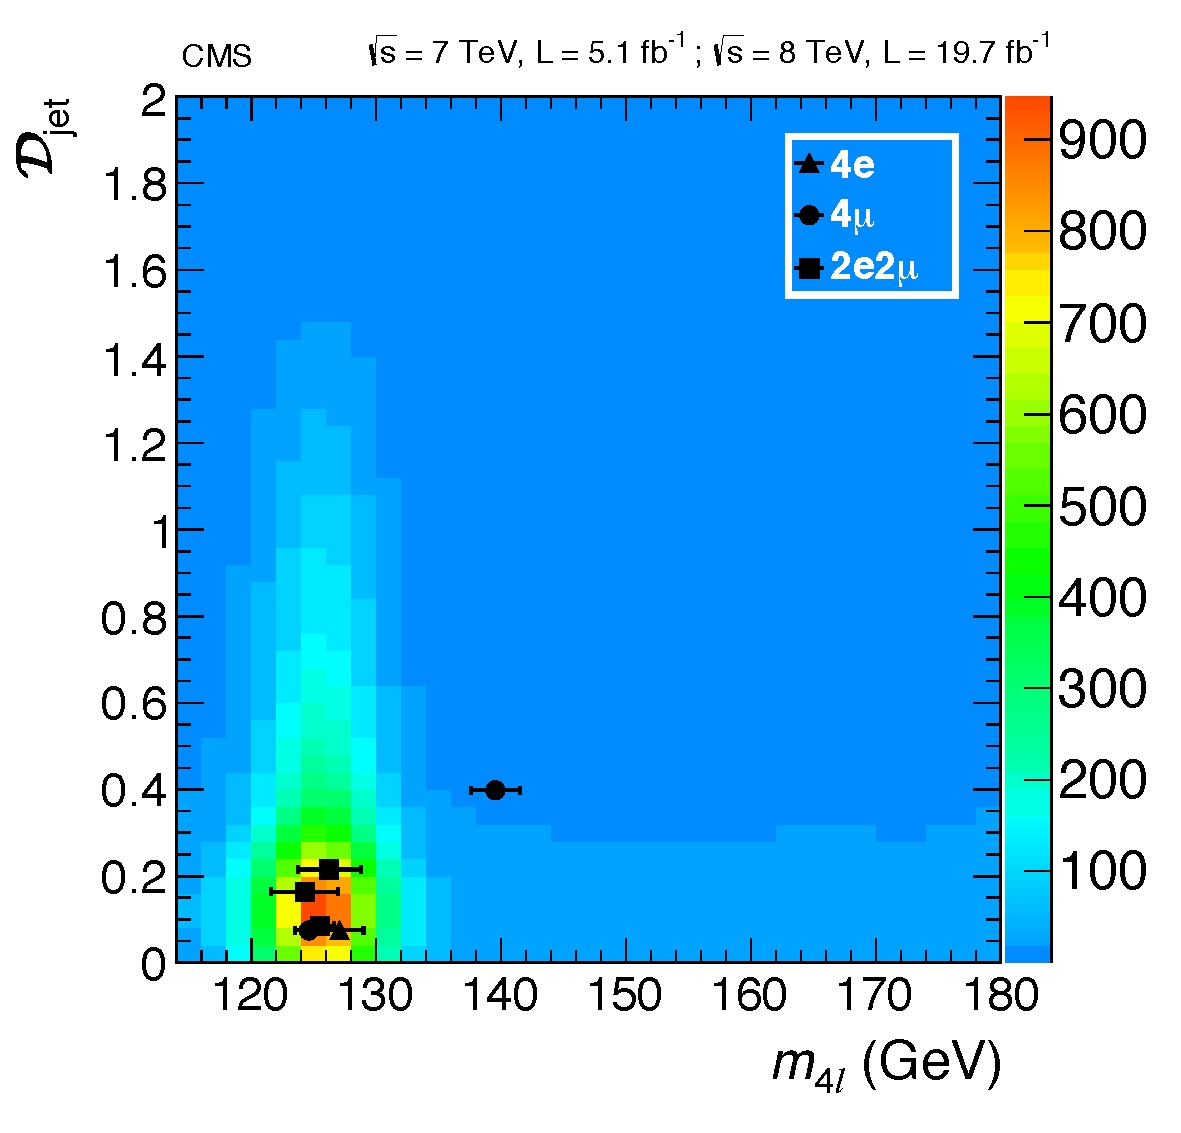
\includegraphics[width=0.45\textwidth]{HZZ4l_search/M4l_vs_Fisher_all.pdf}
    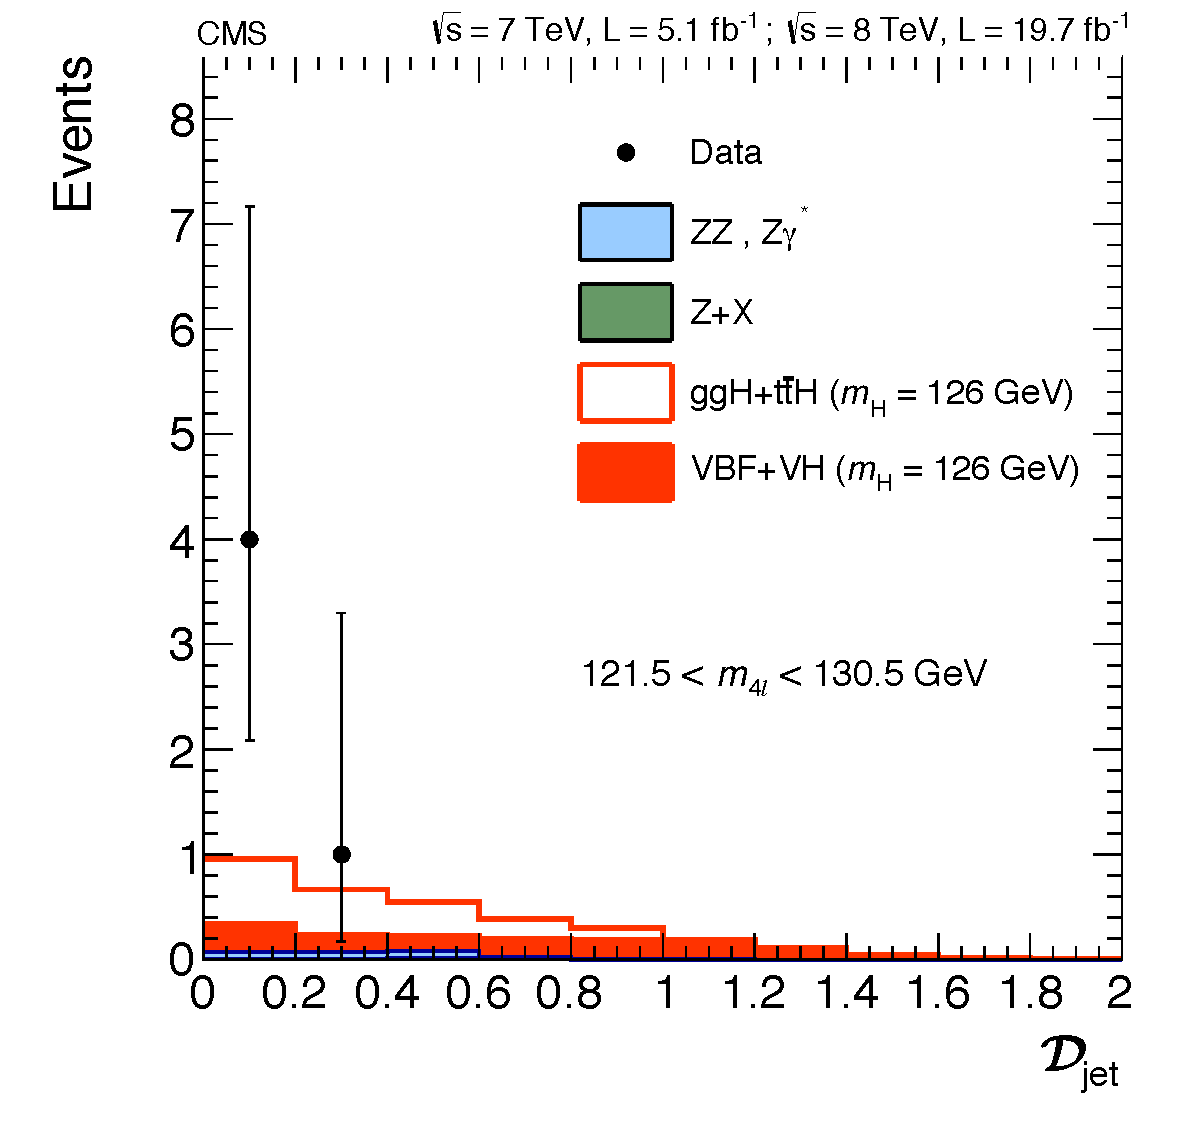
\includegraphics[width=0.45\textwidth]{HZZ4l_search/FisherPeak.pdf}
    \caption[(left) Distribution of $\mathcal{D}_{\text{jet}}$ versus $m_{4\ell}$ in the
      low-mass-range dijet category with colors shown for the expected
      relative density in linear scale (in arbitrary units) of
      background plus the Higgs boson signal for $m_H = \unit{126}{\GeV}$.  The
      points show the data and horizontal bars represent the measured
      mass uncertainties. (right) Distribution of $\mathcal{D}_{\text{jet}}$ in the dijet
      category for events in the mass region $121.5 < m_{4\ell} <
      \unit{130.5}{\GeV}$.  Points with error bars represent the data, shaded
      histograms represent the backgrounds, and the red histograms represent the
      signal expectation, broken down by production mechanism. Signal
      and background histograms are stacked.]{(left) Distribution of $\mathcal{D}_{\text{jet}}$ versus $m_{4\ell}$ in the
      low-mass-range dijet category with colors shown for the expected
      relative density in linear scale (in arbitrary units) of
      background plus the Higgs boson signal for $m_H = \unit{126}{\GeV}$.  The
      points show the data and horizontal bars represent the measured
      mass uncertainties. (right) Distribution of $\mathcal{D}_{\text{jet}}$ in the dijet
      category for events in the mass region $121.5 < m_{4\ell} <
      \unit{130.5}{\GeV}$.  Points with error bars represent the data, shaded
      histograms represent the backgrounds, and the red histograms represent the
      signal expectation, broken down by production mechanism. Signal
      and background histograms are stacked \cite{Chatrchyan:2013mxa}. \label{fig:FisherLow}}
  \end{center}
\end{figure}


\section{Search Results}
\label{sec:Search_Results}

In the low mass region of the analysis, an excess of events observed in the $4\ell$ mass spectrum localized in a narrow region in the vicinity of $\unit{126}{\GeV}$. The $m_{4\ell}$ distribution for the sum of the $4e$, $2e2\mu$, and $4\mu$ channels, in the mass region $70<m_{4\ell}<\unit{180}{\GeV}$, is shown in figure \ref{fig:Mass4lLow}. Around the observed peak, near $m_{4\ell} = \unit{126}{\GeV}$ the expected and observed candidate event yields are given in table \ref{tab:PreFitYieldsSigRegion}. Split into the categories according to the number of jets in the final state, in addition to the final state leptons, the expected and observed number of collision events is seen in table \ref{tab:PreFitYieldsSigRegionCat}.



\begin{figure}
  \begin{center} 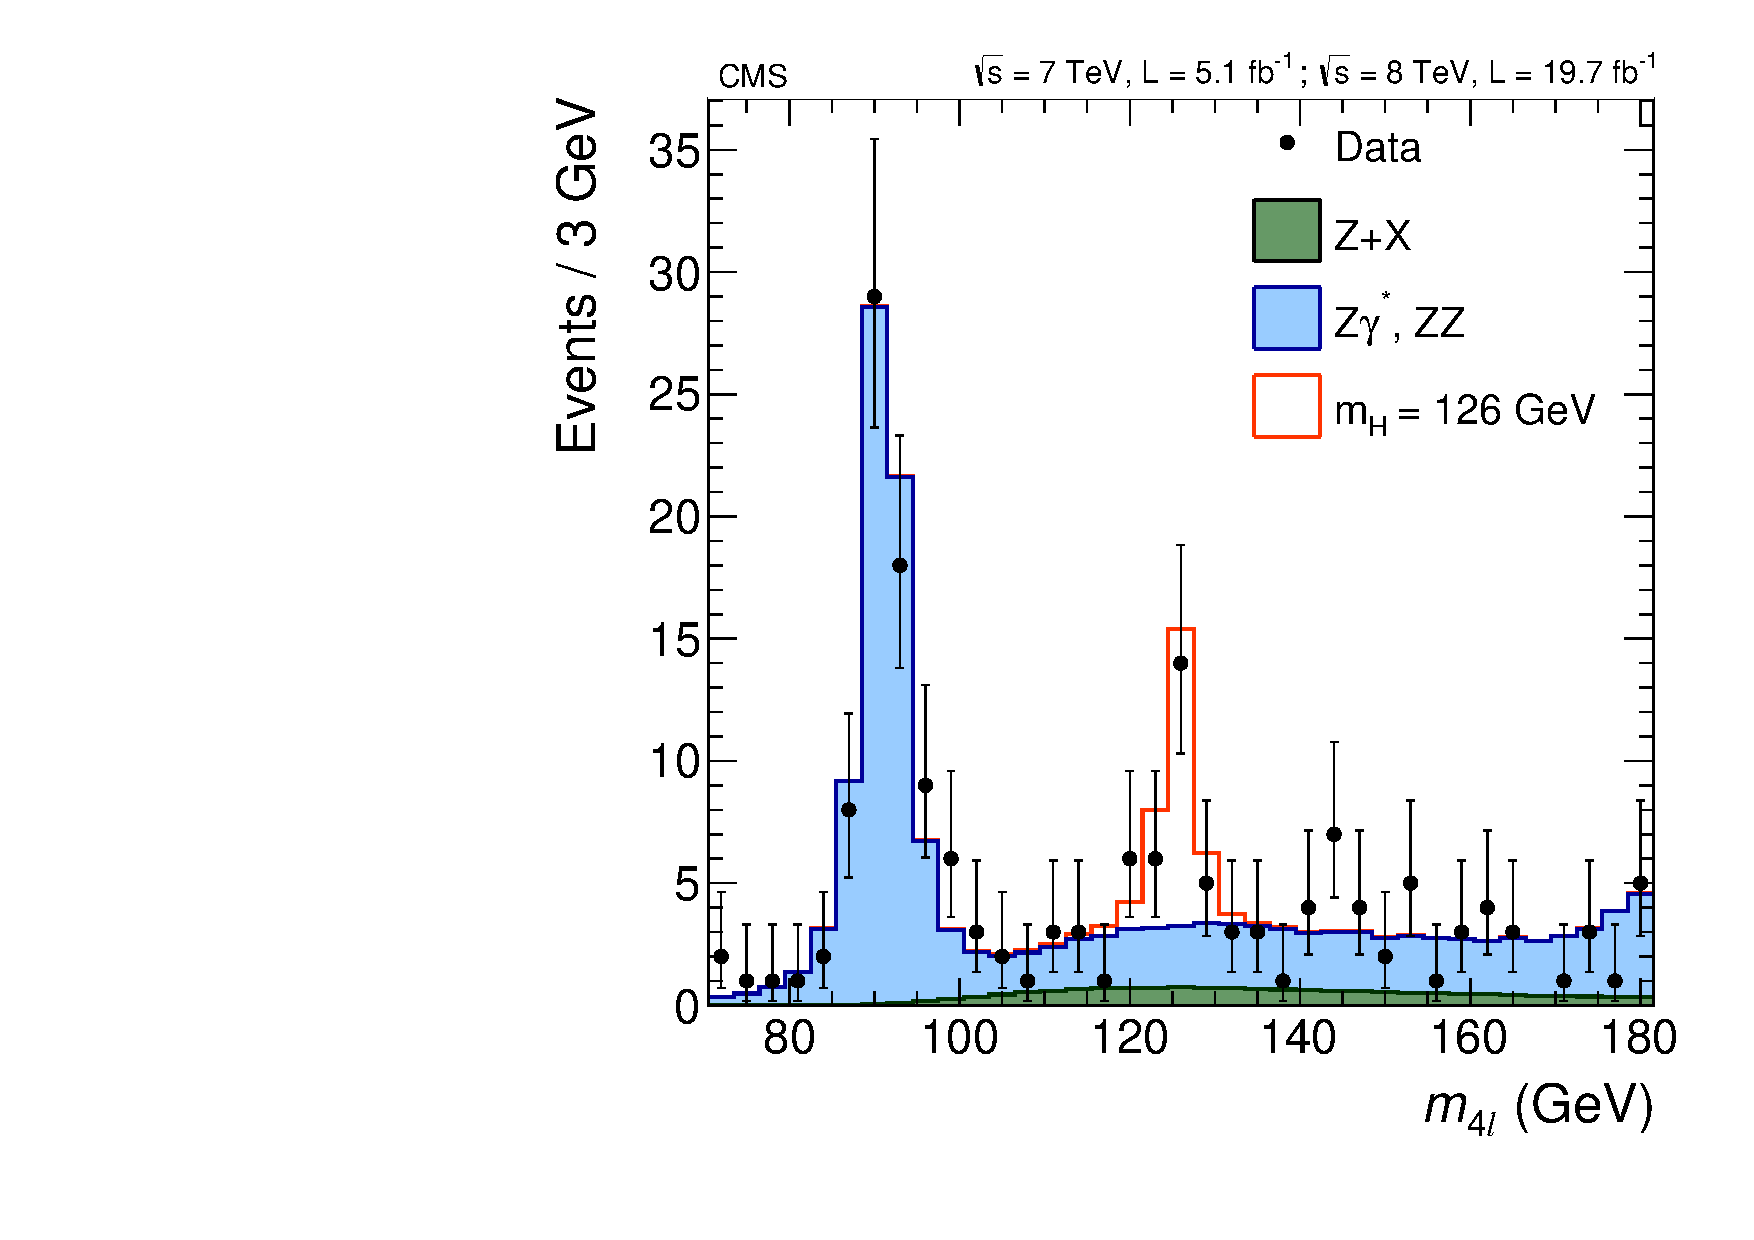
\includegraphics[width=0.75\linewidth]{HZZ4l_search/ZZMass_7Plus8TeV_70-180_3GeV.pdf}
   \caption[Distribution of the four-lepton reconstructed mass for the
    sum of the $4e$, $2e2\mu$, and $4\mu$ channels for the mass
    region $70<m_{4\ell}<\unit{180}{\GeV}$.  Points with error bars represent
    the data, shaded histograms represent the backgrounds, and the
    unshaded histogram represents the signal expectation for a mass hypothesis of
    $m_{H} = \unit{126}{\GeV}$. Signal and the $ZZ$ background are normalized to
    the SM expectation, the $Z+\text{jets}$ background to the estimation from
    data.]{Distribution of the four-lepton reconstructed mass for the
    sum of the $4e$, $2e2\mu$, and $4\mu$ channels for the mass
    region $70<m_{4\ell}<\unit{180}{\GeV}$.  Points with error bars represent
    the data, shaded histograms represent the backgrounds, and the
    unshaded histogram represents the signal expectation for a mass hypothesis of
    $m_{H} = \unit{126}{\GeV}$. Signal and the $ZZ$ background are normalized to
    the SM expectation, the $Z+\text{jets}$ background to the estimation from
    data \cite{Chatrchyan:2013mxa}.  \label{fig:Mass4lLow}} \end{center}
\end{figure}

\begin{table}
  \begin{center}
    \caption[The number of observed candidate events compared to the
      mean expected background and signal rates for each final state.
      Uncertainties include statistical and systematic sources.  The results
      are integrated over the mass range from 121.5 to $\unit{130.5}{\GeV}$ and for 7
      and $\unit{8}{\TeV}$ data combined.]{ The number of observed candidate events compared to the
      mean expected background and signal rates for each final state.
      Uncertainties include statistical and systematic sources.  The results
      are integrated over the mass range from 121.5 to $\unit{130.5}{\GeV}$ and for 7
      and $\unit{8}{\TeV}$ data combined \cite{Chatrchyan:2013mxa}.}
      \label{tab:PreFitYieldsSigRegion}
    \begin{tabular}{lcccc}
      Decay Channel        & $4e$ & $2e2\mu$ & $4\mu$  & $4\ell$ \\
      \hline
      $ZZ$ background &  1.1  $\pm$  0.1  &  3.2  $\pm$  0.2  &  2.5  $\pm$  0.2  &  6.8 $\pm$ 0.3  \\
      $Z + \text{jets}$ background &  0.8  $\pm$  0.2  &  1.3  $\pm$  0.3  &  0.4  $\pm$  0.2  &  2.6 $\pm$ 0.4 \\
      \hline
      All backgrounds            &  1.9  $\pm$  0.2   &  4.6  $\pm$ 0.4  & 2.9  $\pm$ 0.2  & 9.4  $\pm$ 0.5\\
      \hline
      $m_{H} =  \unit{125}{\GeV}$ &  3.0  $\pm$  0.4  &  7.9  $\pm$  1.0  &  6.4  $\pm$  0.7  & 17.3  $\pm$ 1.3 \\
      $m_{H} =  \unit{126}{\GeV}$ &  3.4  $\pm$  0.5  &  9.0  $\pm$  1.1  &  7.2  $\pm$  0.8  & 19.6  $\pm$ 1.5 \\
      \hline
      Observed  & 4 & 13 & 8 & 25 \\
    \end{tabular}
  \end{center}
\end{table}

\begin{table}
  \begin{center}
    \caption[The number of observed candidate events compared to the
      mean expected background and signal rates for the sum of the three
      final states for each of the two analysis categories.
      Uncertainties include statistical and systematic sources.  The
      results are integrated over the mass range from 121.5 to $\unit{130.5}{\GeV}$
      and for 7 and $\unit{8}{\TeV}$ data combined.  The expected signal yield for a
      SM Higgs boson with $m_{H} = \unit{126}{\GeV}$ is reported, broken down by the
      production mechanism.]{ The number of observed candidate events compared to the
      mean expected background and signal rates for the sum of the three
      final states for each of the two analysis categories.
      Uncertainties include statistical and systematic sources.  The
      results are integrated over the mass range from 121.5 to $\unit{130.5}{\GeV}$
      and for 7 and $\unit{8}{\TeV}$ data combined.  The expected signal yield for a
      SM Higgs boson with $m_H = \unit{126}{\GeV}$ is reported, broken down by the
      production mechanism \cite{Chatrchyan:2013mxa}.}
      \label{tab:PreFitYieldsSigRegionCat}
    \begin{tabular}{lcc}
      Category       & 0/1-jet  &   Dijet  \\
      \hline
      $ZZ$ background &  6.4  $\pm$  0.3  &  0.38 $\pm$  0.02  \\
      $Z + \text{jets}$ background &  2.0  $\pm$  0.3  &  0.5  $\pm$  0.1  \\
      \hline
      All backgrounds       &  8.5  $\pm$  0.5  &  0.9  $\pm$ 0.1 \\
      \hline
      $gg \to H$               &  15.4 $\pm$  1.2   &   1.6  $\pm$  0.3 \\
      $t\bar{t} \to H$           &         NA          &  0.08  $\pm$  0.01 \\
      VBF                   &  0.70 $\pm$  0.03  &  0.87  $\pm$  0.07 \\
      $WH$              &  0.28 $\pm$  0.01  &  0.21  $\pm$  0.01 \\
      $ZH$             &  0.21 $\pm$  0.01  &  0.16  $\pm$  0.01 \\
      \hline
      All signal, $m_{H} = \unit{126}{\GeV}$            &  16.6 $\pm$  1.3  &  3.0  $\pm$  0.4 \\
      \hline
      Observed              & 20 & 5 \\
    \end{tabular}
  \end{center}
\end{table}


Experimental systematic uncertainties in the normalization of the signal and the irreducible background processes are evaluated from data for the trigger and the combined lepton reconstruction, identification, and isolation efficiencies. Data is used to validate the absolute momentum scale and resolution resulting in effects of $0.3\%\left(4e\right)$, $0.1\%\left(2e2\mu\right)$, and $0.1\%\left(4\mu\right)$ on the mass scale. The effect of the energy resolution uncertainties is taken into account by introducing a 20\% uncertainty in the simulated width of the signal mass peak, according to the maximum deviation between data and simulation observed in $Z \to \ell^{+}\ell^{-}$ events. Due to low statistics in the control regions systematic uncertainties of 20\%, 25\%, and 40\% are assigned to the normalization of the reducible background for the $4e$, $2e2\mu$, and $4\mu$ final states, respectively. The uncertainty in the luminosity measurement
(2.2\% at $\unit{7}{\TeV}$ and 2.6\% at $\unit{8}{\TeV}$) \cite{CMS-PAS-EWK-11-001, CMS-PAS-LUM-13-001} is also applied to all hypothetical signals and backgrounds.

The theoretical uncertainties in the irreducible background are computed as functions of $m_{4\ell}$, varying both the renormalization and factorization scales and the parton distribution function set. Systematic uncertainties in the Higgs boson cross section and branching fraction are taken from \cite{Denner:2011mq, Dittmaier:2011ti}. In the 0/1-jet category, an additional background normalization is assigned to account for the differences in Monte Carlo predictions, while an additional signal systematics are assigned in the dijet category to account for cross section uncertainties in $H +\text{jets}$ and VBF production. A summary of the systematic uncertainties in the normalizations of the signal and background processes is given in table \ref{tab:systematics}.

\begin{table}
  \begin{center}
    \caption[Effect of systematic uncertainties on the yields of
      signal ($m_H = \unit{126}{\GeV}$) and background processes for the $\unit{8}{\TeV}$
      data set and 0/1-jet category. Uncertainties appearing on the same line are 100\% correlated, with two exceptions: those related to the missing higher orders are not correlated, and those from the $\alpha_S$ + PDF (gg) in $t\bar{t}H$ are 100\% anticorrelated. 
 Uncertainties for the $\unit{7}{\TeV}$ data set are similar.]{Effect of systematic uncertainties on the yields of
      signal ($m_H = \unit{126}{\GeV}$) and background processes for the $\unit{8}{\TeV}$
      data set and 0/1-jet category. Uncertainties appearing on the same line are 100\% correlated, with two exceptions: those related to the missing higher orders are not correlated, and those from the $\alpha_S$ + PDF (gg) in $t\bar{t}H$ are 100\% anticorrelated. 
 Uncertainties for the $\unit{7}{\TeV}$ data set are similar \cite{Chatrchyan:2013mxa}.
      \label{tab:systematics}}
    \begin{tabular}{lccccccc}
      Source         & \multicolumn{4}{c}{Signal ($m_H = \unit{126}{\GeV}$)}  &  \multicolumn{3}{c}{Backgrounds} \\
      \hline
      & $gg \to H$       & VBF     &  $VH$   &  $t\bar{t}H$ &  $q\bar{q} \to ZZ$  &  $gg \to ZZ$  & $Z+\text{jets}$ \\
      \hline
      $\alpha_S$ + PDF (gg)           & 7.2\%         &  \text{---}      &   \text{---}                  &  7.8\%       &  \text{---}                     &  7.2\%            & \text{---}  \\
      $\alpha_S$ + PDF ($q\bar{q}$)    & \text{---}             &  2.7\%  &   3.5\%               &  \text{---}           &  3.4\%                 &  \text{---}                & \text{---}   \\
      Higher orders           & 7.5\%         &  0.2\%  &  0.4\%, 1.6\%         & 6.6\%        &  2.9\%                 &  24\%             & \text{---}   \\
      Signal acceptance               & \multicolumn{4}{c}{ 2\% }                                      &  \text{---}                     & \text{---}                 & \text{---}   \\
      BR($H \to ZZ$)              & \multicolumn{4}{c}{ 2\% }                                      &  \text{---}                     &  \text{---}                 & \text{---}   \\
      Luminosity                      & \multicolumn{6}{c}{ 2.6\% }                                                                                 & \text{---}   \\
      Electron efficiency             & \multicolumn{6}{c}{ 10\% ($4e$),   4.3\% ($2e2\mu$)}                                                 & \text{---}   \\
      Muon efficiency                 & \multicolumn{6}{c}{ 4.3\% ($4\mu$), 2.1\% ($2e2\mu$)}                                                 & \text{---}   \\
      Control region                  & \text{---}             & \text{---}       & \text{---}                     & \text{---}            & \text{---}                      & \text{---}                 & 40\% \\
    \end{tabular}
  \end{center}
\end{table}

Shape uncertainties are applied to all three kinematic distributions used in the analysis. In the $m_{4\ell}$ dimension shape variations are used to account for variations due to  the lepton scale and resolution impacts. In the $\mathcal{D}^{\text{kin}}_{\text{bkg}}$ dimension shape variations are used for the uncertainty in the $Z + \text{jets}$ shape. In the 0/1-jet category the $p_{T}^{4\ell}$ shape is assigned a systematic to account for the theoretical uncertainty in the shape. Both theoretical and experimental (jet energy scale and resolution) shape systematics are assigned to the $\mathcal{D}_{\text{jet}}$ distribution.

\subsection{Quantifying the observation}

To quantify this observation and to account for all the necessary uncertainties in our analysis procedure a three-dimensional unbinned miximim-likelihood fit is performed on the selected collision events. The fits include probability density functions for five signal components (gluon fusion, VBF, $WH$, $ZH$, and $t\bar{t}H$ productions) and three background processes ($q\bar{q} \to ZZ$, $gg \to ZZ$, and $Z+ \text{jets}$). The normalizations of these components and systematic uncertainties are introduced in the fits as nuisance parameters, assuming log-normal {\it a priori} probability distributions, and are profiled during the minimization. The shapes of the probability density functions for the event observables are also varied within alternative shapes as experimental or theoretical systematic uncertainties.

The three main questions for the analysis to quantitatively answer are: 
\begin{itemize}
\item[(1)] What Higgs boson hypotheses can we exclude? 
\item[(2)] What is the statistical significance of any observed deviation from the SM expectations? 
\item[(3)] Does the measured cross section times branching ratio match the SM Higgs boson expectation? 
\end{itemize}
The likelihood that is used to address these questions is given in equation \eqref{eq:3D_likelihood} where $m_{H}, \Gamma$ are the Higgs boson mass and width and the other discriminants are defined in the previous section. In total, the selected events are split into twelve subcategories based on the three final states, two data-taking periods (7 \& $\unit{8}{\TeV}$), and two jet categories. The events are examined for 187 hypothetical SM-like Higgs boson masses in a range between 110 and $\unit{1000}{\GeV}$.

\begin{eqnarray}
\label{eq:3D_likelihood}
\mathcal{L}_{3D}^{\mu} \equiv& \mathcal{L}_{3D}^{\mu,\,\text{0/1-jet}}(m_{4\ell},\mathcal{D}^\text{kin}_\text{bkg},p_{T}^{4\ell})
           =&
            \mathcal{P}(m_{4\ell}|m_{H},\Gamma)
            \mathcal{P}(\mathcal{D}^\text{kin}_\text{bkg}|m_{4\ell})
            \mathcal{P}(p_{T}^{4\ell}|m_{4\ell}) \\
    \label{eqn:likmu_2j}
\mathcal{L}_{3D}^{\mu} \equiv& \mathcal{L}_{3D}^{\mu,\,\text{Dijet}}(m_{4\ell},\mathcal{D}^\text{kin}_\text{bkg},\mathcal{D}_\text{jet})
           =&
            \mathcal{P}(m_{4\ell}|m_{H},\Gamma)
            \mathcal{P}(\mathcal{D}^\text{kin}_\text{bkg}|m_{4\ell})
            \mathcal{P}(\mathcal{D}_\text{jet}|m_{4\ell}) \nonumber 
\end{eqnarray}



Question (1) is answered by fitting the data for exclusion limits as a function of the Higgs boson hypothesis mass $m_{H}$. Exclusion limits are determined by fitting the data using the $\mathrm{CL_{s}}$ frequentist construction \cite{Junk:1999kv,Read:2002hq} to determine the range of masses that are excluded at 95\% confidence level (C.L.). Generally, this is done by fitting both data, under the assumption of a specific Higgs boson mass $m_{H}$, and many pseudo-datasets for the \textit{signal strength} $\left(\mu = \sigma/\sigma_{SM}\right)$, the ratio of the observed and expected SM cross section times branching ratio. Once the fit to data is performed, the 95\% confidence level (C.L.) upper limit on $\mu$ is determined from the distribution of pseudo-data experiments. When this upper limit gives $\mu >1$ the data is consistent (within 95\%) with both signal+background and background only hypotheses at that mass $m_{H}$. The region where the upper limit is at a $\mu < 1$ is the \textit{excluded range} where the data to a 95\% C.L. excludes the signal+background hypothesis at that mass.

The result of the 187 fits of the $\mathcal{L}_{3D}^{\mu}$ likelihood are shown in figure \ref{fig:ExclusionLimits}. Here one can see the observed 95\% C.L. upper limit on $\mu$ for each mass point. Additionally the median, $\pm1\sigma$, and $\pm2\sigma$ expected exclusion for background-only fit are shown as a dashed line, green band, and yellow bands respectively. From this plot, Higgs boson hypotheses with masses $m_{H} \in \left[\unit{115--750}{\GeV}\right]$ were expected to be excluded at a 95\% C.L. using the four-lepton final state, a large fraction of the $\unit{110--1000}{\GeV}$ analysis range. From the observed number of events, bosons with masses between $\unit{114.5--119.0}{\GeV}$ and $\unit{129.5--832.0}{\GeV}$ can actually be excluded at a 95\% C.L. using the four-lepton final state. The unexcluded region between $m_{H} \in \unit{119.0--129.5}{\GeV}$ corresponds to the excess that is seen in figure \ref{fig:Mass4lLow}.

\begin{figure}
  \begin{center} 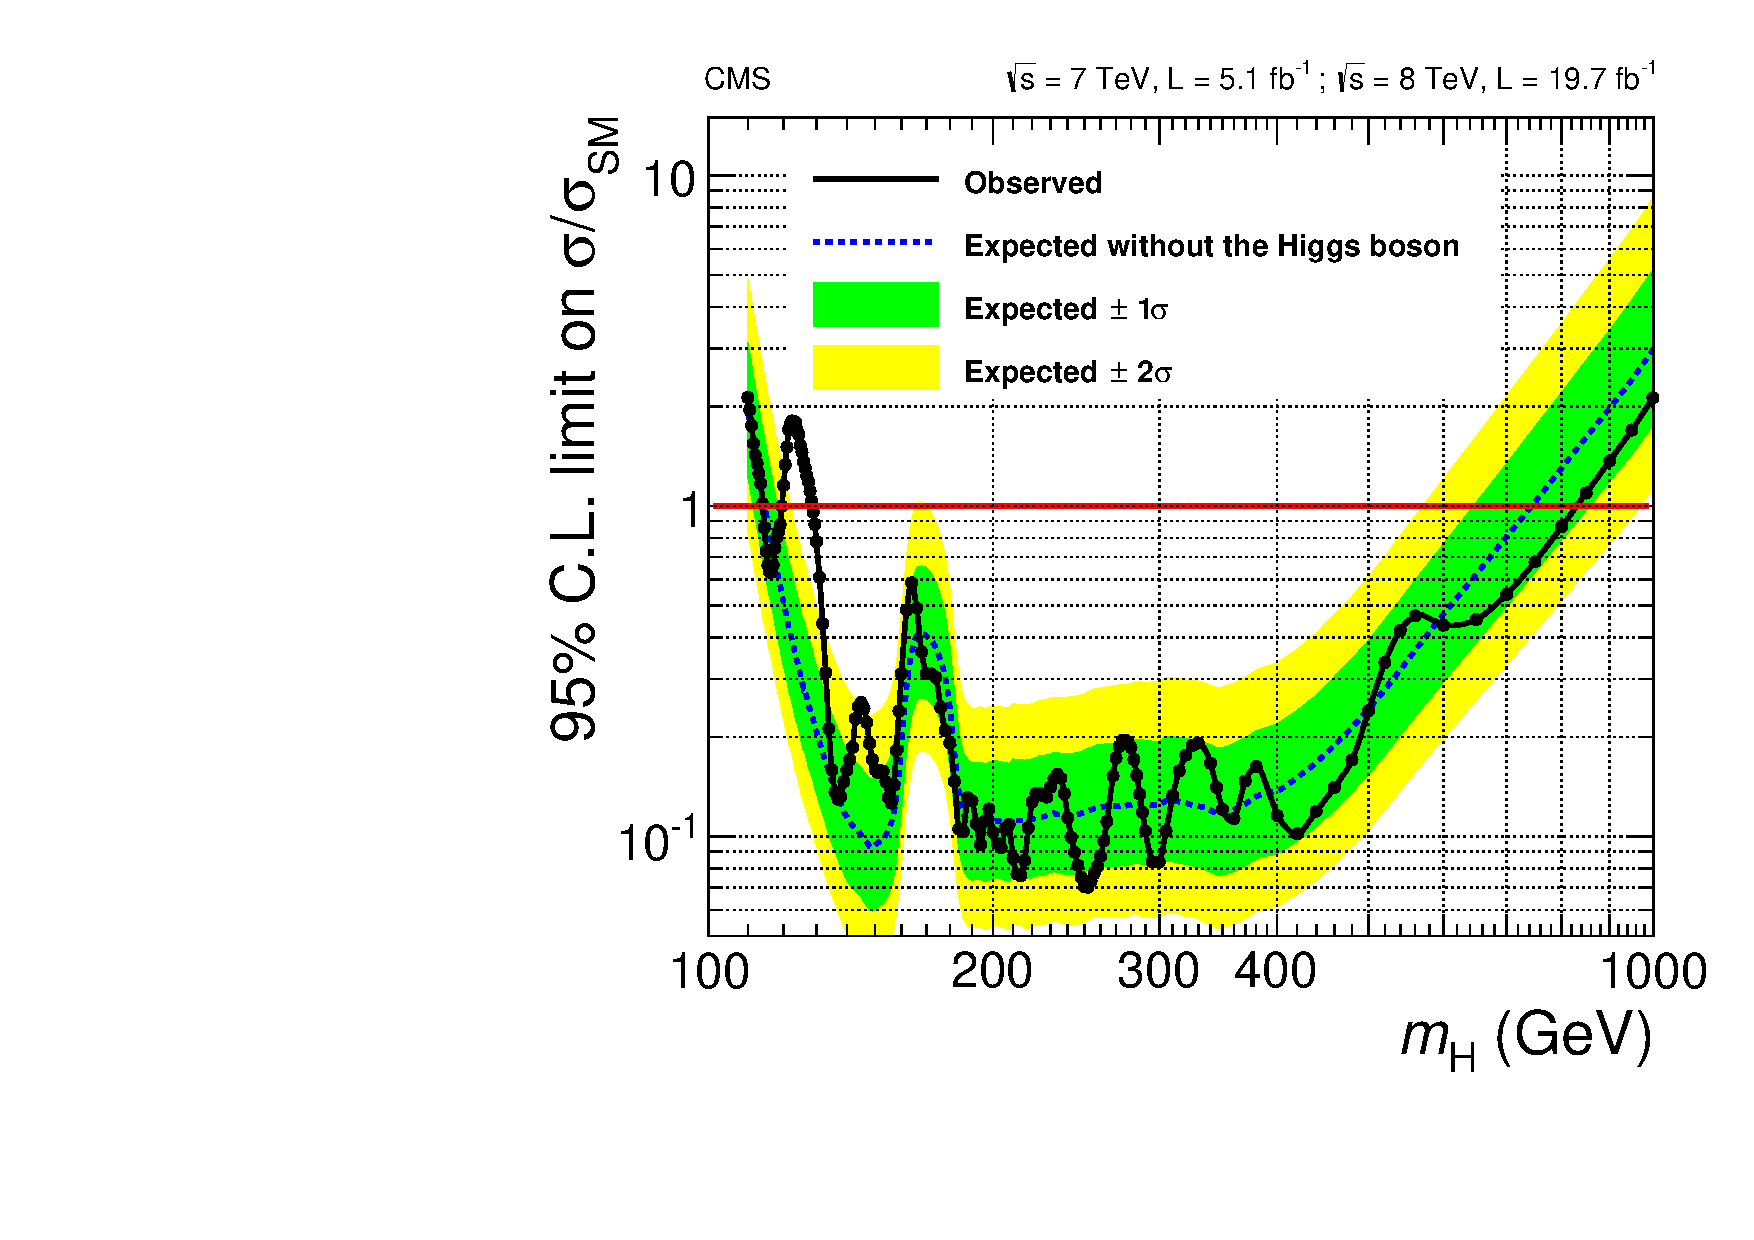
\includegraphics[width=0.75\linewidth]{HZZ4l_search/UpperLimit_ASCLS_7p8TeV_wholeMass_Final2_2l2tau.pdf}
   \caption[Observed and expected 95\% C.L. upper limit on the ratio of the production cross section to the SM expectation. The expected $\pm1\sigma$ and $\pm2\sigma$ C.L. ranges of expectation for the background-only model are also shown with green and yellow bands, respectively. ]{Observed and expected 95\% C.L. upper limit on the ratio of the production cross section to the SM expectation. The expected $\pm1\sigma$ and $\pm2\sigma$ C.L. ranges of expectation for the background-only model are also shown with green and yellow bands, respectively \cite{Chatrchyan:2013mxa}.  \label{fig:ExclusionLimits}} \end{center}
\end{figure}


Question (2) is answered by computing the local p-value from the $\mathcal{L}_{3D}^{\mu}$ likelihood, these represent the the significance of a local excess relative to the background expectation, are shown for the full mass range as a function $m_{H}$ in figure \ref{fig:p-value} (left) and near the peak in figure \ref{fig:p-value} (right). The minimum of the local p-value is reached around $m_{4\ell} = \unit{125.7}{\GeV}$, and corresponds to a local significance of $6.8\sigma$, consistent with the expected sensitivity of $6.7\sigma$. These values measure the number of standard deviations that the median background distributions would have to fluctuate in order to `fake' the signal that we observe. 

As a cross-check, 1D [$\mathcal{L}_{1D}^{\mu} \equiv \mathcal{L}_{1D}^{\mu}(m_{4\ell})$] and 2D [$\mathcal{L}_{2D}^{\mu} \equiv \mathcal{L}_{2D}^{\mu}(m_{4\ell},\mathcal{D}^\text{kin}_\text{bkg})$] models are also studied, as shown in figures \ref{fig:p-value} (left) and (right), resulting in an observed local significance of $5.0$$\sigma$ and $6.9$$\sigma$, for an expectation of $5.6$$\sigma$ and $6.6$$\sigma$, respectively. These results are consistent with the 3D model; however, with a systematically lower expected sensitivity to the signal. No other significant deviations with respect to the expectations is found in the mass range $\unit{110--1000}{\GeV}$. All of these results are consistent with previous CMS and ATLAS publications \cite{Aad:2012tfa, Chatrchyan:2012ufa, Chatrchyan:2013lba}, and the second most significant p-value minimum is reached around $m_{4\ell} = \unit{146}{\GeV}$, with a local significance of $2.7\sigma$. This computation does not take into account the look-elsewhere effect~\cite{Gross:2010qma}.

\begin{figure}
  \begin{center} 
  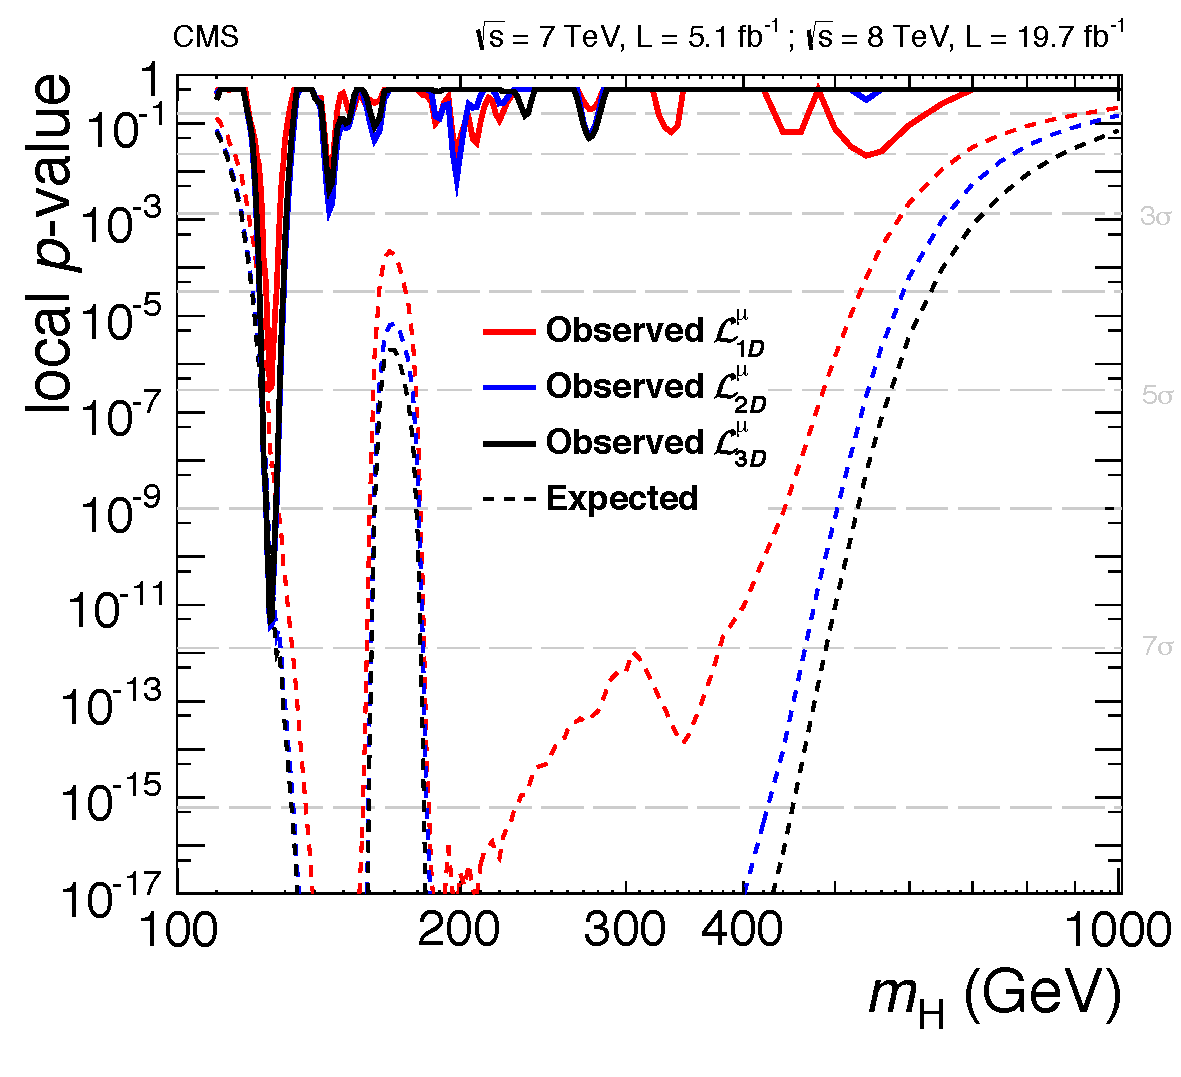
\includegraphics[width=0.45\linewidth]{HZZ4l_search/Pvals_PLP_wholeMass_Final3_2l2tau_7p8sep.pdf}
  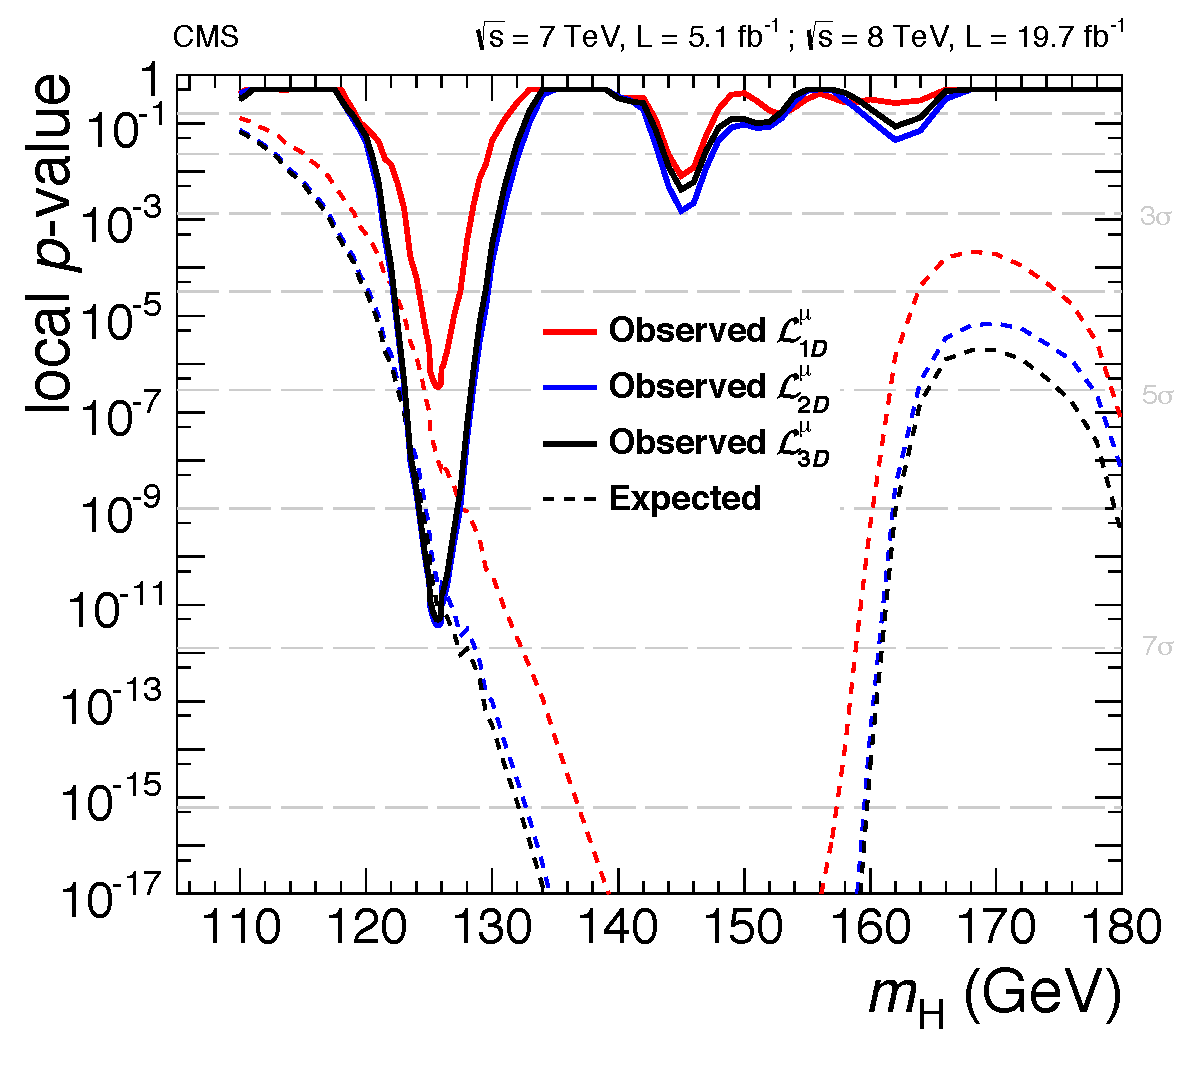
\includegraphics[width=0.45\linewidth]{HZZ4l_search/Pvals_PLP_lowMass_1D2D3D_Final3_no2l2tau_7p8sep.pdf}
   \caption[(left) Significance of the local excess with respect to the SM background expectation as a function of the Higgs boson mass in the full mass range $\unit{110--1000}{\GeV}$. Results obtained using the 1D fit, 2D fit, and the nominal 3D fit. (right) Significance of the local excess with respect to the SM background expectation as a function of the Higgs boson mass for the 1D fit, 2D fit, and the nominal 3D fit. Results are shown for the full data sample in the low-mass region only.]{(left) Significance of the local excess with respect to the SM background expectation as a function of the Higgs boson mass in the full mass range $\unit{110--1000}{\GeV}$. Results obtained using the 1D fit, 2D fit, and the nominal 3D fit. (right) Significance of the local excess with respect to the SM background expectation as a function of the Higgs boson mass for the 1D fit, 2D fit, and the nominal 3D fit. Results are shown for the full data sample in the low-mass region only \cite{Chatrchyan:2013mxa}.  \label{fig:p-value}} \end{center}
\end{figure}

As a validation of this thesis work, plots were also made of the signal to background ratio from each of the likelihood models (1D, 2D, 3D). These distributions are shown in figure \ref{fig:sig_bkg} where the background components are given in the filled histograms, the outline provides the expectation for signal, and the observed events are shown as data points. A Higgs boson hypothesis of $m_{H} = \unit{126}{\GeV}$ is used and the plots are made from the $m_{4\ell} \in\unit{121.5--130.5}{\GeV}$ region to study the observed peak. One can see that with each additional dimension added to the likelihood the separation between the signal and background increases. 

\begin{figure}
  \begin{center} 
  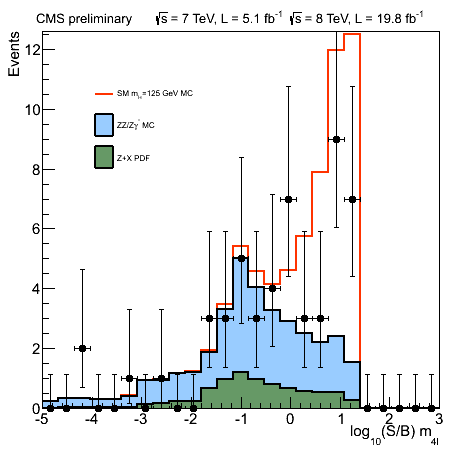
\includegraphics[width=0.3\linewidth]{HZZ4l_search/1D_new.png}
  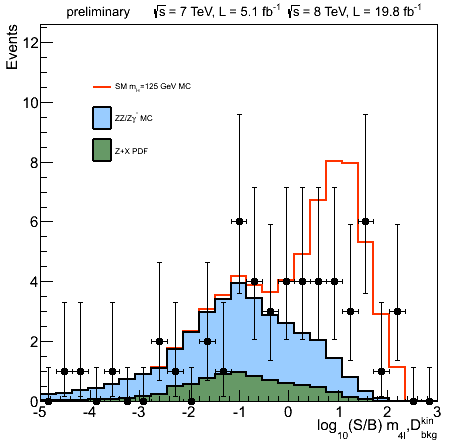
\includegraphics[width=0.3\linewidth]{HZZ4l_search/2D_new.png}
  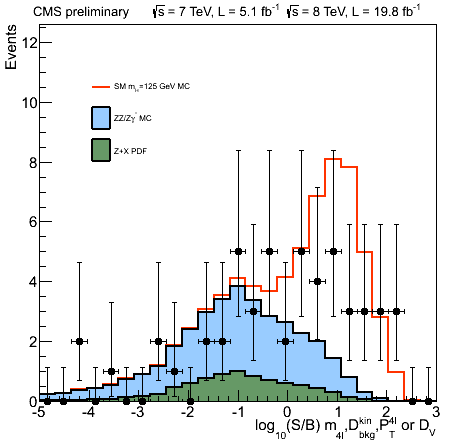
\includegraphics[width=0.3\linewidth]{HZZ4l_search/3D_new.png}
   \caption[Signal to background ratio's for expected and observed events, computed from the 1D (left), 2D (left), and 3D (right) likelihoods. These plots are made from the $m_{4\ell} \in\unit{121.5--130.5}{\GeV}$ region to study the observed peak. The signal used as the Higgs boson hypothesis corresponds to $m_{H} = \unit{126}{\GeV}$.These plots are preliminary and unpublished.]{Signal to background ratio's for expected and observed events, computed from the 1D (left), 2D (left), and 3D (right) likelihoods. These plots are made from the $m_{4\ell} \in\unit{121.5--130.5}{\GeV}$ region to study the observed peak. The signal used as the Higgs boson hypothesis corresponds to $m_{H} = \unit{126}{\GeV}$.These plots are preliminary and unpublished.  \label{fig:sig_bkg}} \end{center}
\end{figure}

Question (3) asks if the observations we see are consistent with the SM Higgs boson that is predicted. Using the signal strength $\left(\mu = \sigma/\sigma_{SM}\right)$ we have already defined we can quantify this. If the likelihoods minimize giving $\mu = 1$ then the data is consistent with the Higgs boson. All of these studies are performed at the best fit mass for the Higgs boson using this $4\ell$ final state, $m_{H} = \unit{125.6}{\GeV}$ \cite{Chatrchyan:2013mxa}. By fitting the signal expectations we can estimate the sensitivity based on the systematics and statistics currently available. Such a fit of the expected results gives a median expected signal strength of $\mu = 1.00^{+0.31}_{-0.26}$. The fit of the actual data gives $\mu = 0.93^{+0.26}_{-0.23}\text{(stat.)} ^{+0.13}_{-0.09}\text{(syst.)}$ in very good agreement with the SM Higgs boson expectations. This fit also illuminates that the statistical and systematic uncertainties are of the same order of magnitude, spointing to the need for increased study of systematic uncertainties in future studies.

\subsection{Search for additional Higgs bosons}

Using a preliminary unpublished version of the analysis, where a Higgs boson of $m_{H} = \unit{126}{\GeV}$ is added to the background instead of the signal, this thesis work searched the data in the four-lepton final state for additional bosons that might be observed. In BSM models that have more than one Higgs boson the four-lepton final state may see both of these bosons. In regions far away from the new peak the limits shown in figure \ref{fig:ExclusionLimits} are valid. Near the peak, we can recreate the likelihoods with the new $\unit{126}{\GeV}$ Higgs background process and perform a search for a second peak (identical to a SM Higgs boson) near or under the observed one. These results can be seen in figure \ref{fig:ExclusionLimits_2H} where no additional boson is seen. Additionally, the local significance for a (Higgs boson identical) BSM boson is shown and no significant deviation from the background is seen.

\begin{figure}
  \begin{center} 
  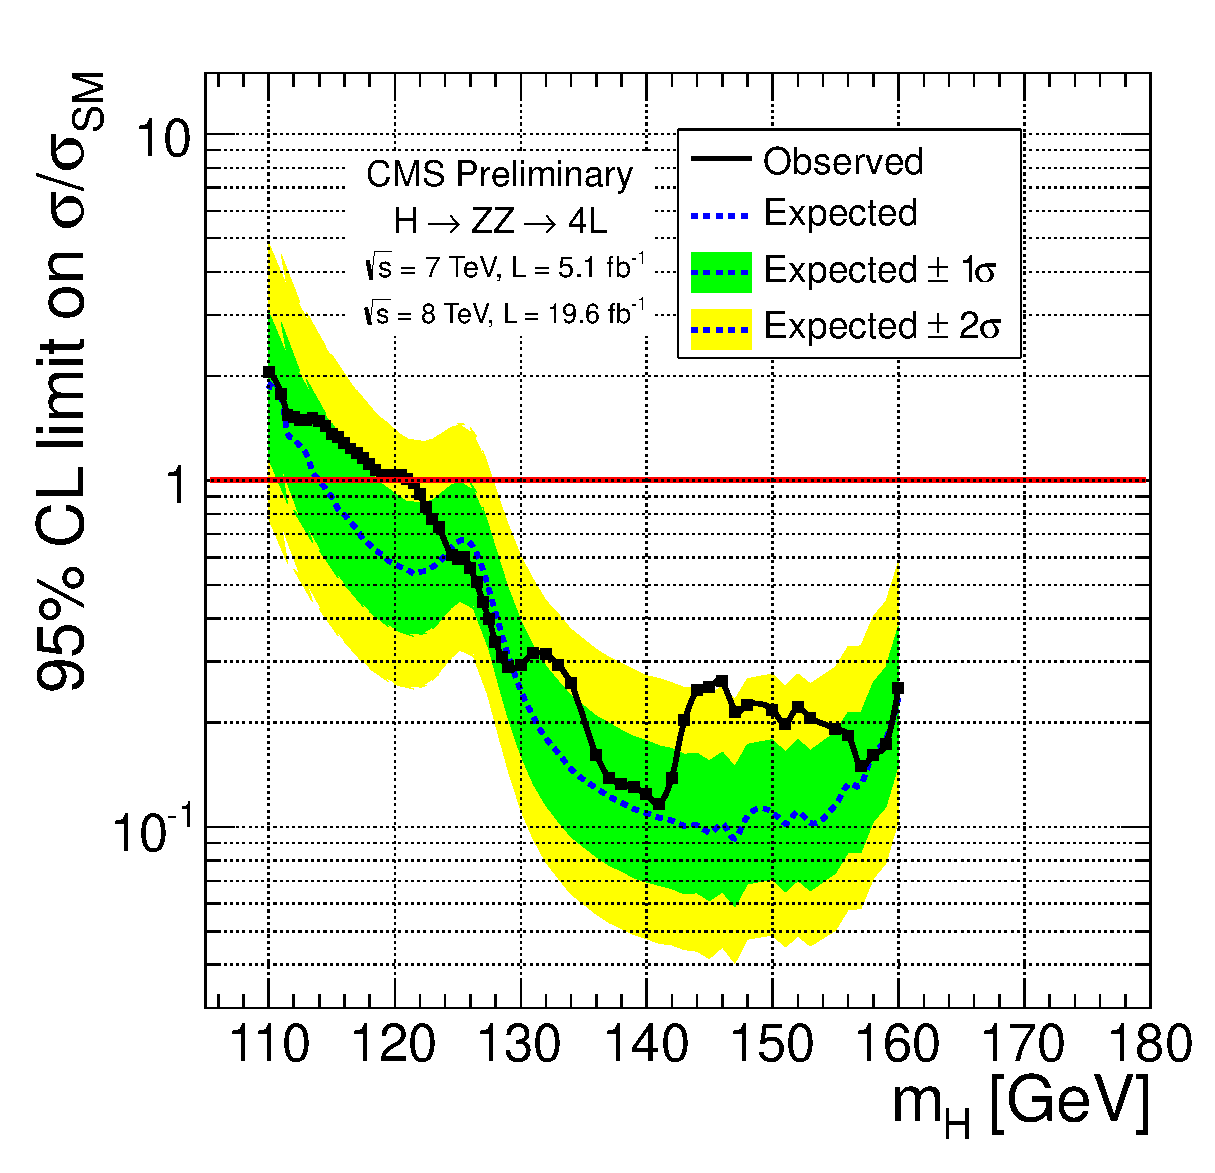
\includegraphics[width=0.45\linewidth]{HZZ4l_search/UpperLimit_ASCLS_7p8TeV_lowMass_2H_search.eps}
  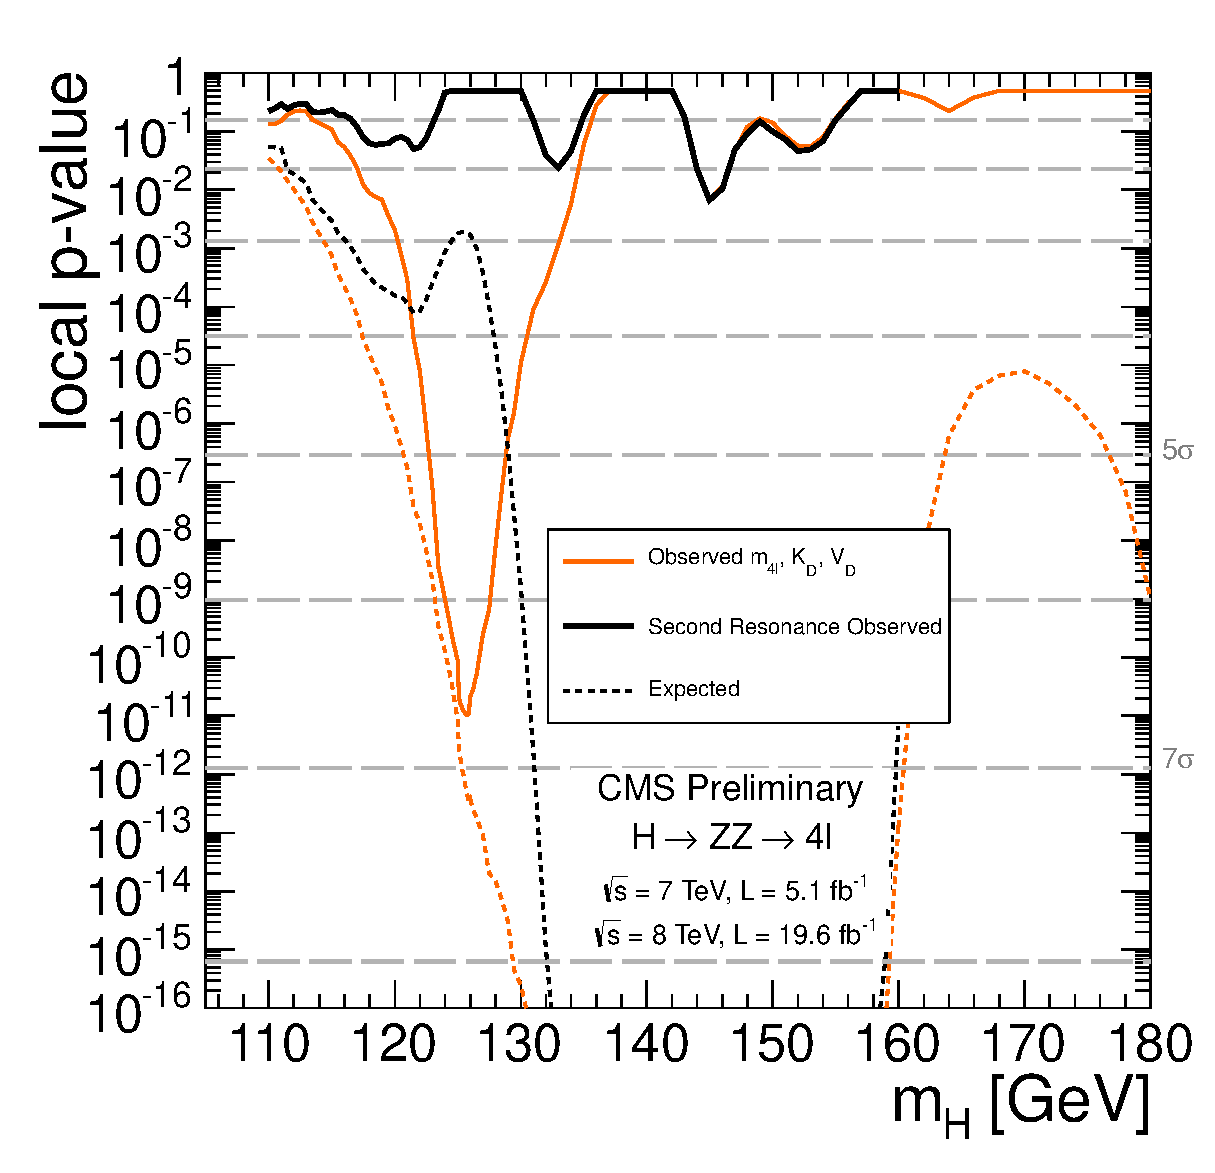
\includegraphics[width=0.45\linewidth]{HZZ4l_search/Pvals_PLP_lowMass_2H_no2l2tau_7p8sep.eps}
   \caption[(left) Observed and expected 95\% C.L. upper limit on the ratio of the production cross section to the SM expectation where a $\unit{126}{\GeV}$ Higgs boson is added as background. The expected $\pm1\sigma$ and $\pm2\sigma$ C.L. ranges of expectation for the background-only model are also shown with green and yellow bands, respectively. (right) Significance of the local excess with respect to the SM background + $\unit{126}{\GeV}$ Higgs boson expectation as a function of the BSM Higgs boson mass and compared to the expected and observed significance of the SM Higgs boson. These results were obtained from a preliminary version of the $4\ell$ analysis and are unpublished.]{(left) Observed and expected 95\% C.L. upper limit on the ratio of the production cross section to the SM expectation where a $\unit{126}{\GeV}$ Higgs boson is added as background. The expected $\pm1\sigma$ and $\pm2\sigma$ C.L. ranges of expectation for the background-only model are also shown with green and yellow bands, respectively. (right) Significance of the local excess with respect to the SM background + $\unit{126}{\GeV}$ Higgs boson expectation as a function of the BSM Higgs boson mass and compared to the expected and observed significance of the SM Higgs boson. These results were obtained from a preliminary version of the $4\ell$ analysis and are unpublished.  \label{fig:ExclusionLimits_2H}} \end{center}
\end{figure}


\section{Production \& Decay Fraction Results}
\label{sec:prod_dec_frac}

Looking at the results presented in the previous section, the addition of the $p_{T}^{4\ell}$ and $\mathcal{D}_{\text{jet}}$ shapes don't add too much to the sensitivity of the search. However these distributions allow the three-dimensional likelihood to be sensitive to the production \& decay fractions of the Higgs boson.

To investigate these quantities, modified definitions of the signal strength are used. These modified quantities measure the ratio of the interesting cross section times branching ratio to the SM expectation for this value. In this way, $\mu_{\text{X}} = 1$ is the standard model, while a $\mu_{\text{X}}$ inconsistent with 1 would be a sign of non-SM behavior.

The decay fraction results are reported in two categories, 0/1-jet and dijet. These results are presented in figure \ref{fig:mucat} (left). The vertical blue line, and green band shows the combined $\mu$ fit presented in the last section, while the black points and red horizontal bars indicate the fit of the signal strength in the two individual categories. The result is $\mu_{\text{0/1-jet}} = 0.83^{+0.31}_{-0.25}$ in the 0/1-jet category and $\mu_{\text{dijet}} = 1.45^{+0.89}_{-0.62}$ in the dijeft category. for each category, the signal strength is consistent with SM expectations within the uncertainties, which are dominated by statistical uncertainties.

To disentangle the production mechanisms of the observed new state, the production mechanisms are split into two families depending on whether the production is through couplings to fermions (gluon fusion, $t\bar{t}H$) or vector bosons (VBF, $VH$).  For $m_{H} = \unit{126}{\GeV}$, about 55\% of the VBF events are expected to be included in the dijet category, while only 8\% of the gluon fusion events are included in the dijet category. As shown in table~\ref{tab:PreFitYieldsSigRegionCat}, a fraction of 43\% of $WH$ and $ZH$ production contributes to the dijet category. Events that contribute are those in which the vector boson decays hadronically.

\begin{figure}
  \begin{center}
    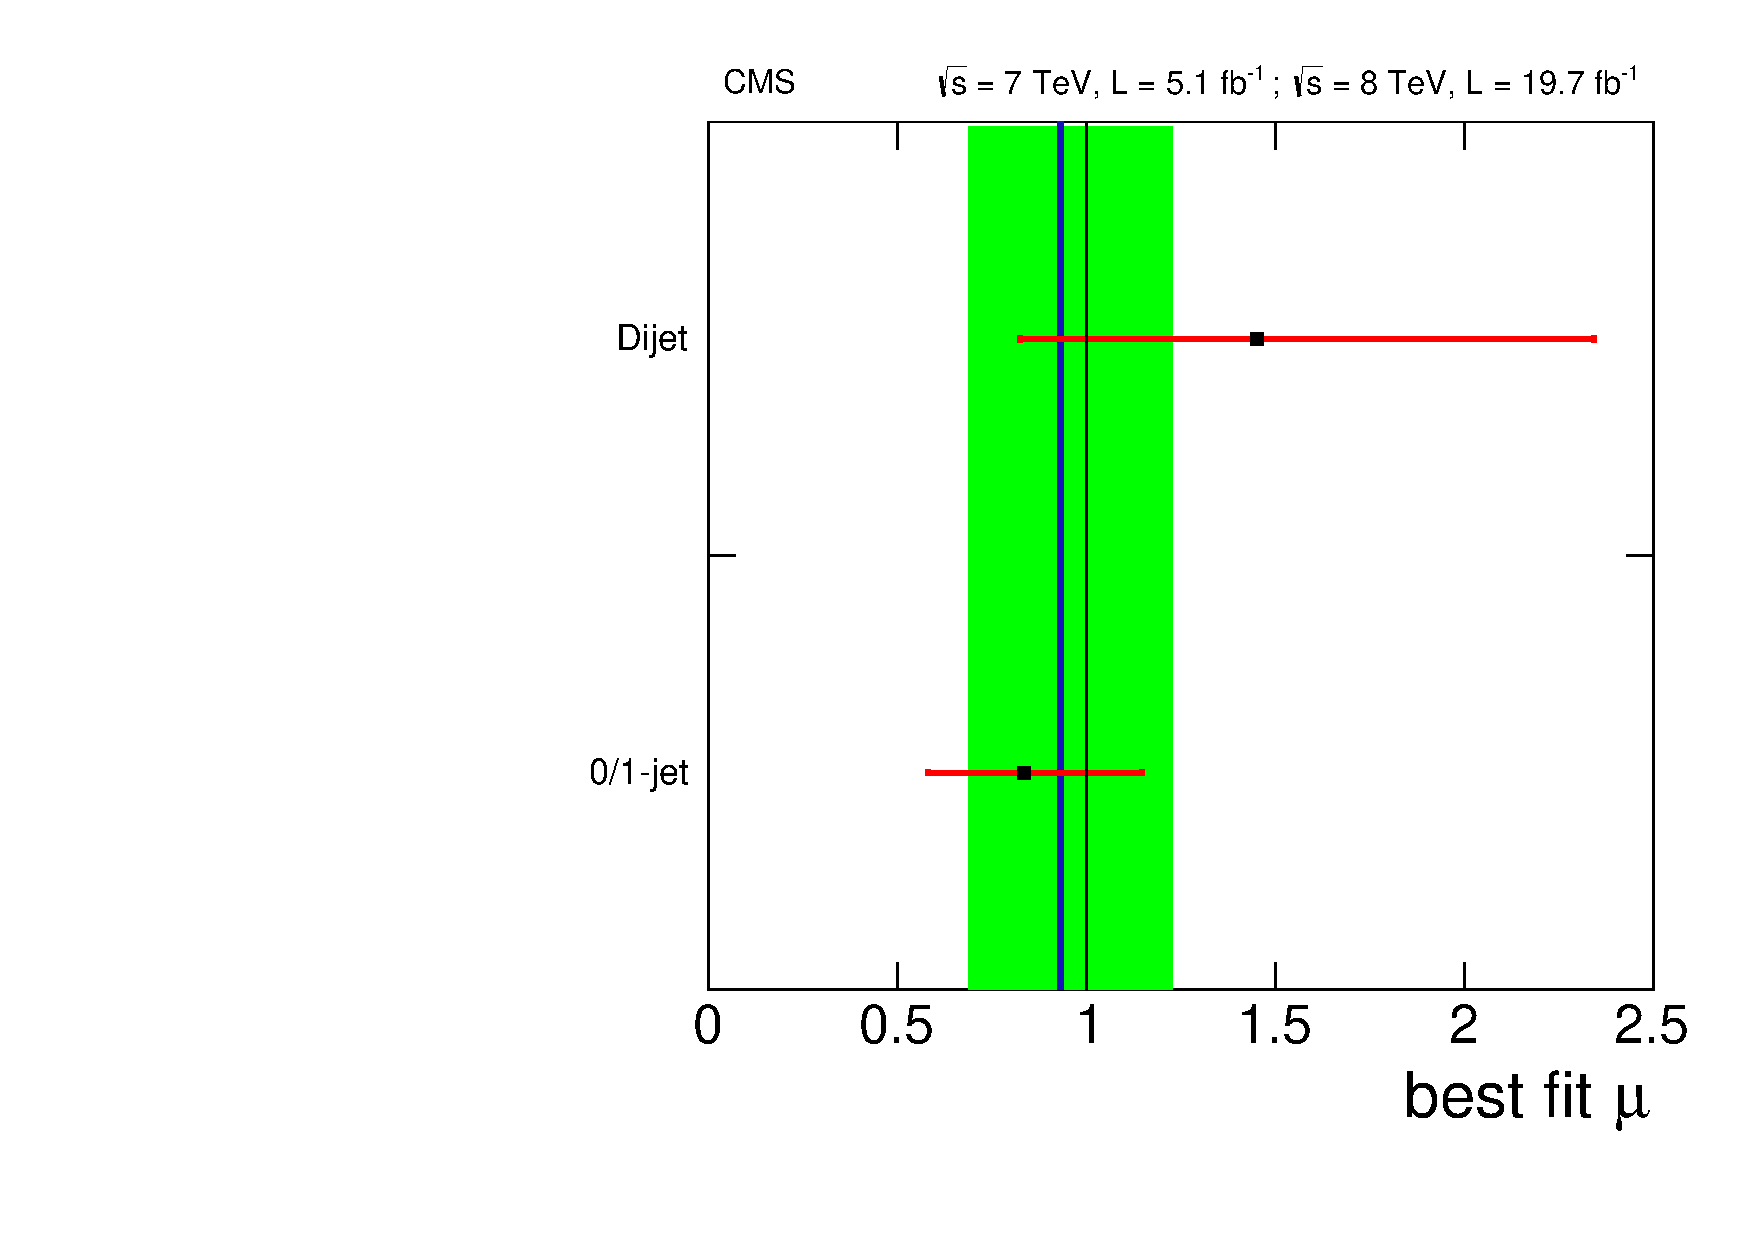
\includegraphics[width=0.45\textwidth]{HZZ4l_search/mu_bestfit_bycategory.pdf}
    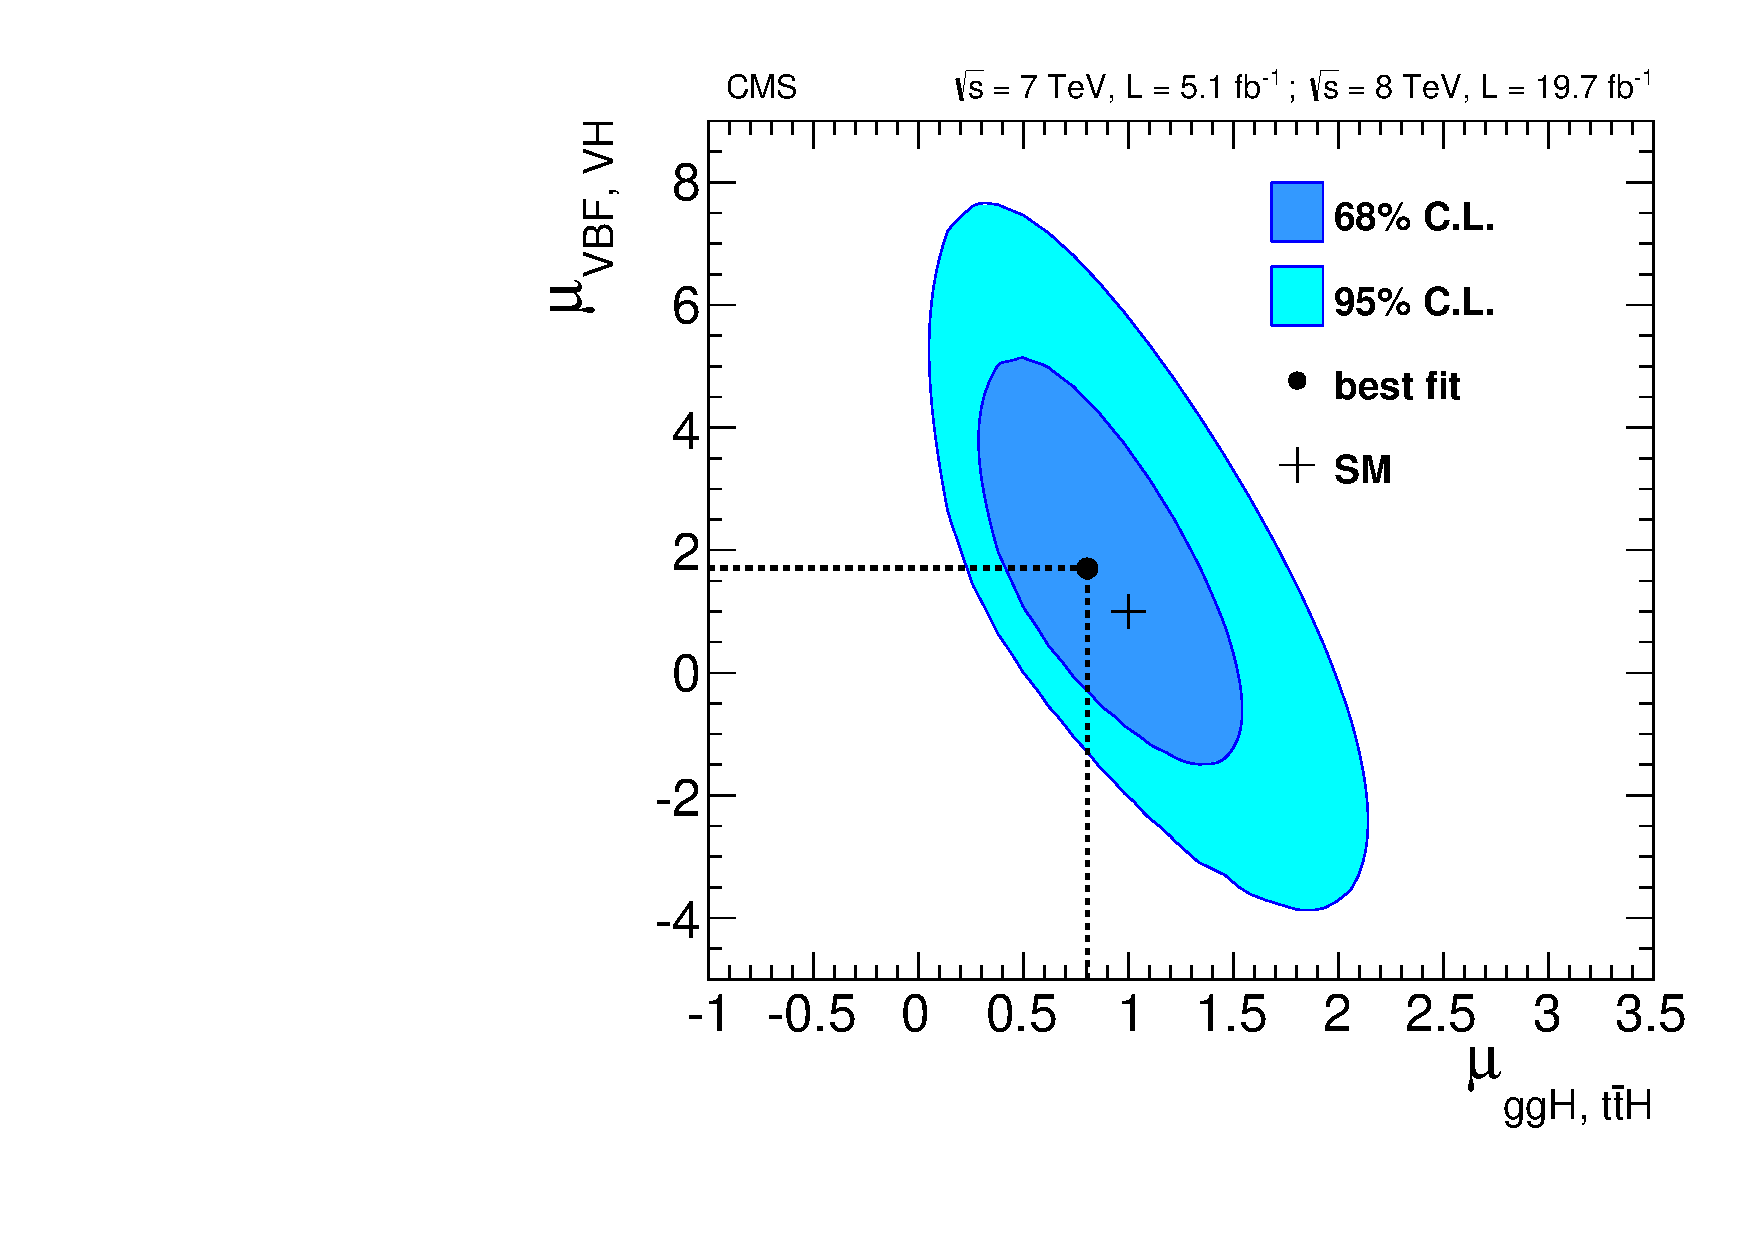
\includegraphics[width=0.45\textwidth]{HZZ4l_search/RVRF.pdf}
    \caption[(left) Values of $\mu$ for the two
    categories. The vertical line shows the combined $\mu$
    together with its associated ${\pm}1\sigma$ uncertainties, shown
    as a green band. The horizontal bars indicate the ${\pm}1\sigma$
    uncertainties in $\mu$ for the different categories. The
    uncertainties include both statistical and systematic sources of
    uncertainty.  (right) Likelihood contours on the
    signal-strength modifiers associated with fermions ($\mu_{ggH,t\bar{t}H}$) and
    vector bosons ($\mu_{\text{VBF}, VH}$) shown at a 68\% and
    95\% C.L..]{(left) Values of $\mu$ for the two
    categories. The vertical line shows the combined $\mu$
    together with its associated ${\pm}1\sigma$ uncertainties, shown
    as a green band. The horizontal bars indicate the ${\pm}1\sigma$
    uncertainties in $\mu$ for the different categories. The
    uncertainties include both statistical and systematic sources of
    uncertainty.  (right) Likelihood contours on the
    signal-strength modifiers associated with fermions ($\mu_{ggH,t\bar{t}H}$) and
    vector bosons ($\mu_{\text{VBF}, VH}$) shown at a 68\% and
    95\% C.L. \cite{Chatrchyan:2013mxa}. \label{fig:mucat}} \end{center}
\end{figure}

Two modified signal-strengths ($\mu_{ggH,t\bar{t}H}$ and $\mu_{\text{VBF}, VH}$) are introduced as scale factors for the fermion and vector-boson induced contribution to the expected SM cross section. A fit is performed for the two signal-strength modifiers simultaneously, assuming a mass hypothesis of $m_{H} = \unit{125.6}{\GeV}$. The likelihood is profiled for all nuisance parameters and 68\% and 95\% C.L. contours in the ($\mu_{ggH,t\bar{t}H}$, $\mu_{\text{VBF}, VH}$) plane are obtained. Figure~\ref{fig:mucat}~(right) shows the result of the fit leading to the measurements of $\mu_{ggH,t\bar{t}H}$ and $\mu_{\text{VBF}, VH}$. The measured values are consistent with the expectations for the SM Higgs boson, $(\mu_{ggH,t\bar{t}H}, \mu_{\text{VBF}, VH})=(1,1)$.  With the current limited statistics, we cannot establish yet the presence of VBF and $VH$ production, since $\mu_{\text{VBF}, VH}=0$ is also compatible with the data.  Since the decay (into $ZZ$) is vector-boson mediated, it is necessary that such a coupling must exist in the production side and that the SM VBF and SM $VH$ production mechanisms must be present. The fitted value of $\mu_{\text{VBF}, VH} = 1.7^{+2.2}_{-2.1}$ is driven partly by the hard $\mathcal{D}_{\text{jet}}$ spectrum of the events observed in data when compared to the expectation from the production of the SM Higgs boson (figure~\ref{fig:DpTLow}). While the fitted value of $\mu_{ggH,t\bar{t}H} = 0.80^{+0.46}_{-0.36}$ is very close to the SM expectations and dominates the measurement of the total signal strength.
